%% Definisco la classe del documento: va specificato il formato della carta,
%% le dimensioni del carattere, di cominciare i nuovi capitoli a destra e
%% fronte-retro
\documentclass[a4paper,12pt,openright,twoside,titlepage]{book}

%% Imposto l'inglese
\usepackage[italian,english]{babel}

%% Imposto l'encoding dei caratteri. Specificando utf8 posso mettere
%% direttamente le accentate senza errori
\usepackage[utf8]{inputenc}
\usepackage[T1]{fontenc}

%% Uso il template di frontespizio di Gregorio
%\usepackage{frontespizio}

\usepackage{fancyhdr}

%% Formato del titolo dei capitoli
\usepackage[Lenny]{fncychap}
\ChNumVar{\fontsize{76}{80}\usefont{OT1}{pzc}{m}{n}\selectfont}
\ChTitleVar{\centering\Large\sffamily\bfseries}

%% Font (sceglierne uno)
\usepackage{mathpazo} % Use the Palatino font by default

%% Imposto l'indentazione per ogni paragrafo
\usepackage{indentfirst}

%% Lettera iniziale del capitolo su più righe
\usepackage{lettrine}

%% Per abilitare il simbolo del trademark
\usepackage{textcomp}

%% Interlinea a 1,5
\usepackage{setspace}
\onehalfspacing % interlinea 1.5
%\singlespacing %interlinea 1
%\doublespacing % interlinea 2

%% Questo per aforismi e citazioni
\usepackage{epigraph}

%% Per inserire gli url all'interno del testo
\usepackage[hidelinks]{hyperref}
%\hypersetup{
%	colorlinks=true,
%	linkcolor=blue,
%	filecolor=magenta,      
%%	citecolor=blue
%}
%
% \urlstyle{same}

%% Per inserire codici sorgenti
\usepackage{listings}
\usepackage{verbatim}
\usepackage{xcolor}
\definecolor{mygreen}{rgb}{0,0.6,0}
\definecolor{mygray}{rgb}{0.5,0.5,0.5}
\definecolor{mymauve}{rgb}{0.58,0,0.82}
\definecolor{backcolour}{rgb}{0.95,0.95,0.92}
\definecolor{backcolourtext}{rgb}{0.85,0.85,0.82}
\lstset{ 
	postbreak=\mbox{\textcolor{red}{$\hookrightarrow$}\space},
	language=Python,
	backgroundcolor=\color{backcolour},   % choose the background color; you must add \usepackage{color} or \usepackage{xcolor}; should come as last argument
	basicstyle=\small\ttfamily,        % the size of the fonts that are used for the code
	breakatwhitespace=false,         % sets if automatic breaks should only happen at whitespace
	breaklines=true,                 % sets automatic line breaking
	captionpos=b,                    % sets the caption-position to bottom
	commentstyle=\color{mygray},    % comment style
	escapeinside={\%*}{*)},          % if you want to add LaTeX within your code
	extendedchars=true,              % lets you use non-ASCII characters; for 8-bits encodings only, does not work with UTF-8
	deletekeywords={path},
	morekeywords={def},
	frame=none,	                   % adds a frame around the code
	keepspaces=true,                 % keeps spaces in text, useful for keeping indentation of code (possibly needs columns=flexible)
	keywordstyle=\color{blue},       % keyword style
	numbers=left,                    % where to put the line-numbers; possible values are (none, left, right)
	numbersep=5pt,                   % how far the line-numbers are from the code
	numberstyle=\tiny\color{mygray}, % the style that is used for the line-numbers
	rulecolor=\color{black},         % if not set, the frame-color may be changed on line-breaks within not-black text (e.g. comments (green here))
	showspaces=false,                % show spaces everywhere adding particular underscores; it overrides 'showstringspaces'
	showstringspaces=false,          % underline spaces within strings only
	showtabs=false,                  % show tabs within strings adding particular underscores
	stepnumber=1,                    % the step between two line-numbers. If it's 1, each line will be numbered
	% stringstyle=\color{mygreen},     % string literal style
	tabsize=2,	                   % sets default tabsize to 2 spaces
	aboveskip=2.5mm,
	belowskip=2.5mm,
	xleftmargin=5mm,
	xrightmargin=5mm
}

%% Box colorati per teoremi, congetture, regole e altro.
%% Per aggiungere il bordo, usare l'opzione "frame" allo stesso
%% modo di "center", standalone
\usepackage{tcolorbox}
\usepackage{adjustbox}
\usepackage{varwidth}
\newenvironment{rulebox}{%
	\noindent
	\adjustbox{innerenv={varwidth}[l]{0.9\linewidth},margin=\fboxsep+.25cm \fboxsep+.2cm,bgcolor=backcolour,center}\bgroup
}{%
\egroup
}

%% Elenchi puntati e affini
\usepackage{enumitem}

%% Per includere le immagini e gestione lista figure e tabelle:
%% package e path dove andare a richiamarle per nome
\usepackage{graphicx}
\graphicspath{{./figures/}}
% Subfigures
\usepackage[labelfont=bf]{caption}
\usepackage{subcaption}
\captionsetup[lstlisting]{font={small,it}}
\captionsetup[figure]{font={small,it}}
\captionsetup[subfigure]{font={smaller,it}}
\captionsetup[table]{font={smaller,it}}
%\renewcommand{\listfigurename}{List of plots}
%\renewcommand{\listtablename}{Tables}

%% Questo serve per includere le immagini dove voglio io e non dove
%% pare all'editor!
\usepackage{float}

%% Fa sì che le tabelle possano essere divise tra più pagine
\usepackage{longtable}

%% Numeri di riga nelle pagine -> SOLO PER LE CORREZIONI!!
\usepackage{lineno}

%% Bibliografia
\usepackage[sorting=none,style=numeric-comp,backend=bibtex,maxbibnames=999,urldate=iso,date=iso]{biblatex}
\usepackage{csquotes}
\addbibresource{biblio/bibliography.bib} % Database con le citazioni

%% Formattazioni varie
\newcommand{\fncyblank}{\fancyhf{}}

\pagestyle{fancy}\addtolength{\headwidth}{20pt}
\renewcommand{\chaptermark}[1]{\markboth{\thechapter.\ #1}{}}
\renewcommand{\sectionmark}[1]{\markright{\thesection \ #1}{}}
\cfoot{}

%%Testatine
%\rhead[\fancyplain{}{\bfseries\leftmark}]{\fancyplain{}{\bfseries\thepage}}
%\lhead[\fancyplain{}{\bfseries\thepage}]{\fancyplain{}{\bfseries\rightmark}}

%Pagine pari
\fancyhead[RE]{\bfseries\rightmark}
\fancyhead[LE]{\bfseries\thepage}
\fancyhead[CE]{}
%\fancyfoot[LE]{\bfseries\thepage}
%\fancyfoot[CE]{}
%\fancyfoot[LE]{\textit{thesistitle}}

%Pagine dispari
\fancyhead[LO]{\bfseries\leftmark}
\fancyhead[RO]{\bfseries\thepage}
\fancyhead[CO]{}
%\fancyfoot[LO]{\bfseries\leftmark}
%\fancyfoot[CO]{}
%\fancyfoot[RO]{\textit{thesistitle}}
%\renewcommand{\footrulewidth}{0.4pt}

\fancypagestyle{plain}{%
	\fancyhf{}
	\fancyfoot[RO]{}
	\fancyfoot[LO]{}
	\fancyfoot[CO]{\bfseries\thepage}
	\renewcommand{\headrulewidth}{0pt}
	\renewcommand{\footrulewidth}{0pt}}

%% Includo subsubsection nella numerazione della TOC
\setcounter{tocdepth}{3}
\setcounter{secnumdepth}{3}

%###### Inizio documento ######%
\begin{document}

%###### Frontespizio ######%

%%
%% Titolo della tesi, relatori et similia
%%
\newcommand{\thesistitle}{Towards Process Comprehension of Industrial Control Systems: a Framework for Analyzing Industrial Systems}
\newcommand{\supervisor}{Prof. \textbf{Massimo \textsc{Merro}}}
\newcommand{\firstcosupervisor}{Prof. \textbf{Ruggero \textsc{Lanotte}}\\University of Insubria}
\newcommand{\secondcosupervisor}{\textbf{Marco \textsc{Lucchese}}}
\newcommand{\opponent}{Prof. \textbf{Mariano \textsc{Ceccato}}}
\newcommand{\candidate}{\textbf{Marco \textsc{Oliani}}\\VR457249}
\newcommand{\academicyear}{\normalsize Academic Year 2022/2023}

\begin{titlepage}
	\begin{center}
		\thispagestyle{empty}
		
		% Upper part of the page. The '~' is needed because \\
		% only works if a paragraph has started.
		
		\textsc{\Large\bfseries University of Verona}\\
		\hrulefill \\[0.1cm]
		\large Department of \textsc{COMPUTER SCIENCE}\\[1.0cm]
		
		\normalsize Master's Degree in \\
		\normalsize\textsc{COMPUTER SCIENCE AND ENGINEERING}\\[1.5cm]
		
		\large Master Thesis \\[1.0cm]
		
		% Title
		%{ \Large\bfseries\MakeUppercase{\thesistitle}}
		{ \Large\bfseries\thesistitle} \\[3.0cm]
		
		% Author and supervisor
		\begin{minipage}[t]{0.45\textwidth}
			\begin{flushleft} \normalsize
				\emph{Candidate:} \\
				\candidate
			\end{flushleft}
		\end{minipage}
		\begin{minipage}[t]{0.45\textwidth}\raggedleft
			\begin{flushright} \normalsize
				\emph{Supervisor:}\\
				\supervisor 
			\end{flushright}
			\begin{flushright} \normalsize
				\emph{Co-supervisor:}\\
				\firstcosupervisor \\
				%\secondcosupervisor
			\end{flushright}
		\end{minipage}
		
		\vfill
		
		\hrulefill \\[0.1cm]
		% Bottom of the page -> è la data
		\academicyear
		
	\end{center}
\end{titlepage}

\thispagestyle{empty}

%###### Aforisma ######%
\begin{titlepage}
	\thispagestyle{empty}
	\begin{flushright}
		\vspace*{40 mm}
		%\small{\emph{``If debugging is the process of removing software bugs,\\ then programming must be the process of putting them in.''}\\(Edsger Dijkstra)}
		
		\small{\emph{``Someone cracked my password.\\Now I need to rename my puppy.''}\\(Unknown)}
		
		%\small{\emph{``Never trust a computer you can’t throw out a window.''}\\(Steve Wozniak)}
	\end{flushright}	
	\vfill
\end{titlepage}
\thispagestyle{empty}

%###### ABSTRACT ######%
%% Abstract
%\newcommand{\fncyblank}{\fancyhf{}}
\newenvironment{abstract}%
{\cleardoublepage\fncyblank\null\vfill\begin{center}%
		\bfseries\Large\abstractname\end{center}}%
{\vfill\null}

\begin{titlepage}
	\begin{abstract}
		Bla bla bla
	\end{abstract}
	\vfill
\end{titlepage}
\thispagestyle{empty}

%###### ACKNOWLEDGEMENTS #####%
%%% Acknowledgements
%\newcommand{\fncyblank}{\fancyhf{}}
\newenvironment{acknowledgements}%
{\cleardoublepage\fncyblank\null\vfill\begin{center}%
		\bfseries\Large\ Acknowledgements\end{center}}%
{\vfill\null}

\begin{titlepage}
	\begin{acknowledgements}
		Non ringrazio nessuno!
	\end{acknowledgements}
	\vfill
\end{titlepage}
\thispagestyle{empty}

%% Faccio partire la numerazione normale DOPO l'indice: lo stesso indice 
%% verrà numerato in numeri romani
\frontmatter
\tableofcontents
\mainmatter

%%%%%%%%%%%%%%%%%%%%%%%%%%%%%%%%%
%       Inizio TESI             %
%%%%%%%%%%%%%%%%%%%%%%%%%%%%%%%%%

%###### CAPITOLO 1 ######%
\chapter{Introduction}
\label{intro}

\lettrine[lines=2]{L}{orem} ipsum dolor bla bla bla. Ma dove metto l'abstract? Prova di interlinea che direi posso anche andare bene, ma bisogna poi vedere il tutto come si incastra alla fine, in modo da ottenere un bel risultato alla vista. Sperando di non esagerare con gli abbellimenti, per evitare che qualcuno leggendo si incazzi e mi faccia riscrivere tutto, che non ne ho minimamente voglia...

Lorem Ipsum is simply dummy text of the printing and typesetting industry. Lorem Ipsum has been the industry's standard dummy text ever since the 1500s, when an unknown printer took a galley of type and scrambled it to make a type specimen book. It has survived not only five centuries, but also the leap into electronic typesetting, remaining essentially unchanged. It was popularised in the 1960s with the release of Letraset sheets containing Lorem Ipsum passages, and more recently with desktop publishing software like Aldus PageMaker including versions of Lorem Ipsum.

Why do we use it?
It is a long established fact that a reader will be distracted by the readable content of a page when looking at its layout. The point of using Lorem Ipsum is that it has a more-or-less normal distribution of letters, as opposed to using 'Content here, content here', making it look like readable English. Many desktop publishing packages and web page editors now use Lorem Ipsum as their default model text, and a search for 'lorem ipsum' will uncover many web sites still in their infancy. Various versions have evolved over the years, sometimes by accident, sometimes on purpose (injected humour and the like).


Where does it come from?
Contrary to popular belief, Lorem Ipsum is not simply random text. It has roots in a piece of classical Latin literature from 45 BC, making it over 2000 years old. Richard McClintock, a Latin professor at Hampden-Sydney College in Virginia, looked up one of the more obscure Latin words, consectetur, from a Lorem Ipsum passage, and going through the cites of the word in classical literature, discovered the undoubtable source. Lorem Ipsum comes from sections 1.10.32 and 1.10.33 of "de Finibus Bonorum et Malorum" (The Extremes of Good and Evil) by Cicero, written in 45 BC. This book is a treatise on the theory of ethics, very popular during the Renaissance. The first line of Lorem Ipsum, "Lorem ipsum dolor sit amet..", comes from a line in section 1.10.32.

The standard chunk of Lorem Ipsum used since the 1500s is reproduced below for those interested. Sections 1.10.32 and 1.10.33 from "de Finibus Bonorum et Malorum" by Cicero are also reproduced in their exact original form, accompanied by English versions from the 1914 translation by H. Rackham.

Where can I get some?
There are many variations of passages of Lorem Ipsum available, but the majority have suffered alteration in some form, by injected humour, or randomised words which don't look even slightly believable. If you are going to use a passage of Lorem Ipsum, you need to be sure there isn't anything embarrassing hidden in the middle of text. All the Lorem Ipsum generators on the Internet tend to repeat predefined chunks as necessary, making this the first true generator on the Internet. It uses a dictionary of over 200 Latin words, combined with a handful of model sentence structures, to generate Lorem Ipsum which looks reasonable. The generated Lorem Ipsum is therefore always free from repetition, injected humour, or non-characteristic words etc.

Where can I get some?
There are many variations of passages of Lorem Ipsum available, but the majority have suffered alteration in some form, by injected humour, or randomised words which don't look even slightly believable. If you are going to use a passage of Lorem Ipsum, you need to be sure there isn't anything embarrassing hidden in the middle of text. All the Lorem Ipsum generators on the Internet tend to repeat predefined chunks as necessary, making this the first true generator on the Internet. It uses a dictionary of over 200 Latin words, combined with a handful of model sentence structures, to generate Lorem Ipsum which looks reasonable. The generated Lorem Ipsum is therefore always free from repetition, injected humour, or non-characteristic words etc.

%###### CAPITOLO 2 ######%
\chapter{Background}
\label{background}

\section{What ICSs are}
\label{sec:what_ics_are}
\lettrine[lines=2]{I}{ndustrial control systems} (ICSs) are information systems used to control industrial processes such as manufacturing, product handling, production, and distribution \cite{ics_definition}.

ICSs are often found in critical infrastructure facilities such as power plants, oil and gas refineries, and chemical plants.

\bigskip
ICSs are different from traditional IT systems in several key ways. Firstly, ICSs are designed to control physical processes, whereas IT systems are designed to process and store data. This means that ICSs have different requirements for availability, reliability, and performance. Secondly, ICSs are typically deployed in environments that are harsh and have limited resources, such as extreme temperatures and limited power. Thirdly, the protocols and hardware used in ICSs are often proprietary and not widely used outside of the industrial sector.

\bigskip
ICSs are becoming increasingly connected to the internet and other networks, which has led to increased concerns about their security. Industrial systems were not originally designed with security in mind, and many of them have known vulnerabilities that could be exploited by attackers. Additionally, the use of legacy systems and equipment can make it difficult to implement security measures. As a result, ICSs are increasingly seen as a potential target for cyber attacks, which could have serious consequences for the safe and reliable operation of critical infrastructure.

\bigskip
The increasing connectivity of ICSs and the associated security risks have led to a growing interest in the field of ICS security. Researchers and practitioners are working to develop new security technologies, standards, and best practices to protect ICSs from cyber attacks. This includes efforts to improve the security of ICS networks and devices, as well as the development of new monitoring and detection techniques to identify and respond to cyber attacks.

\section{ICS components}
\label{sec:ics_components}
\textit{Industrial control systems} (ICSs) are composed of several different components that work together to monitor and control industrial processes. 

\subsection{SCADA systems}
\textit{Supervisory control and data acquisition} (\textbf{SCADA}) is a system of software and hardware elements that allows industrial organizations to \cite{scada_definition}:
\begin{itemize}
	\item Control industrial processes locally or at remote locations
	\item Monitor, gather, and process real-time data
	\item Directly interact with devices such as sensors, valves, pumps, motors, and more through human-machine interface (HMI) software
	\item Record events into a log file
\end{itemize}

The SCADA software processes, distributes, and displays the data, helping operators and other employees analyze the data and make important decisions.

\bigskip
SCADA systems are known for their ability to monitor and control large-scale industrial processes, and for their ability to operate over long distances. This makes them well-suited for use in remote locations or for controlling processes that are spread out over a wide area. However, the same features that make SCADA systems so useful also make them vulnerable to cyber attacks.

SCADA systems were not originally designed with security in mind, and many of them have known vulnerabilities that could be exploited by attackers. Additionally, the use of legacy systems and equipment can make it difficult to implement security measures. As a result, SCADA systems are increasingly seen as a potential target for cyber attacks, which could have serious consequences for the safe and reliable operation of critical infrastructure.

To secure SCADA systems, it is important to implement security measures such as network segmentation, secure communication protocols, and access control. Additionally, it is important to monitor SCADA systems for unusual activity and to implement incident response procedures to quickly detect and respond to any security breaches.

\subsubsection{Scada architecture}
\begin{figure}[ht]
	\centering
	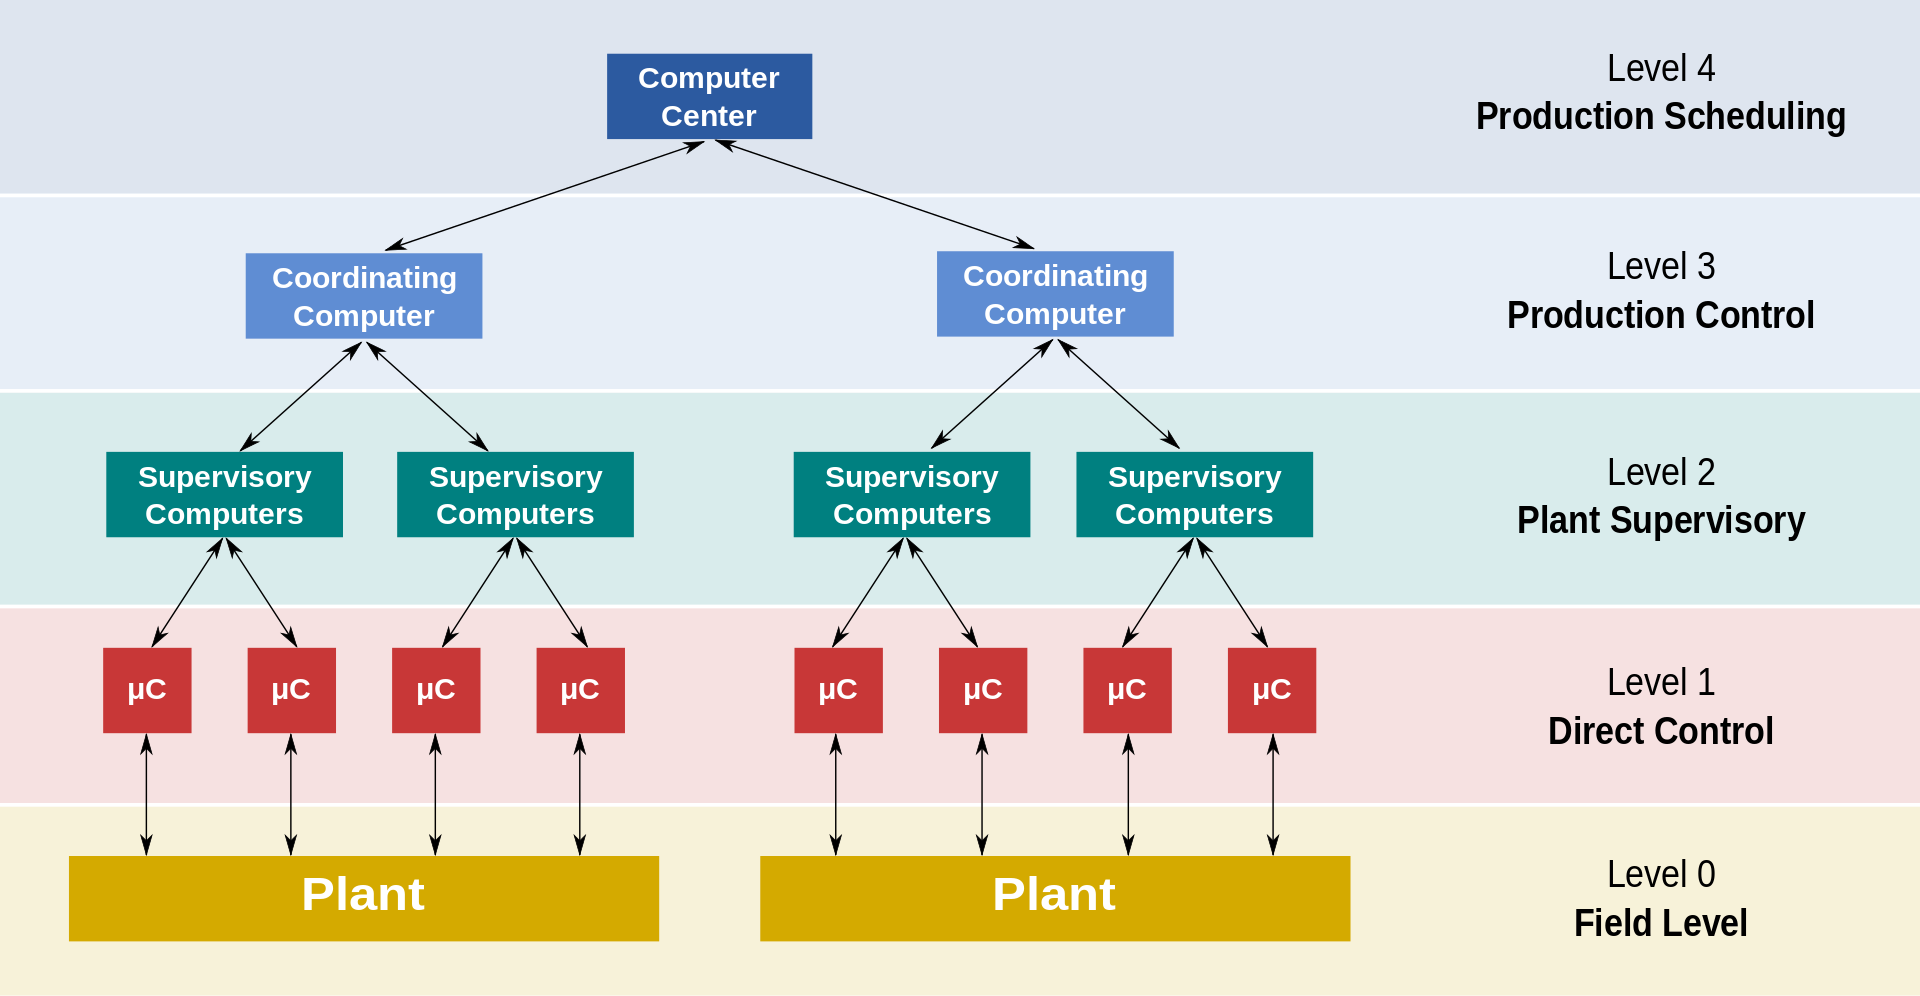
\includegraphics[scale=0.20]{layers_scada_architecture_wiki.png}
	\caption{SCADA architecture schema}
	\label{fig:SCADA_schema}
\end{figure}

SCADA architecture consists in \textbf{five layers} (Figure \ref{fig:SCADA_schema}):

\begin{itemize}
	\item Level 0 (\textbf{Field Level}): contains \textbf{field devices} (\ref{subsec:field_devs}), or \textit{sensors}.
	\item Level 1 (\textbf{Direct Control}): includes \textbf{local or remote controllers} such as \textbf{PLCs} (\ref{subsec:plc}) and \textbf{RTUs} (\ref{subsec:rtu}). Controllers interface directly to the field devices reading data from sensors and sending commands to actuators.
	\item Level 2 (\textbf{Plant Supervisory}): contains computer systems that \textbf{collate and store informations} from the previous level and provide a \textbf{Human-Machine Interface} (\textit{HMI}, \ref{subsec:hmi}) for operator control.
	\item Level 3 (\textbf{Production Control}): collect and aggregates data from the Plant Supervisory level to generate \textbf{reporting} to the Production Scheduling layer.
	\item Level 4 (\textbf{Production Scheduling}): includes business systems (such as ERP systems) used to \textbf{manage ongoing processes}.
\end{itemize}

Production Control level and Production Scheduling level are not directly connected to the process control, but concerned with monitoring production and targets and production scheduling level.

\subsection{Field devices}
\label{subsec:field_devs}
\textit{Field devices} are the \textbf{sensors} and \textbf{actuators} that are used to collect data from the process and control it. Examples of field devices include temperature sensors, pressure sensors, valves and pumps.
%
%\subsection{IED} 
%todo

\subsection{PLC}
\label{subsec:plc}
A \textit{Programmable Logic Controller} (PLC) is a \textbf{small and specialized industrial computer} having the capability of controlling complex industrial and manifacturing processes \cite{plc_definition}.

\bigskip
Compared to relay systems and personal computers, PLCs are optimized for control tasks and industrial environments: they are rugged and designed to withdraw harsh conditions such as dust, vibrations, humidity and temperature: they have more reliability than personal computers, which are more prone to crash, and they are more compact a require less maintenance than a relay system.
Furthermore, I/O interfaces are already on the controller, so PLCs are easier to expand with additional I/O modules (if in a rack format) to manage more inputs and ouputs, without reconfiguring hardware as in relay systems when a reconfiguration occours. 

\bigskip
PLCs are more \textit{user-friendly}: they are not intended (only) for computer programmers, but designed for engineers with a limited knowledge in programming languages: control program can be entered with a simple and intuitive language based on logic and switching operations instead of a general-purpose programming language (\textit{i.e.} C, C++, ...). 

\subsubsection{PLC Architecture}
The basic hardware architecture of a PLC consists of these elements \cite{plc_book}:

\begin{figure}[ht]
	\centering
	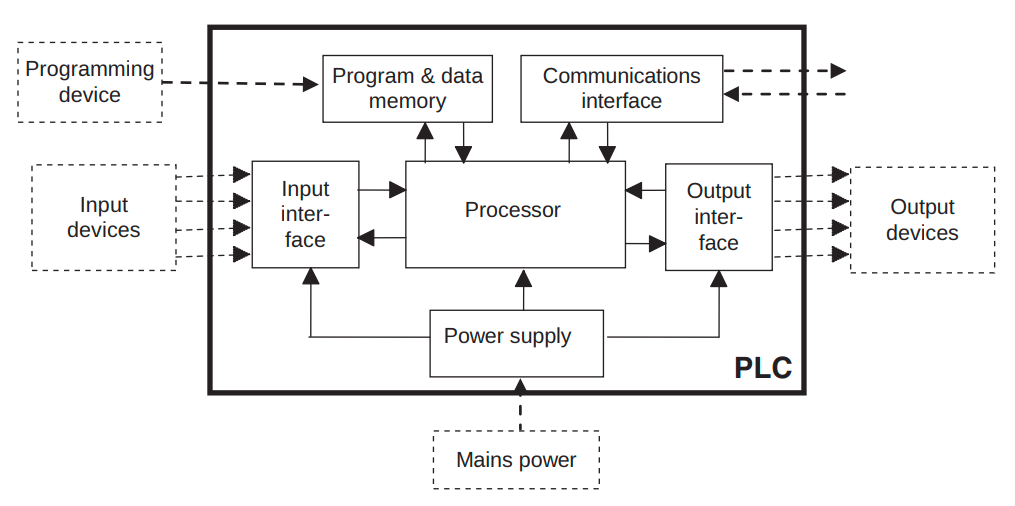
\includegraphics[scale=0.35]{plc_architecture.png}
	\caption{PLC architecture}
	\label{fig:PLC_architecture}
\end{figure}

\begin{itemize}
	\item \textbf{Processor unit (CPU)}: contains the microprocessor. This unit interpretes the input signals from I/O modules, executes the control program stored in the Memory Unit and sends the output signals to the I/O Modules.
	The processor unit also sends data to the Communication interface, for the communication with additional devices.
	\item \textbf{Power supply unit:} converts AC voltage to low DC voltage.
	\item \textbf{Programming device:} is used to store the required program into the memory unit.
	\item \textbf{Memory Unit:} consists in RAM memory and ROM memory. RAM memory is used for storing data from inputs, ROM memory for storing operating system, firmware and user program to be executed by the CPU.
	\item \textbf{I/O modules:} provide interface between sensors and final control elements (actuators).
	\item \textbf{Communications interface:} used to send and receive data on a network from/to other PLCs.
\end{itemize}

\begin{figure}[ht]
	\centering
	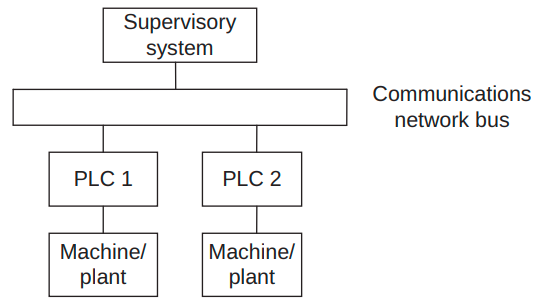
\includegraphics[scale=0.45]{plc_comm.png}
	\caption{PLC communication schema}
	\label{fig:PLC_comm}
\end{figure}

\subsubsection{PLC Programming}
\label{subsubsec:plc_programming}
Two different programs are executed in a PLC: the \textbf{operating system} and the \textbf{user program}.

\bigskip
The operating system tasks include executing the user program, managing memory areas and the \textit{process image table} (memory registers where inputs from sensors and outputs for actuators are stored).

\bigskip
The user program needs to be uploaded on the PLC via the programming device and runs on the process image table in \textit{scan cycles}: each scan is made up of three phases \cite{ceccato}:

\begin{enumerate}
	\item reading inputs from the process images table
	\item execution of the control code and computing the physical process evolution
	\item writing output to the process image table to have an effect on the physical process. At the end of the cycle, the process image table is refreshed by the CPU
\end{enumerate}

Standard PLCs \textbf{programming languages} are basically of two types: \textbf{textuals} and \textbf{graphicals}.
Textual languages include languages such as \textit{Instruction List} (IL) and \textit{Structured Text} (ST), while \textit{Ladder Diagrams} (LD), \textit{Function Block Diagram} (FBD) and \textit{Sequential Function Chart} (SFC) belong to the graphical languages.

\bigskip
Graphical languages are more simple and immediate comparing to the textual ones and are preferred by programmers because of their features and simplicity, in particular the \textbf{Ladder Logic programming} (see Figure \ref{fig:st_ll_comparison} for a comparison).

\begin{figure}[ht]
	\centering
	\begin{subfigure}{0.47\textwidth}
		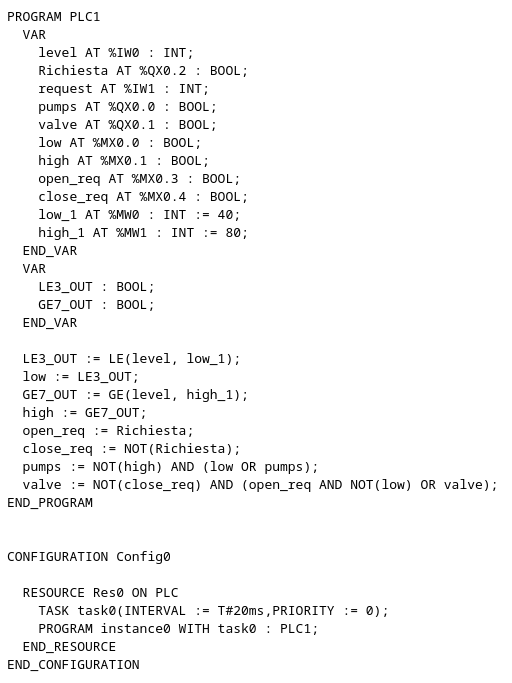
\includegraphics[scale=0.30]{st.png}
		\caption{Example of ST programming}
		\label{subfig:st_example}
	\end{subfigure}
	\hfill
	\begin{subfigure}{0.47\textwidth}
		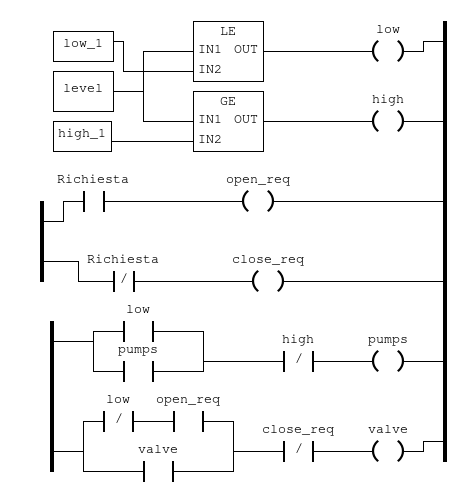
\includegraphics[scale=0.55]{ll.png}
		\caption{Example of Ladder Logic}
		\label{subfig:ladder_logic_example}
	\end{subfigure}
	\caption{Comparison between ST language and Ladder Logic}
	\label{fig:st_ll_comparison}
	
\end{figure}

\subsubsection{PLC Security}
\label{subsubsec:plc_security}
PLCs were originally designed to operate as closed systems, not connected and exposed to the outside world via communication networks: the question of the safety of these systems, therefore, was not a primary aspect. The advent of  Internet has brought undoubted advantages, but has introduced problems relating to the safety and protection of PLCs from external attacks and vulnerabilities.

Indeed, a variety of different communication protocols used in ICSs are designed to be efficient in communications, but do not provide any security measure i.e. confidentiality, authentication and data integrity, which makes these protocols vulnerable against many of the IT classic attacks such as \textit{Replay Attack} or \textit{Man in the Middle Attack}. 

\bigskip
Countermeasures to enhance security in PLC systems may include \cite{plc_security}:
\begin{itemize}
	\item protocol modifications implementing \textbf{data integrity}, \textbf{authentication} and \textbf{protection} against \textit{Replay Attacks}
	\item use of \textit{Intrusion Detection and Prevention Systems} (IDP) 
	\item creation of \textit{Demilitarized Zones} (DMZ) on the network
\end{itemize}

In addition to this, keeping the process network and Internet separated, limiting the use of USB devices among users to reduce the risks of infections, and using strong account management and maintenance policies are best practices to prevent attacks and threats and to avoid potential damages. 

\subsection{RTU}
\label{subsec:rtu}
\textit{Remote Terminal Units} (RTUs) are computers with radio interfacing similar to PLCs: they transmit telemetry data to the control center or to the PLCs and use messages from the master supervisory system to control connected objects \cite{rtu_definition}.

\bigskip
The purpose of RTUs is to operate efficiently in remote and isolated locations by utilizing wireless connections. In contrast, PLCs are designed for local use and rely on high-speed wired connections. This key difference allows RTUs to conserve energy by operating in low-power mode for extended periods using batteries or solar panels. As a result, RTUs consume less energy than PLCs, making them a more sustainable and cost-effective option for remote operations.

\bigskip
Industries that require RTUs often operate in areas without reliable access to the power grid or require monitoring and control substations in remote locations. These include telecommunications, railways, and utilities that manage critical infrastructure such as power grids, pipelines, and water treatment facilities. The advanced technology of RTUs allows these industries to maintain essential services, even in challenging environments or under adverse weather conditions.

\subsection{HMI}
\label{subsec:hmi}
The \textit{Human-Machine Interface} (HMI) is the hardware and software interface that operators use to monitor the processes and interact with the ICS. 

An HMI shows the operator and authorized users information about system status and history; it also allows them to configure parameters on the ICS such as set points and, send commands and make control decisions \cite{hmi_definition}.

The HMI can be in the form of a physical panel, with buttons and indicator lights, or PC software.

\subsection{Cybersecurity components}
\textit{Cybersecurity components}, as seen in section \ref{subsubsec:plc_security} about PLCs security, are used to protect  ICSs from cyber threats and vulnerabilities. They can include firewalls, \textit{Intrusion Detection and Prevention systems} (IDP), and \textit{Security Information and Event Management} (SIEM) systems.

\subsection{Communication Networks}
\textit{Communication Networks} are the networks that are used to connect the different components of the ICS and allow them to communicate with each other. Communication networks can include wired and wireless networks, such as Ethernet/IP, Modbus, and DNP3 (see Section \ref{sec:ics_protocols}).

\section{ICS Communication Protocols}
\label{sec:ics_protocols}
As mentioned in Section \ref{sec:what_ics_are}, industrial systems differ from classical IT systems in the purpose for which they are designed: controlling physical processes the former, processing and storing data the latter. For this reason, ICSs require different communication protocols than traditional IT systems for real time communications and data transfer.

\bigskip
A wide variety of industrial protocols exists: this is because originally each vendor developed and used its own proprietary protocol. However, these protocols were often incompatible with each other, resulting in devices from different vendors being unable to communicate with each other.

To solve this problem, standards were defined with a view to allowing these otherwise incompatible device to intercommunicates.

\bigskip
Among all the various protocols, some have risen to prominence as widely accepted standards. These \textit{de facto} protocols are commonly utilized in industrial systems due to their proven reliability and effectiveness. In the following sections, we will provide a brief overview of some of the most prevalent and widely used protocols in the industry.

\subsection{Modbus}
\label{subsec:modbus}
\textit{Modbus} is a serial communication protocol developed by Modicon (now Schneider Electric) in 1979 for use with its PLCs \cite{Modbus_definition} and designed expressly for industrial use: it facilitates interoperability of different devices connected to the same network (sensors, PLCs, HMIs, ...) and it is also often used to connect RTUs to SCADA acquisition systems.

\bigskip
Modbus is the most widely used communication protocol among industrial systems because it has several advantages:

\begin{itemize}
	\item simplicity of implementation and debugging
	\item it moves raw bits and words, letting the individual vendor to represent the data as it prefers
	\item it is, nowadays, an \textbf{open} and \textbf{\textit{royalty-free}} protocol: there is no need to sustain licensing costs for implementation and use by industrial device vendors
\end{itemize}

Modbus is a \textbf{request/response} (or \textit{master/slave}) protocol: this makes it independent of the transport layer used.

\begin{figure}[ht]
	\centering
	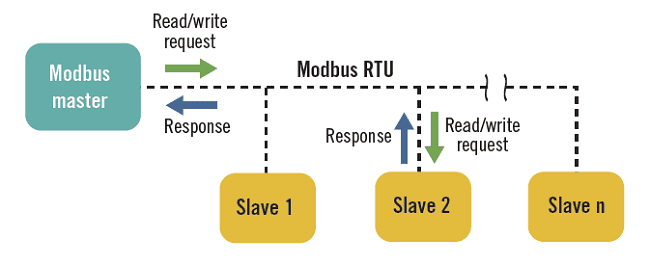
\includegraphics[scale=0.50]{Modbus_RequestResponse.png}
	\caption{Modbus Request/Response schema}
	\label{fig:modbus_requestresponse}
\end{figure}

In this kind of architecture, a single device (master) can send requests to other devices (slaves), either individually or in broadcast: these slave devices (usually peripherals such as actuators) will respond to the master by providing data or performing the action requested by the master using the Modbus protocol. Slave devices cannot generate requests to the master \cite{Modbus_rr}.

\bigskip
There are several variants of Modbus, of which the most popular and widely used are Modbus RTU (used in serial port connections) and Modbus TCP (which instead uses TCP/IP as the transport layer).
Modbus TCP embeds a standard Modbus frame in a TCP frame (see Figure \ref{fig:modbus_frames}): both masters and slaves listen and receive data via TCP port 502.

\begin{figure}[ht]
	\centering
	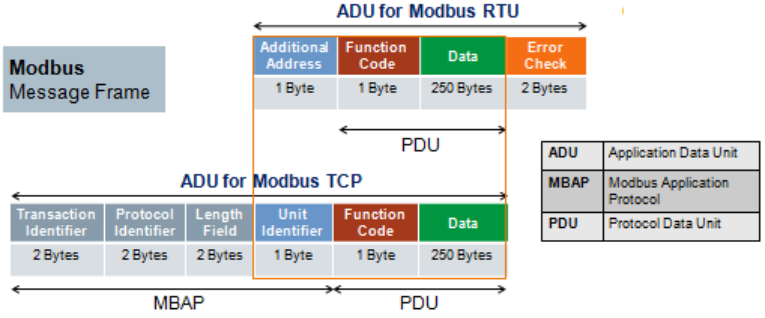
\includegraphics[scale=0.50]{modbus_frames.png}
	\caption{Modbus RTU frame and Modbus TCP frame}
	\label{fig:modbus_frames}
\end{figure}

\subsubsection{Modbus registers}
\label{subsub:modbus_registers}
Modbus provides four object types, which map the data accessed by master and slave to the PLC memory:

\begin{itemize}
	\item \textit{Coil}: binary type, read/write accessible by both masters and slaves
	\item \textit{Discrete Input}: binary type, accessible in read-only mode by masters and in read/write mode by slaves
	\item \textit{Analog Input}: 16 bits in size (word), are accessible in read-only mode by masters and in read/write mode by slaves
	\item \textit{Holding Register}:  16 bits in size (word), accessible in read/write mode by both masters and slaves. Holding Registers are the most commonly used registers for output and as general memory registers.
\end{itemize}

\subsubsection{Modbus Function Codes}
\label{subsub:modbus_func_codes}
\textit{Modbus Function Codes} are specific codes used by the Modbus master within a request frame (see Figure \ref{fig:modbus_frames}) to tell the Modbus slave device which register type to access and which action to perform on it.

\bigskip
Two types of Function Codes exists: for data access and for diagnostic
Function Codes list for data access are listed in Table \ref{table:modbus_fc_list}:

\bigskip
\begin{longtable}[c]{| c | c |}
	\hline
	\textbf{Function Code} & \textbf{Description} \\ [0.5ex] 
	\hline
	FC01 & Read Coils \\
	\hline 
	FC02 & Read Discrete Input \\
	\hline
	FC03 & Read Holding Registers \\
	\hline
	FC04 & Read Analog Input Registers \\
	\hline
	FC05 & Write/Force Single Coil \\ 
	\hline
	FC06 & Write/Force Single Holding Register \\ 
	\hline 
	FC15 & Write/Force Multiple Coils \\ 
	\hline
	FC16 & Write/Force Multiple Holding Registers \\ 
	\hline
	
	\caption{Modbus Function Codes list}
	\label{table:modbus_fc_list}
\end{longtable}

\subsubsection{Modbus Security}
\label{subsub:modbus_sec}
Despite its simplicity and widespread use, the Modbus protocol does not have any security features, which exposes it to vulnerabilities and attacks.

Data in Modbus are transmitted unencrypted (\textit{lack of confidentiality}), with no data integrity controls (\textit{lack of integrity}) and authentication checks (\textit{lack of authentication}), in addition to the \textit{lack of session}. Hence, the protocol is vulnerable to a variety of attacks, such as Denial of Services (DoS), buffer overflows and reconnaissance activities.

\bigskip
The easiest attack to bring to the Modbus protocol, however, is \textbf{packet sniffing}: since, as mentioned earlier, network traffic is unencrypted and the data transmitted is in cleartext, it is sufficient to use a packet sniffer to capture the network traffic, read the packets and thus gather informations about the system such as ip addresses, function codes of requests and to modify the operation of the devices.

\begin{figure}[ht]
	\centering
	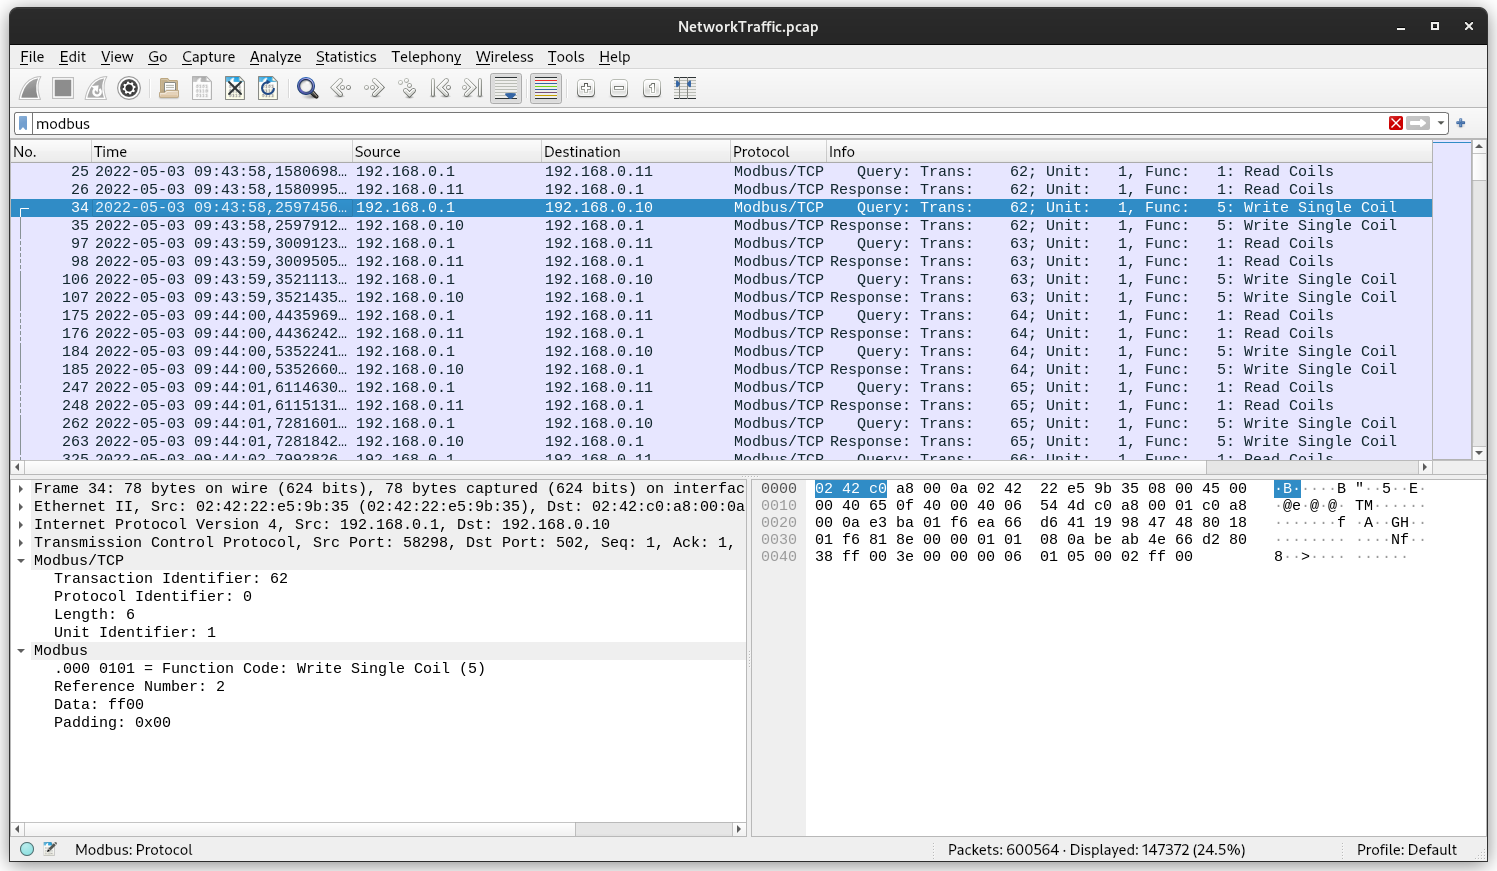
\includegraphics[scale=0.25]{modbus_packet_sniffing.png}
	\caption{Example of packet sniffing on the Modbus protocol}
	\label{fig:modbus_packet_sniffing}
\end{figure}

To make the Modbus protocol more secure, an encapsulated version was developed within the \textit{Transport Security Layer} (TLS) cryptographic protocol, also using mutual authentication. This version of the Modbus protocol is called \textbf{Secure Modbus} or \textbf{Modbus TLS}. In addition to this, Secure Modbus also includes X.509-type certificates to define permissions and authorisations \cite{modbus_tls_pdf}.

\vfill

\subsection{Ethernet/IP}
\label{sub:enip}

\subsection{Common Industrial Protocol (CIP)}
\label{sub:cip}

\subsection{Other Protocols}

\vfill



%###### CAPITOLO 3 ######%
\chapter{State of the Art}
\label{state_of_art}
\linenumbers

\lettrine[lines=2]{I}{n traditional IT}, an attacker aims to understand the behavior of a program through various techniques so as to bring attacks aimed at changing its execution flow, functionalities or bypassing limits imposed by the licensing of such software. These attack techniques include a \textbf{preliminary study} of the program: a \textit{static analysis} (i.e., a preliminary analysis of the software without it running) and a \textit{dynamic analysis} (i.e., an analysis performed with the program running).\\
The result of these two preliminary investigation techniques is a \textbf{reverse engineering} of the software, which is useful for identifying any weaknesses or bugs and therefore planning an attack.

\bigskip
In the OT context, however, the concept of \textit{reverse engineering} is also associated with that of \textit{\textbf{process comprehension}}, a term coined by Green et al.'s \cite{green_et_al} to describe the understanding of the characteristics of the system and the physical elements of within it, that are responsible for its proper functioning.

\bigskip
Not much knowledge exists in the literature regarding the collection and analysis of information concerning the understanding and operation of an ICS: in Section \ref{sec:related_work} we will look at a quick overview of some of the existing literature on the subject and in the following sections we will focus in particular on one of the papers exposed.

\vfill

\section{Literature on Process Comprehension}
\label{sec:related_work}
\begin{description}
	\item[\textit{Keliris and Maniatikos}] The first approach presented in this section is by Keliris and Maniatakos \cite{keliris_maniatakos}: they present a methodology for automating the reverse engineering of ICS binaries based on a \textit{modular framework} (called ICSREF) that can reverse binaries compiled with CODESYS, one of the most popular and widely used PLC compilers, irrespective of the language used.
	
	\item[\textit{Yuan et al.}] Yuan et al. \cite{yuan_et_al} propose a \textit{data-driven} approach to discovering cyber-physical systems from data directly: to achieve this goal, they have implemented a framework whose purpose is to identify physical systems and transition logic inference, and to seek to understand the mechanisms underlying these cyber-physical systems, making furthermore predictions concerning their state trajectories based on the discovered models.
	
	\item[\textit{Feng et al.}] Feng et al. \cite{feng_swat} developed a framework that can generate system \textit{invariant rules} based on machine learning and data mining techniques from ICS operational data log. These invariants are then selected by systems engineers to derive IDS systems from them.
	
	The experiment results on two different testbeds, the \textit{Water Distribution system} (WaDi) and the \textit{Secure Water Treatment system} (SWaT), both located at the iTrust - Center for Research in Cyber Security at the University of Singapore \cite{itrust_site}, show that under the same false positive rate invariant-based IDSs have a higher efficiency in detecting anomalies than IDS systems based on a residual error-based model. 
	
	\item[\textit{Pal et al.}] Pal et al. \cite{pal_et_al} work is somewhat related to Feng et al.'s: this paper describes a data-driven approach to identifying invariants automatically using \textit{association rules mining} \cite{association_rules_mining} with the aim of generate invariants sometimes hidden from the design layout. The study has the same objective of Feng et al.'s and uses too the iTrust SwaT System as testbed.
	
	Currently this technique is limited to only pair wise sensors and actuators: for more accurate invariants generation, the technique adopted must be capable of deriving valid constrains across multiple sensors and actuators.
	
	\item[\textit{Winnicki et al.}] Winnicki et al. \cite{winnicki_et_al} instead propose a different approach to process comprehension based on the \textbf{attacker's perspective} and not limited to mere \textit{Denial of Service} (DoS): their approach is to discover the dynamic behavior of the system, in a semi-automated and process-aware way, through \textit{probing}, that is, slightly perturbing the cyber physical system and observing how it reacts to changes and how it returns to its original state. The difficulty and challenge for the attacker is to perturb the system in such a way as to achieve an observable change, but at the same time avoid this change being seen as a system anomaly by the IDSs.
	
	\item[\textit{Green et al.}] Green et al. \cite{green_et_al} also adopt an approach based on the attacker's perspective: this approach consists of two practical examples in a \textit{Man in the Middle} (MitM) scenario to obtain, correlate, and understand all the types of information an attacker might need to plan an attack to alter the process while avoiding detection.
	
	The paper shows \textit{step-by-step} how to perform a ICS \textbf{reconnaissance}, which is fundamental to process comprenension and thus to the execution of MiTM attacks.
	
	\item[\textit{Ceccato et al.}] Ceccato et al. \cite{ceccato} propose a methodology based on a \textit{black box dynamic analysis} of an ICS using a reverse engineering tool to derive from the scans performed on the memory registers of the exposed PLCs and network scans an approximate model of the physical process. This model is obtained by inferring statistical properties, business process and system invariants from data logs.
	
	The proposed methodology was tested on a non-trivial case study, using a testbed inspired by an industrial water treatment plant.
	
	In the next section I will examine this latest work in more detail, which will be the basis for my work and thus the subsequent chapters of this thesis.

\end{description}

\section{Ceccato et al.’s methodology for analyzing water-tank systems}
\label{sec:ceccato_metodology}
As mentioned earlier, the paper proposes a methodology based on a black box dynamic analysis of an ICS by identifying potential PLCs on the network and scanning the memory registers of the identified controllers to obtain an approximate model of the controlled physical process.

\bigskip
The first objective of this black box analysis is to associate the various memory registers of the target PLCs with a correspondence to the basic concepts of an ICS such as sensors (otherwise known as measurements), actuators, setpoints (range of values of a physical variable), network communications, and so on.\\
This is performed by analyzing the different types of memory registers associated with the Modbus protocol and trying to figure out what type of data they may contain.

The second objective is to put in relation the runtime evolution of these basic concepts.

\bigskip
To achieve this, Ceccato et al. developed a prototype tool \cite{plc_re} that performs reverse engineering of the physical system through four phases:

\begin{enumerate}
	\item \textbf{scanning of the system and data pre-processing}: data gathering is performed to generate the data logs of PLCs registers
	
	\item \textbf{graphs and statistical analysis}: provides information about the memory registers using graphs and statistical data derived from the gathered data
	
	\item \textbf{invariants inference and analysis}: generates system invariants and allows user to view invariants related to a given sensor or actuator
	
	\item \textbf{business process mining and analysis}: reconstructs, from event logs, the business process that shows how process is carried out
\end{enumerate}

In Figure \ref{fig:ceccato_overview} we have a schematic representation of the workflow related to this work. We will cover all these phases in detail in the next sections of this chapter. 

\begin{figure}[ht]
	\centering
	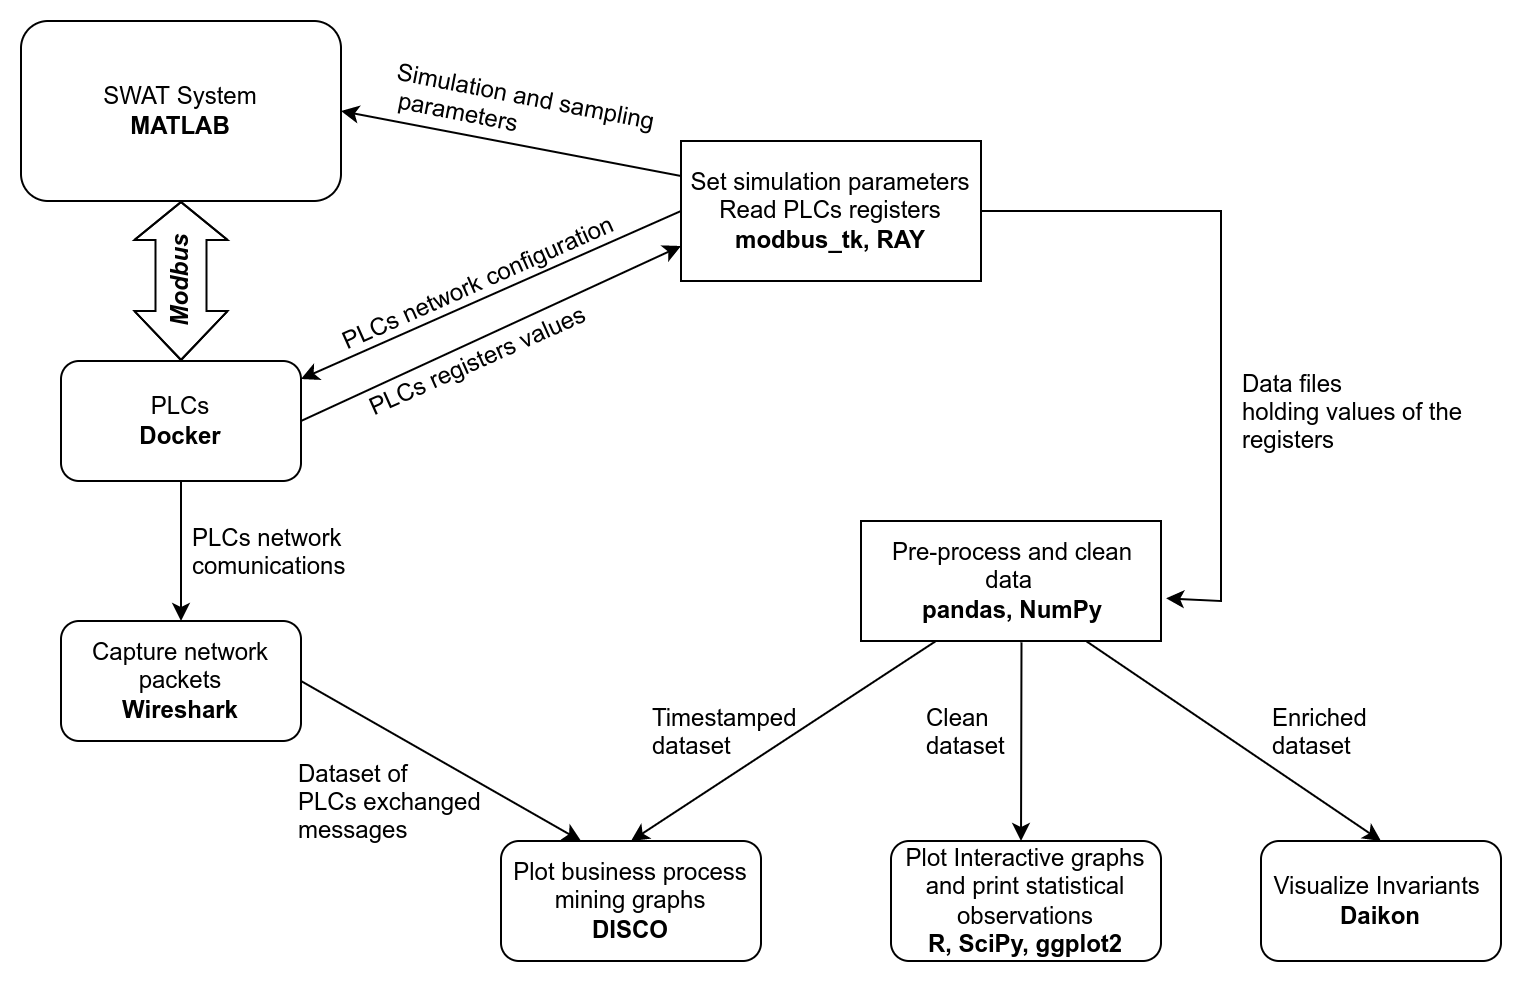
\includegraphics[scale=0.23]{chap3/ceccato_flowchart.png}
	\caption{Overview}
	\label{fig:ceccato_overview}
\end{figure}

\subsection{Testbed}
\label{subsec:ceccato_testbed}
Before describing the various phases of the methodology, let's take a look at the testbed on which this methodology will be tested. The testbed used to test this methodology is a (very) simplified version of the iTrust SWaT system \cite{swat_home} implemented by Lanotte et al. \cite{lanotte_et_al}: in Figure 3.2 we can see a graphical representation of the testbed. This simplified version consists of three stages, each controlled by a dedicated PLC: 

\begin{figure}[ht]
	\centering
	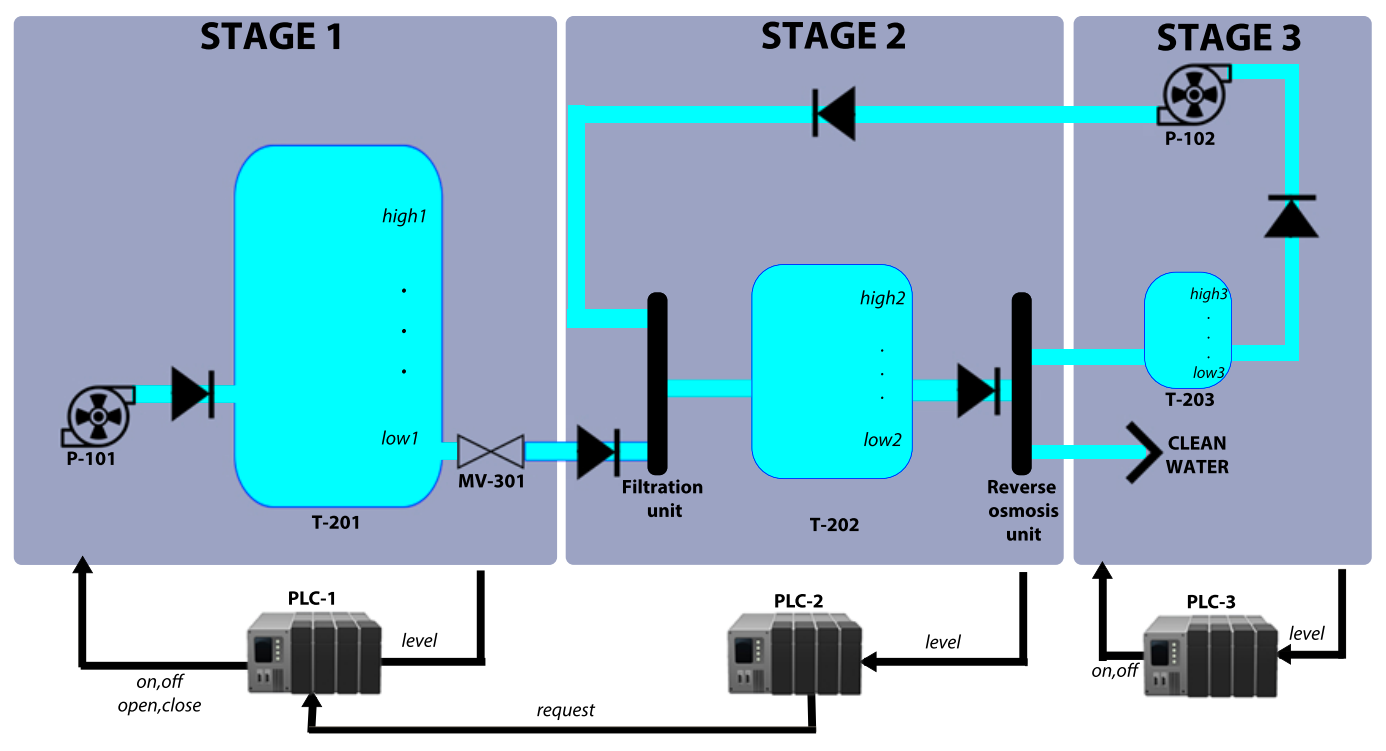
\includegraphics[scale=0.27]{chap3/univr_testbed.png}
	\caption{The simplified SWaT system used for running Ceccato et al. methodology}
	\label{fig:univr_testbed}
\end{figure}

\bigskip
\begin{description}
	\item[\textit{Stage 1}] At the first stage, a \textbf{tank} with a capacity of 80 gallons (identified by the code T-201) is filled with raw water by the P-101 pump: the MV-301 valve (where MV stands for \textit{motorized valve}), also connected to the T-201 tank, flushes out the water collected in the tank to send it to the second stage, first to the \textit{filtration unit} (here not identified by any sensor) and from there to a \textbf{second tank}, identified by the code T-202 and with a capacity of 20 gallons.
	
	\item[\textit{Stage 2}] At the second stage, water contained in T-202 flows into the \textit{reverse osmosit unit} (RO, which in this case also acts as a valve, extracting water continuously: however, it is not identified as a pump) to reduce organic impurities in the same water. The water then flows from the \textit{RO unit} to the third and last stage.
	
	\item[\textit{Stage 3}] At the third stage, the water from the \textit{RO unit} is divided according to whether standards are met: if the water is clean it will be fed into the distribution system, otherwise it will go to a \textit{backwash tank}, identified by code T-203 and a capacity of one gallon. The water in this tank will then be pumped back to the stage 2 \textit{filtration unit} through pump P-102.
\end{description}

\bigskip
As mentioned, each stage corresponds to a PLC that controls it, PLC1, PLC2 and PLC3, respectively. Let us briefly see the behavior of each of them:

\begin{description}
	\item[\textit{PLC1}] PLC1 checks the level of tank T-201 distinguishing three cases:
	
	\begin{itemize}
		\item if T-201 reaches the \textit{low setpoint low1} (hardcoded in memory registers), pump \textbf{P-101 is opened} and valve \textbf{MV-301 is closed}, so that the tank can be filled
		
		\item if T-201 reaches \textit{high setpoint high1} (also hardcoded in the memory registers), pump \textbf{P-101 is closed}
		
		\item in intermediate cases, \textbf{PLC1 waits for request from PLC2} to open/close valve MV-301: if a request to open the valve MV-301 arrives, water will flow from T-201 to T-202, otherwise the valve is closed. In both situations, pump P-101 remains closed 
	\end{itemize}

	\item[\textit{PLC2}] PLC2 monitors the level of tank T-202, behaving accordingly depending on the level of water in it. Here again there are three cases to consider:
	
	\begin{itemize}
		\item if the water level reaches the \textit{low setpoint low2} (also hardcoded in the memory registers), PLC2 sends a request to PLC1 via a Modbus channel to \textbf{open valve MV-301} in order to flow water from tank T-201 to tank T-202. The transmission channel is implemented by copying a boolean value from a memory register of PLC2 to a corresponding register of PLC1
		
		\item if the water level reaches the \textit{high setpoint high2} instead (hardcoded in the memory registers as the previous setpoints), PLC2 sends PLC1 a \textbf{close request} for valve MV-301
		
		\item In intermediate cases, the valve remains open (closed) while the tank is filling (emptying)
	\end{itemize}
	
	\item[\textit{PLC3}] PLC3 monitors the level of the T-203 backwash tank, behaving accordingly. Here there are only two cases to consider: if the tank reaches the \textit{low setpoint low3}, pump \textbf{P103 is set to off}, so that the backwash tank can be filled: otherwise, if the \textit{high setpoint high3} is reached, pump \textbf{P103 is opened} and the entire content of the backwash tank pumped back to the filter unit of T-202.
	 
\end{description} 

\subsection{Scanning of the System and Data Pre-processing}
\label{subsec:ceccato_scan}
\paragraph{Scanning tool}
The Ceccato et al. scanning tool is closely derived from a project I did \cite{ns_proj} for the "\textit{Network Security}" and "\textit{Cyber Security for IoT}" courses taught by Professors Massimo Merro and Mariano Ceccato, respectively, in the 2020/21 academic year. The original project involved, in its first part, the recognition within a network of potential PLCs listening on the standard Modbus TCP port 502 using the Nmap module for Python, obtaining the corresponding IP addresses: then a (sequential) scan of a given range of the memory registers of the found PLCs was performed to collect the register data. The data thus collected were saved to a file in \textit{JavaScript Object Notation} (JSON) format for later use in the second part of my project.

\bigskip
The scanning tool by Ceccato et. al works in a similar way, but extends what I originally did by trying to discover other ports on which the Modbus protocol might be listening (since in many realities Modbus runs on different ports than the standard one, according to the concept of \textit{security by obscurity}) and, most importantly, by \textbf{parallelizing and distributing the scan} of PLC memory registers through the Ray module \cite{ray}, specifying moreover the desired granularity of the capture. An example of raw data capture can be seen at Listing \ref{lst:raw_registers_capture}:

\begin{lstlisting}[language=Python, numbers=none, caption=Example of registers capture, label=lst:raw_registers_capture]	
	"127.0.0.1/8502/2022-05-03 12_10_00.591": {
		"DiscreteInputRegisters": {"%IX0.0": "0"},
		"InputRegisters": {"%IW0": "53"},
		"HoldingOutputRegisters": {"%QW0": "0"},
		"MemoryRegisters": {"%MW0": "40","%MW1": "80"},
		"Coils": {"%QX0.0": "0"}}
\end{lstlisting}

The captured data includes PLC's IP address, Modbus port and timestamp (first line), type and name of registers with their values read from the scan (subsequent lines).

\bigskip
The tool furthermore offers the possibility, in parallel to the memory registers scan, of \textbf{sniffing network traffic} related to the Modbus protocol using the \textit{Man in the Middle} (MitM) technique on the supervisory control network using a Python wrapper for tshark/Wireshark \cite{tshark} \cite{wireshark}. An example of raw data obtained with this sniffing can be seen in Listing \ref{lst:raw_network_capture}:

\begin{lstlisting}[language=Python, numbers=none, caption=Example of raw network capture, label=lst:raw_network_capture]	
	Time,Source,Destination,Protocol,Length,Function Code,Destination Port,Source Port,Data,Frame length on the wire,Bit Value,Request Frame,Reference Number,Info
	2022-05-03 11:43:58.158,IP_PLC1,IP_PLC2,Modbus/TCP,76,Read Coils,46106,502,,76,TRUE,25,,"Response: Trans: 62; Unit: 1, Func: 1: Read Coils"
\end{lstlisting}

\paragraph{Data Pre-processing} 
The data collected by scanning the memory registers of the PLCs are then reprocessed by a Python script and converted in order to create a distinct raw dataset in \textit{Comma Separated Value} format (CSV) for each PLC, containing the memory register values associated with the corresponding controller registers. These datasets are reprocessed again through the Python modules for \textbf{pandas} \cite{pandas} and \textbf{NumPy} \cite{numpy} by another script to first perform a \textbf{data cleanup}, removing all those memory registers that do not take values and are therefore useless within the system, \textbf{merged} into a single dataset, and finally \textbf{enriched} with additional data\footnote{Not all additional data are calculated and entered automatically by the tool: some are manually inserted.}.

\bigskip
This process leads to the creation of two copies of the full dataset: one enriched with the additional data, but not timestamped, which will be used for the invariant analysis; the other unenriched, but timestamped, which will be used for business process mining.

\subsection{Graphs and Statistical Analysis}
\label{subsec:ceccato_graphanalysis}
The paper mentions the presence of a \textit{mild graph analysis}, performed with \textbf{R} \cite{r-project} at the time of data gathering to find any uncovered patterns, trends and identify measurements and/or actuator commands through the analysis of registers holding mutable values. 

\bigskip
There is actually no trace of this within the tool: \textit{graph analysis} and \textit{statistical analysis} of the data contained in the PLC memory registers are instead performed using the \textbf{matplotlib libraries} and statistical algorithms made available by the \textbf{SciPy libraries} \cite{scipy}, through two separate Python scripts (see Figure \ref{fig:ceccato_graphs}).

\begin{figure}[ht]
	\centering
	\begin{subfigure}{0.48\textwidth}
		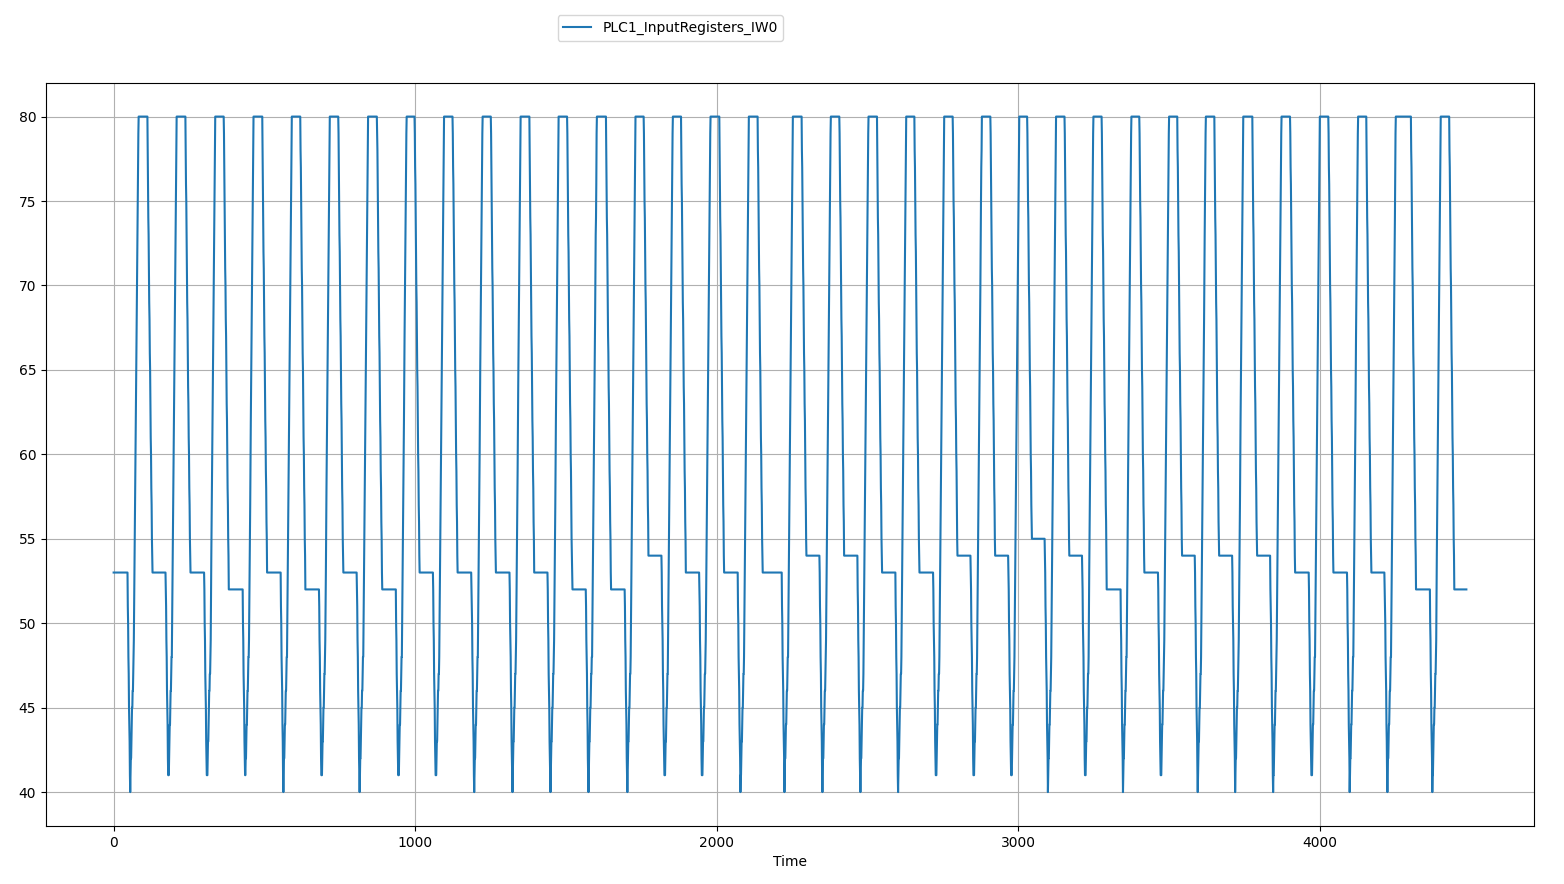
\includegraphics[width=\textwidth]{chap3/chartPlot_ceccato.png}
		\caption{Chart plot for\\ \textnormal{\texttt{PLC1\_InputRegisters\_IW01}} register}
		\label{subfig:chart_plot_ceccato}
	\end{subfigure}
	\hfill
	\begin{subfigure}{0.48\textwidth}
		\includegraphics[width=\textwidth]{chap3/histPlot_ceccato.png}
		\caption{Histogram plot for\\ \textnormal{\texttt{PLC1\_InputRegisters\_IW01}} register}
		\label{subfig:hist_plot_ceccato}
	\end{subfigure}
	\caption{Output graphs from graph analysis}
	\label{fig:ceccato_graphs}
\end{figure}

The first script plots the charts, one at the time, of certain registers entered by the user from the command line, plots in which one can see the trend of the data and get a first basic idea of what that particular register contains (a measurement, an actuation, a hardcoded setpoint, ...) and possibly the trend; the second script, instead, shows \textbf{a histogram and statistical informations} about the register entered as command-line input. These informations include:

\begin{itemize}
	\item the mean, median, standard deviation, maximum value and minimum value
	
	\item two tests for the statistical distribution: \textit{Chi-squared} test for uniformity and \textit{Shapiro-Wilk} test for normality, as shown in Listing \ref{lst:stats_anal}:

\end{itemize}

\begin{lstlisting}[language=Python,numbers=none,caption={Statistical data for \textnormal{\texttt{PLC1\_InputRegisters\_IW0}} register},label=lst:stats_anal]
	Chi-squared test for uniformity
	Distance      pvalue    Uniform?
	12488.340   0.00000000    NO    
	
	Shapiro-Wilk test for normality
	Test statistic    pvalue    Normal? 
	0.844   0.00000000    NO    
	
	Stats of PLC1_InputRegisters_IW0
	Sample mean = 60.8881; Stddev = 13.0164; max = 80; min = 40 for 4488 values
\end{lstlisting}

\subsection{Invariants Inference and Analysis}
\label{subsec:ceccato_invariants}
For invariant analysis Ceccato et al. rely on \textbf{Daikon} \cite{daikon_site}, a framework to \textbf{dynamically detect likely invariants} within a program. An \textit{invariant} is a property that holds at one or more points in a program, properties that are not normally made explicit in the code, but within assert statements, documentation and formal specifications: invariants are useful in understanding the behavior of a program (in our case, of the cyber physical system).

Daikon uses \textit{machine learning} techniques applied to arbitrary data with the possibility of setting custom conditions for analysis by using a specific file \cite{daikon_spinfo} with a \textit{.spinfo} extension (see Listing \ref{lst:spinfo}). The framework is designed to find the invariants of a program, with various supported programming languages, starting from the direct execution of the program itself or passing as input the execution run (typically a file in CSV format): the authors of the paper tried to apply it by analogy also to the execution runs of a cyber physical system, to extract the invariants of this system.

\begin{lstlisting}[language=Python,numbers=none,caption={Generic example of a .spinfo file for customizing rules in Daikon},label=lst:spinfo]
	PPT_NAME aprogram.point:::POINT
	VAR1 > VAR2
	VAR1 == VAR3 && VAR1 != VAR4
\end{lstlisting}

Therefore, Daikon is fed with the no-timestamp enriched dataset obtained in the pre-processing phase (in the paper, the timestamped dataset is erroneously mentioned as input): a simple bash script launches Daikon (optionally specifying the desired condition for analysis in the \textit{.spinfo} file), which output is simply redirected to a text file containing the general invariants of the system (i.e., valid regardless of any custom condition specified), those generated based on the custom condition in the \textit{.spinfo} file, and those generated based on the negation of the condition. When the analysis is finished, the user is asked to enter the name of a registry to view its related invariants.\newline \newline
Some examples of invariants derived from the enriched dataset may be:

\begin{itemize}
	\item measurements bounded by some setpoint
	
	\item Actuators state changes occourred in the proximity of setpoints or, vice versa, proximity of setpoints upon the occurrence of a regular actuator state change
	
	\item state invariants of some actuator correspond to a specific trend in the evolution of the measurement (ascending, descending, or stable) or, vice versa, the measurement trend corresponds to a specific state invariant of some actuator
\end{itemize}

\subsection{Businness Process Mining and Analysis}
\label{subsec:ceccato_businessprocess}
\textit{Process mining} is the analysis of operational processes based on the event log \cite{process_mining_def}: the aim of this analysis is to \textbf{extract useful informations} from the event data to \textbf{reconstruct and understand the behavior} of the business process and how it was actually performed.

\bigskip
Process mining for the system under consideration starts from the event logs obtained from scanning the memory registers of the PLCs and sniffing the network communications related to the Modbus protocol, described in Subsection \ref{subsec:ceccato_scan} and representing the \textit{execution trace} of the system: through a Java program, information is extracted and combined from these event logs, and the result saved in a CSV format file.

This file is fed to \textbf{Disco} \cite{disco}, a commercial process mining tool, which generates an \textit{activity diagram} similar to UML Activity Diagram and whose nodes represent the activities while the edges represent the relations between these activities: in Figure \ref{fig:disco_example} we can see an example of this diagram referred to PLC2 of the testbed.

\begin{figure}[ht]
	\centering
	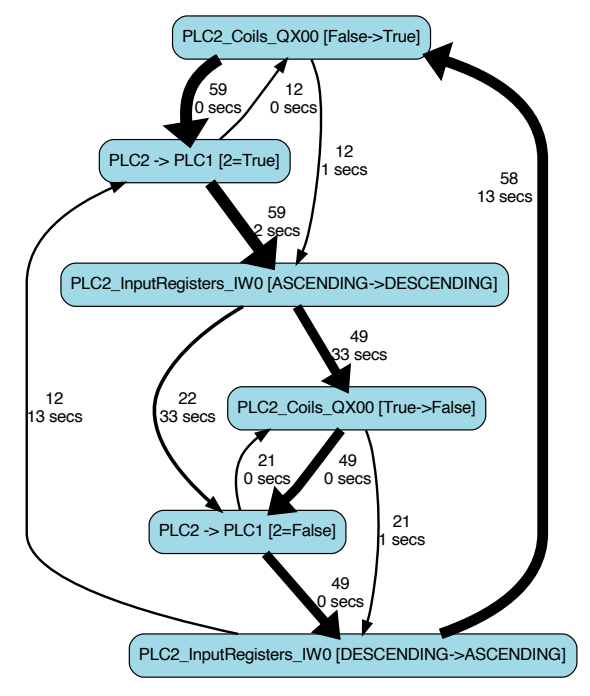
\includegraphics[scale=0.30]{chap3/disco_example.png}
	\caption{An example of Disco generated activity diagram for PLC2}
	\label{fig:disco_example}
\end{figure}

The \textit{business process} obtained in this way provides an \textbf{overview of the system} and makes it possible to \textbf{make conjectures} about its behavior, particularly between changes in actuator state and measurement trends (i.e., a given change in state of some actuators corresponds to a specific measurement trend and vice versa), and with the possibility of \textbf{establishing causality} between Modbus communications and state changes within the physical system.

\subsection{Application}
\label{subsec:ceccato_application}
In this section we will see how the black box analysis presented above in its various phases is applied in practice, using the testbed described in Subsection \ref{subsec:ceccato_testbed}.
The methodology supports a \textbf{\textit{top-down} approach}: that is, we start with an overview of the industrial process and then gradually refine our understanding of the process by descending to a higher and higher level of detail based on the results of the previous analyses and focusing on the most interesting parts of the system for further in-depth analysis.

\paragraph{Data Collection and Pre-processing} 
According to what is described in the paper, the data gathering process lasted six hours, with a granularity of one data point per second (a full system cycle takes approximately 30 minutes). Each datapoint consists of 168 attributes (55 registers plus a special register concerning the tank slope of each PLC) after the enrichment. In addition, IP addresses are automatically replaced by an abstract name identified by the prefix PLC followed by a progressive integer (PLC1, PLC2, PLC3), in order to make reading easier.

\paragraph{Graphs and Statistical Analysis}
It is unclear from the paper where exactly the information that follows was derived (graph analysis? Statistical analysis? Human reading of the dataset?), however, three properties about the contents of the registers were discovered: 

\begin{description}
	\item[\colorbox{backcolourtext}{\textnormal{\textit{Property 1:}}}] \texttt{PLC1\_MemoryRegisters\_MW0},  \texttt{PLC1\_MemoryRegisters\_MW1}, \\ \texttt{PLC2\_MemoryRegisters\_MW0},  \texttt{PLC2\_MemoryRegisters\_MW1}, \\ 
	\texttt{PLC3\_MemoryRegisters\_MW0} and 
	\texttt{PLC3\_MemoryRegisters\_MW1}
 
	registers contain constant integer values (40, 80, 10, 20, 0, 10 respectively)\footnote{From my tests on the original tool and dataset, the \texttt{PLC3\_MemoryRegisters\_MW0} register is deleted during the \textit{pre-processing} phase, as it is recognized as an unused register because of the constant value "0" it takes on. This leads me to assume that the properties are derived from a human read of the dataset prior to the \textit{pre-processing} phase.}. We may speculate that they may be (relative) hardcoded \textbf{setpoints}.
	
	\item[\colorbox{backcolourtext}{\textnormal{\textit{Property 2:}}}] \texttt{PLC1\_Coils\_QX01}, \texttt{PLC1\_Coils\_QX02}, \texttt{PLC2\_Coils\_QX01}, \\ \texttt{PLC2\_Coils\_QX02}, \texttt{PLC3\_Coils\_QX01} and \texttt{PLC3\_Coils\_QX03} contain mutable binary (Boolean) values.
	We can assume that these registers can be associated with the \textbf{actuators} of the system.
	
	\item[\colorbox{backcolourtext}{\textnormal{\textit{Property 3:}}}] \texttt{PLC1\_InputRegisters\_IW0},
	\texttt{PLC2\_InputRegisters\_IW0} and \\ \texttt{PLC3\_InputRegisters\_IW0} registers contain mutable values.
\end{description}

\textit{Property 3} suggests that those registers might contain \textbf{values related to measurements}: it is therefore necessary to investigate further to see if the conjecture (referred to as \textit{Conjecture 1} in the paper) is correct.

\begin{figure}[ht]
	\centering
	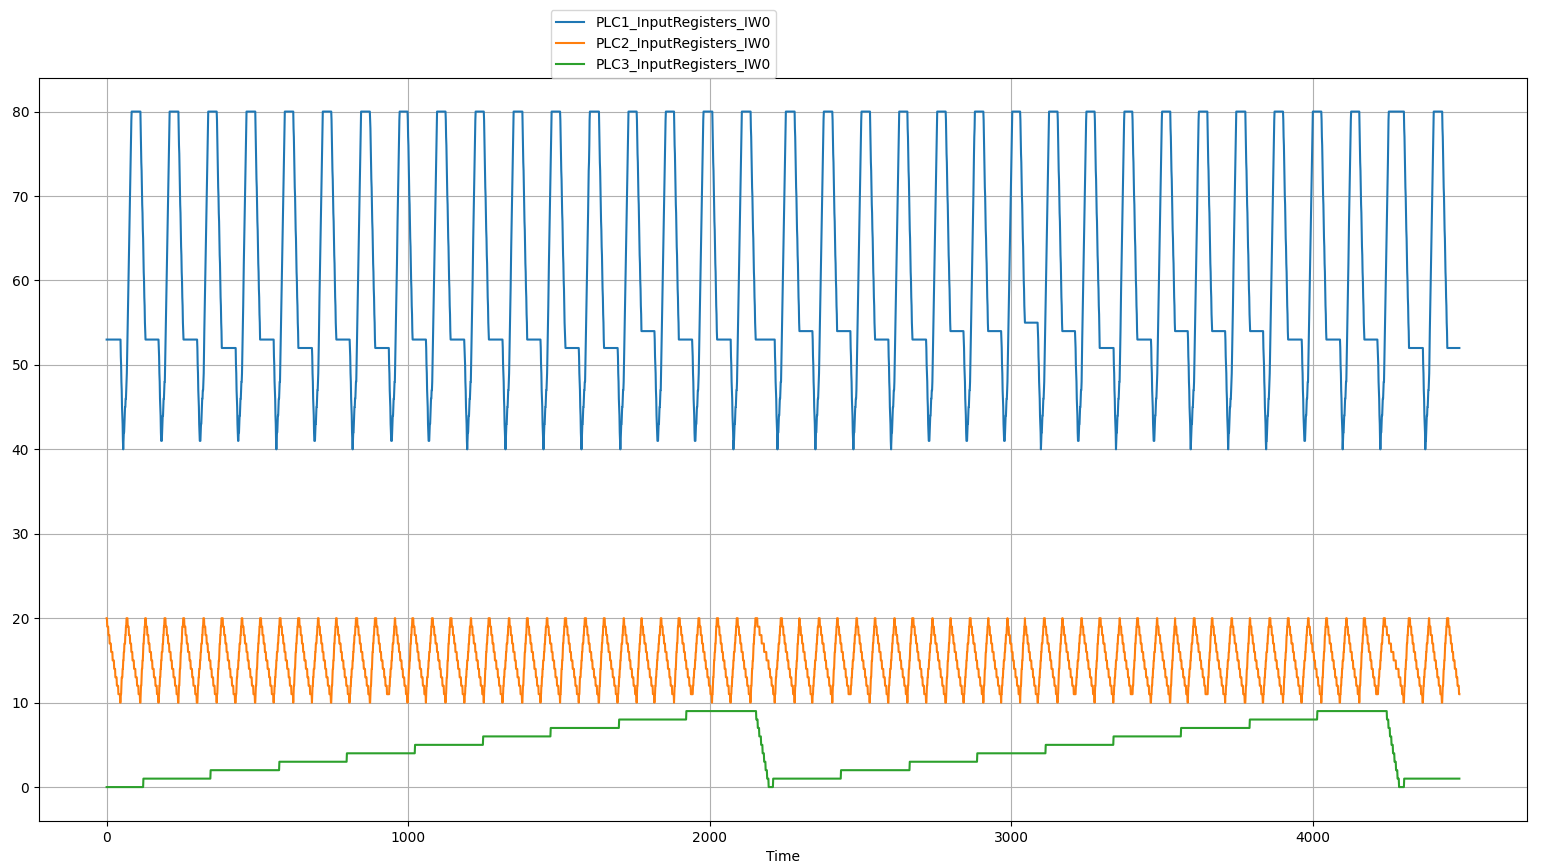
\includegraphics[scale=0.30]{chap3/graph_analysis_prop3_ceccato.png}
	\caption{Execution traces of InputRegisters\_IW0 on the three PLCs}
	\label{fig:graph_analysis_prop3}
\end{figure}

The graph analysis of the \texttt{InputRegisters\_IW0} registers of the three PLCs (summarized in Figure \ref{fig:graph_analysis_prop3} with a single plot) not only seems to confirm the conjecture, but also allows the measurements to be correlated with the contents of the \texttt{MemoryRegisters\_MW0} and \texttt{MemoryRegisters\_MW1} registers to the measurements, which represent the \textbf{relative setpoints of the measurements}.\\
Hence, we have \textit{Conjecture 2} described in the paper referring to the relative setpoints:\newline \newline
\colorbox{backcolourtext}{\emph{Conjecture 2:}} 

	- 40 and 80 are the relative setpoints for \texttt{PLC1\_InputRegisters\_IW0}
	
	- 10 and 20 are the relative setpoints for \texttt{PLC2\_InputRegisters\_IW0}
	
	- 0 and 9 are the relative setpoints for \texttt{PLC3\_InputRegisters\_IW0} 

\bigskip
Further confirmation of this conjecture may come from statistical analysis. Indeed, in the example in Listing 3.1, some statistical data are given for the register \texttt{PLC1\_InputRegisters\_IW0}, including the maximum value and the minimum value: these values are, in fact, 80 and 40 respectively.

\paragraph{Business Process Mining and Analysis}
With Business Process Mining, the authors aim to \textbf{visualize and highlight relevant system behaviors} by relating PLC states and Modbus commands.

\bigskip
Through analysis of the activity diagrams shown in Figure \ref{fig:business_process_cecccato}, drawn through Disco, we derive the following properties and conjectures:

\begin{description}
	\item[\colorbox{backcolourtext}{\textnormal{\textit{Property 4:}}}] PLC2 sends messages to PLC1 (see Figure \ref{subfig:pm_plc2}) which are recorded to \texttt{PLC1\_Coils\_QX02}.
	
	\item[\colorbox{backcolourtext}{\textnormal{\textit{Conjecture 3:}}}] \texttt{PLC2\_Coils\_QX00} determines the trend in tank T-202 (Figure \ref{subfig:pm_plc2}). \newline
	When this register is set to \textit{True}, the input register \texttt{PLC2\_InputRegisters\_IW0} related to the tank controlled by PLC2 starts an \textbf{ascending trend}; vice versa, when the coil register is set to \textit{False}, the input register starts a \textbf{descending trend}.
	
	\item[\colorbox{backcolourtext}{\textnormal{\textit{Conjecture 4:}}}] If \texttt{PLC1\_Coils\_QX00} change his value to True, trend in tank T-201, related to \texttt{PLC1\_InputRegisters\_IW0} and controlled by PLC1, become \textbf{ascending} (see Figure \ref{subfig:pm_plc1})

	\item[\colorbox{backcolourtext}{\textnormal{\textit{Conjecture 5:}}}] \texttt{PLC3\_Coils\_QX00} starts a \textbf{decreasing trend} in tank T-203, related to \texttt{PLC3\_InputRegisters\_IW0} and controlled by PLC3, whereas \texttt{PLC3\_Coils\_QX02} starts an \textbf{increasing trend} on the tank (see Figure \ref{subfig:pm_plc3})
\end{description}
\vfill
\pagebreak

\begin{figure}[H]
	\centering
	\begin{subfigure}{0.7\textwidth}
		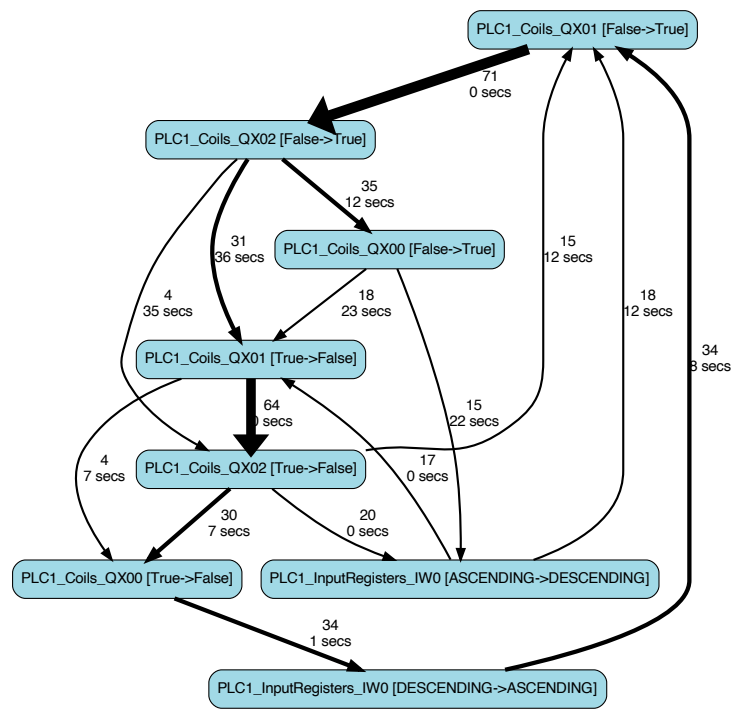
\includegraphics[width=\textwidth]{chap3/disco_plc1.png}
		\caption{States in PLC1}
		\label{subfig:pm_plc1}
	\end{subfigure}
	\hfill
	\begin{subfigure}{0.48\textwidth}
		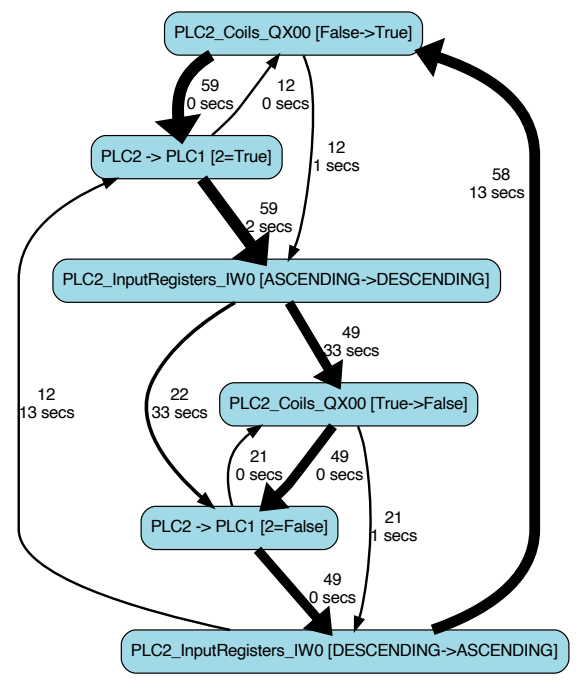
\includegraphics[width=\textwidth]{chap3/disco_plc2.png}
		\caption{States and Modbus command in PLC2}
		\label{subfig:pm_plc2}
	\end{subfigure}
	\hfill
	\begin{subfigure}{0.48\textwidth}
		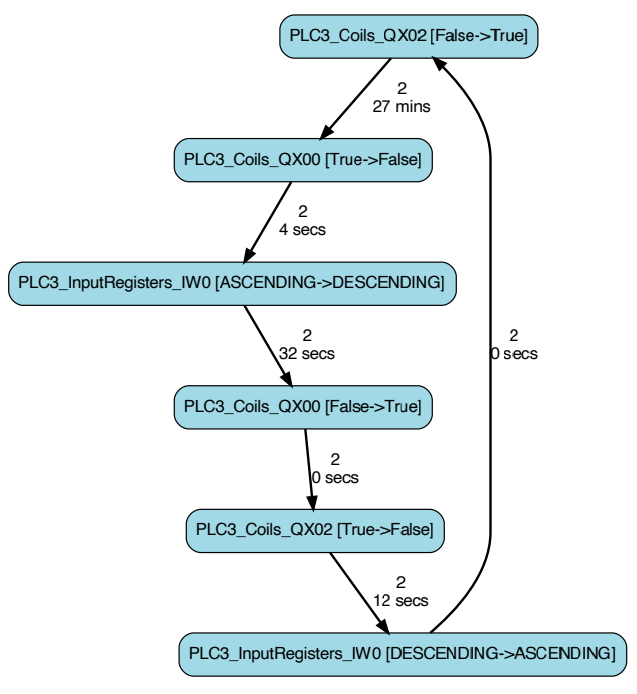
\includegraphics[width=\textwidth]{chap3/disco_plc3.png}
		\caption{States in PLC3}
		\label{subfig:pm_plc3}
	\end{subfigure}
	\caption{Business process with states and Modbus commands for the three PLCs}
	\label{fig:business_process_cecccato}
\end{figure}

\paragraph{Invariants Inference and Analysis}
The last phase of the analysis of the example industrial system is invariant analysis, performed through Daikon framework. At this stage, an attempt will be made to confirm what has been seen previously and to derive new properties of the system based on the results of the Daikon analysis.

\bigskip
To get gradually more and more accurate results, the authors presumably performed more than one analysis with Daikon, including certain rules within the \textit{splitter information file} (see Section \ref{subsec:ceccato_invariants} and Listing \ref{lst:spinfo}) based on specific conditions placed on the measurements, for example, the level of water contained in a tank. Given moreover the massive amount of invariants generated by Daikon's output, it is not easy to identify and correlate those that are actually useful for analysis: this must be done manually.

\bigskip
However, it was possible to have confirmation of the conjectures made in the previous stages of the analysis: starting with the setpoints, analyzing the output of the invariants returned by Daikon\footnote{The invariants shown here are a manual summary and derivation of those actually returned in output by Daikon. I will discuss this more in Section \ref{subsec:ceccato_limitations}} reveals that \newline \newline
\small\texttt{PLC1\_InputRegisters\_IW0 >= PLC1\_MemoryRegisters\_MW0 == 40.0}\\
\texttt{PLC1\_InputRegisters\_IW0 <= PLC1\_MemoryRegisters\_MW1 == 80.0}\\
\texttt{PLC2\_InputRegisters\_IW0 >= PLC2\_MemoryRegisters\_MW0 == 10.0}\\
\texttt{PLC2\_InputRegisters\_IW0 <= PLC2\_MemoryRegisters\_MW1 == 20.0}\\
\texttt{PLC3\_InputRegisters\_IW0 >= PLC3\_MemoryRegisters\_MW0 == 0.0}\\
\texttt{PLC3\_InputRegisters\_IW0 <= PLC3\_MemoryRegisters\_MW1 == 9.0} \newline \newline
\normalsize i.e., that the \texttt{MemoryRegisters\_MW0} and \texttt{MemoryRegisters\_MW1} registers of each PLC contain the \textbf{absolute minimum and maximum setpoints}, respectively (\textit{Property 5}).

\bigskip
There is also a confirmation regarding \textit{Property 4}: from the computed invariants it can be seen that \newline \newline
\small\texttt{PLC1\_Coils\_QX01 == PLC1\_Coils\_QX02 == PLC2\_Coils\_QX00}\newline \newline
\normalsize and from this derive that there is a \textbf{communication channel between PLC2 and PLC1}, where the value of \texttt{PLC2\_Coils\_QX00} is copied to \texttt{PLC1\_Coils\_QX01} and \texttt{PLC1\_Coils\_QX02} (\textit{Property 6}).

\bigskip
Regarding the \textbf{relationships between actuator state changes and measurement trends}, invariant analysis yields the results summarized in the following rules:

\begin{description}
	\item[\colorbox{backcolourtext}{\normalfont\textit{Property 7:}}] Tank T-202 level \textit{increases} iif \texttt{PLC1\_Coils\_QX01 == True}. Otherwise, if \texttt{PLC1\_Coils\_QX01 == False} will be \textit{non-increasing}.
\end{description}
	This is because if the coil is \textit{True} the condition \newline \scriptsize\texttt{PLC2\_InputRegisters\_IW0 == PLC2\_MemoryRegisters\_MW0 == 20.0 \&\& PLC2\_slope > 0} \newline \normalsize is verified. 
	On the opposite hand, if the coil is \textit{False}, the condition \newline \scriptsize\texttt{PLC2\_InputRegisters\_IW0 == PLC2\_MemoryRegisters\_MW0 == 20.0 \&\& PLC2\_slope <= 0}  \normalsize is verified. The \textit{slope} is an auxiliary attribute indicating the trend of the measurement: increasing if > 0, decreasing if < 0, stable otherwise.

\begin{description}
	\item[\colorbox{backcolourtext}{\normalfont\textit{Property 8:}}] Tank T-201 level \textit{increases} iif \texttt{PLC1\_Coils\_QX00 == True}. On the other hand, if \texttt{PLC1\_Coils\_QX00 == False} and if \texttt{PLC1\_Coils\_QX01 == True} the level will be \textit{non-decreasing}.
	
	\item[\colorbox{backcolourtext}{\normalfont\textit{Property 9:}}] Tank T-203 level \textit{decreases} iif \texttt{PLC3\_Coils\_QX00 == True}. It will be \textit{non-decreasing} if \texttt{PLC1\_Coils\_QX00 == False}.
\end{description}

The last two properties concern the \textbf{relationship between actuator state changes and the setpoints}: it is intended to check what happens to the actuators when the water level reaches one of these setpoints. From the analysis of the relevant invariants, the following properties are derived:

\begin{description}
	\item[\colorbox{backcolourtext}{\normalfont\textit{Property 10:}}] Tank T-201 reaches the upper absolute setpoint when\\ \texttt{PLC1\_Coils\_QX00} changes its state from \textit{True} to \textit{False}. If the coil changes from \textit{False} to \textit{True}, the tank reaches its absolute lower setpoint.
	
	\item[\colorbox{backcolourtext}{\normalfont\textit{Property 11:}}]
	Tank T-203 reaches the upper absolute setpoint when\\ \texttt{PLC3\_Coils\_QX00} changes its state from \textit{True} to \textit{False}. If the coil changes from \textit{False} to \textit{True}, the tank reaches its absolute lower setpoint.	 
\end{description}

\subsection{Limitations}
\label{subsec:ceccato_limitations}
The methodology proposed by Ceccato et al. is certainly valid and offers a good starting point for approaching the reverse engineering of an industrial control system from the attacker's perspective, while also providing a tool to perform this task.

\bigskip
The limitations of this approach, however, all lie in the tool mentioned above and also in the testbed described in Section \ref{subsec:ceccato_testbed}. In this section I will explain which are the criticisms of each phase, while in Chapter 4 I will formulate proposals to improve and make this methodology more efficient.

\paragraph{General Criticism}
\label{par:limit_ceccato_general}
The general critical aspects of the application of this approach are many: the primary one concerns the fact that the proposed tool seems to be built specifically for the testbed used and that it is not applicable to other contexts, even to the same type of industrial control system (water treatment systems, in this case). 

\bigskip
What severely limits the analysis performed with the tool implemented by Ceccato et al. is the use of \textit{ad hoc} solutions and \textit{a posteriori} interventions done manually on the datasets after the data gathering process: I will discuss this last aspect in more detail later.\newline
Moreover, there is the presence of many \textit{hardcoded} variables and conditions within the scripts: this makes the system unconfigurable and unable to properly perform the various stages of the analysis as errors can occur due to incorrect data and mismatches with the system under analysis.

Having considered, furthermore, only the Modbus protocol for network communications between the PLCs is another major limiting factor and does not help the methodology to be adaptable to different systems communicating with different protocols (sometimes even multiple ones on the same system). 

\bigskip
Let us now look at the limitations and critical aspects of each phase.

\paragraph{Testbed}
\label{par:limit_ceccato_testbed}
The testbed environment used by Ceccato et. al is entirely simulated, from the physical system to the control system. The PLCs were built with \textbf{OpenPLC} \cite{openplc} in a Docker environment \cite{docker}, while the physics part was built through \textbf{Simulink} \cite{simulink}.

\bigskip
OpenPLC is an open source cross-platform software that simulates the hardware and software functionality of a physical PLC and also offers a complete editor for PLC program development with support for all standard languages: \textit{Ladder Logic} (LD), \textit{Function Block Diagram} (FBD), \textit{Instruction List} (IL), \textit{Structured Text} (ST), and \textit{Sequential Function Chart} (SFC).\newline
It is for sure an excellent choice for creating a zero-cost industrial or home automation and \textit{Internet of Things} (IoT) system that is easy to manage via a dedicated, comprehensive and functional web interface. In spite of these undoubted merits, however, there are (at the moment) \textbf{very few supported protocols}: the main one and also referred to in the official documentation is \textbf{Modbus}, while the other protocol is DNP3.

\bigskip
The biggest problem with the testbed, however, is not with the controller part, but with the \textbf{physical part}: first of all, it must be said that although this is something purely demonstrative even though it is fully functional, the implemented Simulink model is really \textbf{oversimplified} compared to the iTrust SWaT system, which itself is a scaled-down version of a real water treatment plant. In fact, in the entire system there are only three actuators, two of which are connected to the same tank and controlled by the same PLC, and sensors related only to the water level in the system's tanks: in a real system there are many more \textit{field devices}, which can monitor and control other aspects of the system beyond the mere contents of the tanks. Consider, for example, measuring and controlling the chemicals in the water, the pressure of the liquid in the filter unit, or more simply the amount of water flow at a given point or time.\newline
All these must be considered and represent a number of additional variables that makes analysis and consequently reverse engineering of the system more difficult.

\bigskip
The second critical aspect concerns the \textbf{simulation of the physics of the liquid} inside the tanks: Simulink does not consider the fact that inside a tank that is filling (emptying) the liquid in it undergoes \textbf{fluctuations} which cause the level sensor not to see the water level constantly increasing (decreasing) or at most being stable at each point of detection. Figure \ref{fig:testbed_physics} exemplifies more clearly with an example the concept just expressed: these oscillations cause a \textbf{perturbation} in the data.\newline
This issue leads to the difficulty, on a real physical system, of \textbf{correctly calculating the trend of a measurement} by using the slope attribute: if this was obtained with a too low granularity, the trend will be oscillating between increasing and decreasing even when in reality this would be in general increasing (decreasing) or stable; on the other hand, if the slope was obtained with a too high granularity there is a loss of information and the trend may be "flattened" with respect to reality.\newline
In the present case, the slope in the Simulink model was calculated statically \textit{point-to-point}, thus with a granularity of one second: an averagely careful reader will have already guessed that this granularity is inapplicable to the real system in Figure \ref{subfig:real_physics}. As we will later see, we need to \textbf{operate on the data perturbations} to be able to obtain a suitable granularity and a correct calculation of the slope and consequently of the measurement trend.
\vfill

\pagebreak
\begin{figure}[ht]
	\centering
	\begin{subfigure}{0.9\textwidth}
		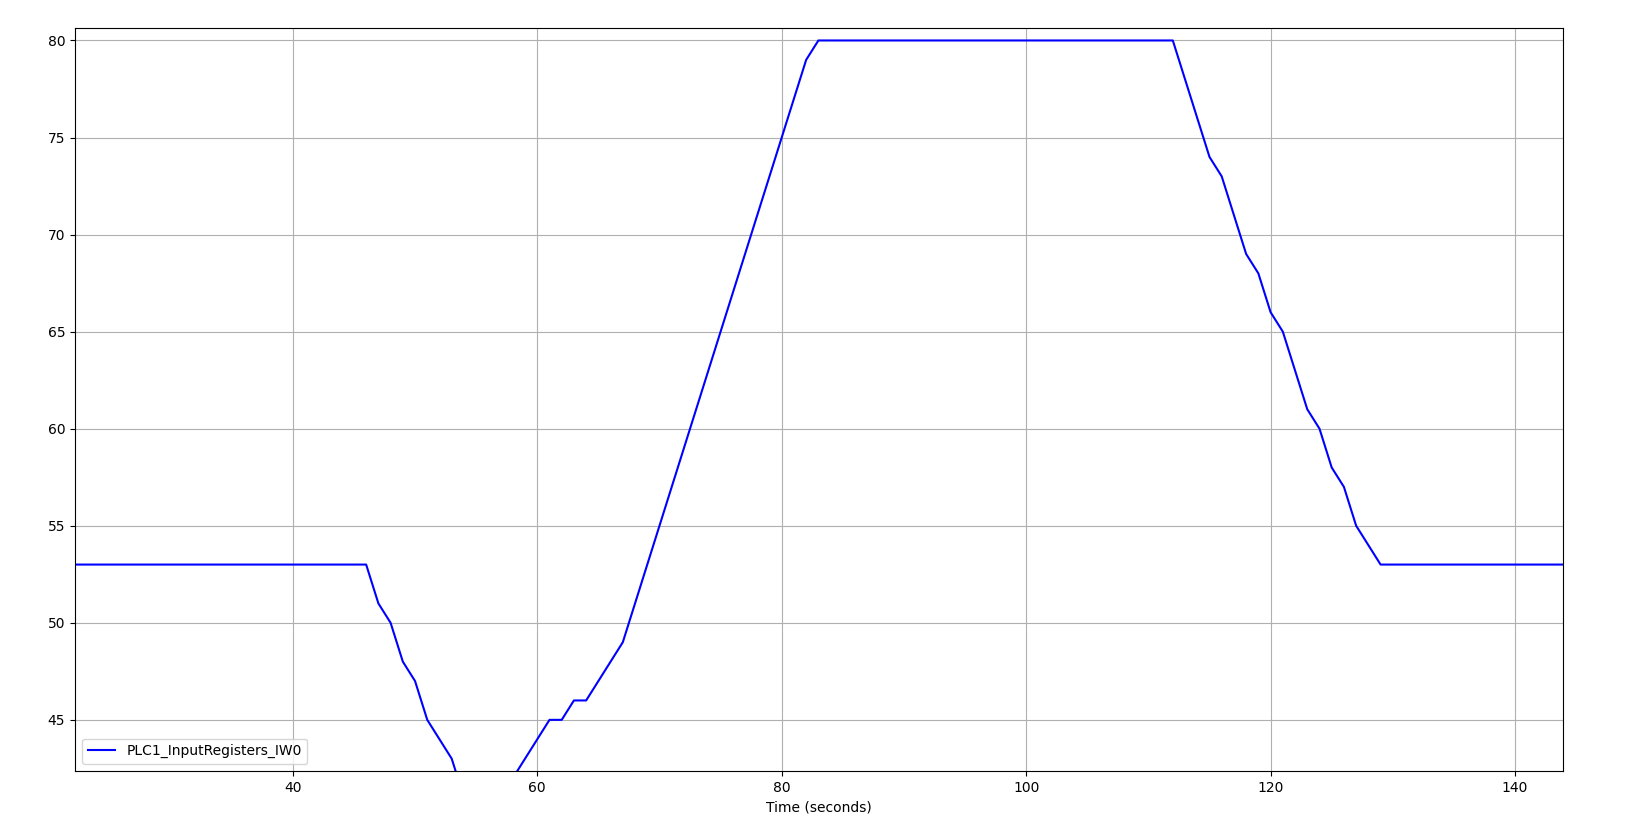
\includegraphics[width=\textwidth]{chap3/simulink_physics.png}
		\caption{}
		\label{subfig:simulink_physics}
	\end{subfigure}
	\hfill
	\begin{subfigure}{0.9\textwidth}
		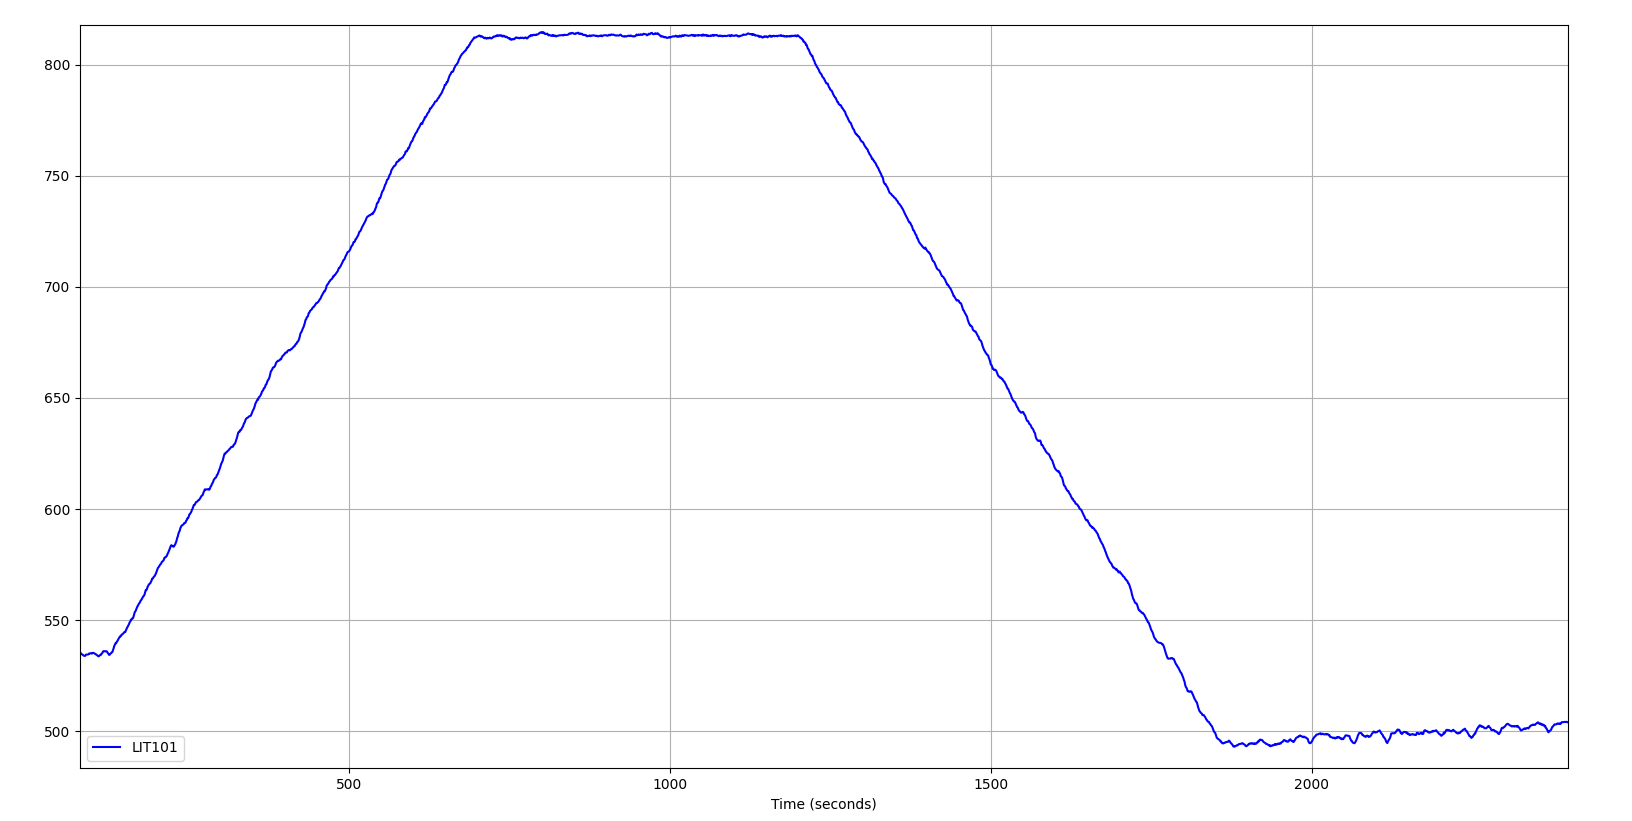
\includegraphics[width=\textwidth]{chap3/real_physics.png}
		\caption{}
		\label{subfig:real_physics}
	\end{subfigure}
	\caption{Water physics compared: simulated physics in the Simulink model (a) and physics in a real system (iTrust SWaT) (b). Fluctuations in the tank level in (b), almost completely absent in (a), can be appreciated.}
	\label{fig:testbed_physics}
\end{figure}

\paragraph{Pre-processing}
In the pre-processing phase, the authors make use of a Python script to merge all the datasets of the individual PLCs into a single dataset, remove the (supposedly) unused registers, and finally enrich the obtained dataset with additional attributes. These attributes are:

\begin{itemize}
	\item the previous value of all registers
	
	\item some additional relative setpoints named \texttt{PLC\textit{x}\_Max\_safety} and\\ 
	\texttt{PLC\textit{x}\_Min\_safety} (where \textit{x} is the PLC number), which represent a kind of alert on reaching the maximum and minimum water levels of the tanks
	
	\item the measurement slope, that is, the trend of the water level in the system tanks along the system cycles.	
\end{itemize}

Merging the datasets of all individual PLCs into a single dataset representing the entire system can be a sound practice if the system to be anlized is (very) small as is the testbed analyzed here, consisting of a few PLCs and especially a few registers. If, however, the complexity of the system increases, this type of merging can become counterproductive and make it difficult to analyze and understand the data obtained in subsequent steps.\newline 
In short, there is no possibility to analyze only a subsystem and thus make the analysis faster and more understandable. Moreover, a data gathering can take up to days, and the analyst/attacker may need to make an analysis of the system isolating a precise time range, ignoring everything that happens before and/or after: all of this, with the tool we have seen, cannot be done.

\bigskip
Regarding the additional attributes, looking at the code of the script that performs the enrichment, I observed that \textbf{some attributes were manually inserted} after the merging phase: I am referring in particular to the attributes \texttt{PLC\textit{x}\_Max\_safety} and \texttt{PLC\textit{x}\_Min\_safety}, whose references were moreover hardcoded into the script, and the \textit{slope} whose calculation method I mentioned in the previous paragraph about the testbed limitations.\newline
In the end, only the attribute \textit{prev} related to the value at the previous point of the detection is inserted automatically for all registers, moreover without the possibility to choose whether this attribute should be extended to all registers or only to a part.

\paragraph{Graphs and Statistical Analysis}
Describing the behavior of graphical analysis in Section \ref{subsec:ceccato_graphanalysis} I had already mentioned that only one register plot at a time was shown and not, for example, a single window containing the charts of all registers entered by the user as input from the command line, such as in Figure \ref{fig:graph_analysis_prop3}.\newline
While displaying charts for individual registers still provides useful information about the system such as the distinction between actuators and measurements and the general trend of the latter, single display does not allow one to catch, or at least makes it difficult, the relationship that exists between actuators and measurements, where it exists, because a view of the system as a whole is missing.\\
In this way, the risk is to make conjectures about the behavior of the system that may prove to be at least imprecises, if not inaccurates.

\bigskip
On the other hand, regarding the statistical analysis, two observations need to be made: the first is that for the given system, I personally was unable to appreciate the usefulness of the generated histogram, as it does not provide any particular new information that has not already been obtained from the graphical analysis (except maybe something marginal); the second observation is that precisely the plot of the histogram "hides" the statistical informations obtained: these are in fact shown on the terminal from which the script is launched, but to an uncareful eye or one unfamiliar with the script's behavior they can easily be interpreted as simple debugging output, since at the same time the window containing the histogram plot is shown. In general, however, little statistical information is provided.

\paragraph{Business Process Mining and Analysis}
Concerning the data mining, this is a purely ad \textit{hoc solution}, designed to work under special conditions: first, the timestamped dataset of the physical process and the one obtained after the packet sniffing operation of Modbus traffic on the network need to be synchronized and have the same granularity, in this case one event per second.\newline
It is relatively easy, therefore, to find correspondences between Modbus commands sent over the network and events occurring on the physical system, such as state changes in actuations, due in part to the fact that the number of communications over the network is really small (see Section \ref{subsec:ceccato_testbed}). In a real system, network communications are much more numerous and involve many more devices even in the same second: finding the exact correspondence with what is happening in the cyber physical system becomes much more difficult.

\bigskip
Since this is, as mentioned, an \textit{ad hoc} solution, only the Modbus protocol is being considered: as widely used as this industrial protocol is, other protocols that are widely used such as EtherNet/IP (see Section \ref{subsub:enip}) should be considered in order to extend the analysis to other industrial systems that use a different communication network.

\bigskip
The other limiting aspect of the business process mining phase is the \textbf{process mining software} used to generate the activity diagram. As mentioned in Section \ref{subsec:ceccato_businessprocess}, the process mining software used by Ceccato et al. is \textbf{Disco}: this is commercial software, with an academic license lasting only 30 days (although free of charge), released for Windows and MacOS operating systems only, which makes its use under Linux systems impossible except by using emulation environments such as Wine.\newline
For what is my vision and training as a computer scientist, it would have been preferable to use a \textit{cross-platform}, \textit{freely licensed open source} software alternative to Disco: one such software could have been \textbf{ProM Tools} \cite{prom_tools}, a framework for process mining very similar to Disco in functionality, but fitting the criteria just described, or use Python libraries such as \textbf{PM4PY} \cite{pm4py}, which offer ready-to-use algorithms suitable for various process mining needs.

\paragraph{Invariants Inference and Analysis}
The limitation in this case is principally Daikon: this software is designed to compute the invariants of a software from its live execution or from a file containing its execution flow, not to find the invariants of a cyber physical system. Since there are currently no better consolidated alternatives for inferring invariants, however, an attempt was still made to use Daikon as best as possible.

\begin{figure}[H]
	\centering
	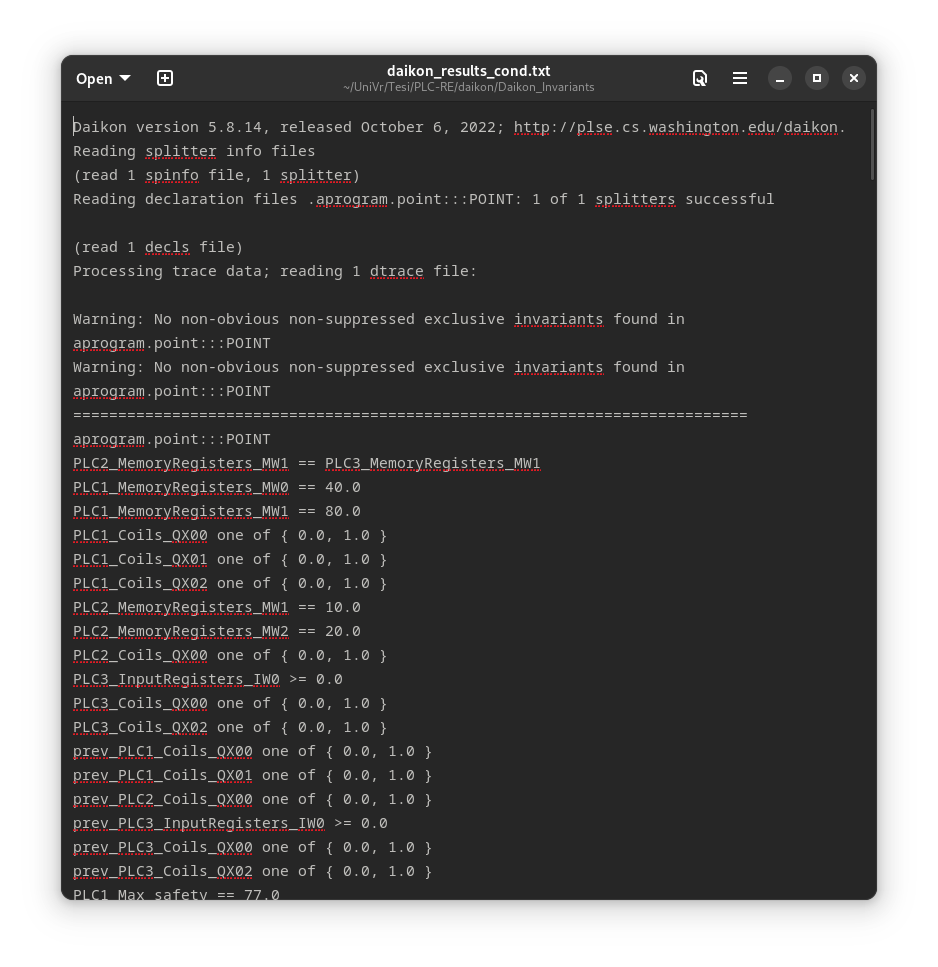
\includegraphics[scale=0.35]{chap3/daikon_output_ceccato.png}
	\caption{Example of Daikon's output}
	\label{fig:daikon_output_ceccato}
\end{figure}

The biggest problem with Daikon applied to the computation of invariants of an industrial system is the difficult reading of the resulting output: the software in fact returns a very long list of invariants, one invariant per line, many of no use and without correlating invariants that may have common features or deriving additional information from them. The process of screening and recognizing the significant invariants, as well as the correlation between them, must be done by a human: certainly not an easy task given the volume of invariants one could theoretically be faced with (hundreds and hundreds of invariants). An example of Daikon's output can be seen in Figure \ref{fig:daikon_output_ceccato}.

\bigskip
The bash script used in this phase of the analysis does not help at all in deriving significant invariants more easily: it merely launches Daikon and saves its output to a text file by simply redirecting the stdout to file. No data reprocessing is done during this step. In addition, if a condition is to be specified to Daikon before performing the analysis, it is necessary each time to edit the .spinfo file by manually entering the desired rule, an inconvenient operation when multiple analyses are to be performed with different conditions each time. 

\vfill
\nolinenumbers


%###### CAPITOLO 4 ######%
\chapter{A Substantial Improvement to Ceccato et al.’s Framework}
\label{chap:proposal}

\linenumbers
\lettrine[lines=2]{I}{n Chapter \ref{state_of_art}}, we presented the state of the art of \textit{process comprehension} of an Industrial Control System (ICS) with a focus on the methodology proposed by Ceccato et al. \cite{ceccato}[Section \ref{sec:3_ceccato_metodology}], explaining what it consists of, its practical application on a testbed, and most importantly highlighting its limitations and critical issues (see Section \ref{subsec:3_ceccato_limitations}).

\bigskip
In this chapter we will present \textbf{a proposal to improve the methodology} presented in the previous chapter, addressing most of the critical issues (or at least trying to do so) mentioned above by almost completely rewriting the original framework, enhancing its functionalities and inserting new ones where possible, while preserving its general structure and approach. The system analysis will in fact consist of the same four steps as in the original methodology (Data Pre-processing, Graph and Statistical Analysis, Business Process Mining and Invariants Inference), but each of them will be deeply revised in order to provide a richer, clearer and more complete process comprehension of the industrial system to be analyzed and its behavior.

\bigskip
As it may have already been noted, my proposals do not involve improving the data gathering phase: this is due simply to the fact that the novel framework will not be tested on the same case study used by Ceccato et, al. (Section \ref{subsec:3_testbed}), but on a different case study, the ITrust SWaT system \cite{swat_home}, of which (some) datasets containing the execution trace of the physical system and the network traffic scan are already provided by iTrust itself. For more details about this case study, the reader is referred to Chapter \ref{casestudy}.

\section{The Proposed New Framework}
\label{sec:4_framework_presentation}
In our version of the framework we decided to follow a few design choices:

\begin{enumerate}
	\item it must be implemented in a \textbf{single programming language};
	\item it must be \textbf{independent of the system} to be analyzed;
	\item It must provide greater \textbf{flexibility and ease of use} for the user at every stage.
\end{enumerate}
In the following, we discuss these three features in more detail.

\begin{description}
	\item[Single Programming Language] The original tool was implemented using various programming languages in each of the different phases: from Python up to Java, passing through Bash scripting. \newline
	In our opinion, this heterogeneity makes it more difficult and less intuitive for the user to operate on the tool: moreover, the use of multiple technologies makes it more difficult to maintain the code and add new features, particularly if only a single person is managing the code (he/she might be proficient in one language, but little of the others).
	
	\bigskip
	For these reasons, we decided to use a single programming language, to ensure homogeneity to the framework and ease of use and maintenance of the code for anyone who wants to manage it in the future: we chose to use Python, because of its simplicity and easy readability combined with its versatility and powerfulness: moreover, Python can count on a massive number of available libraries and packages that meet all kinds of needs.
	
	\item[System Independence] One of the biggest limitations of Ceccato et al.'s tool that we highlighted in Section \ref{subsec:3_ceccato_limitations} is the fact that it is \textbf{highly dependent on the testbed used}: that is, it is \textit{not} possible to configure any of the tool's parameters to analyze different industrial systems.\newline
	To overcome this issue and make my framework independent of the system to be analyzed, also eliminating all references to hardcoded variables and values present in the previous tool, we decided to use a \textbf{general configuration file}, named \textit{config.ini}, in which the user can, at will, customize all the parameters necessary to perform the analysis of the targeted system.
	
	\item[Flexibility and Ease on Use] The lack of flexibility and ease of use in a tool can be a significant disadvantage, limiting its effectiveness and making it challenging for the user to get the desired outcomes. The original tool suffered from these limitations, with users having to run scripts from the command line, with little to no options or parameters available to customize the analysis. As a result, the tool was not user-friendly and lacked the flexibility to adapt to specific user needs. 
	
	\bigskip
	To settle these issues, I enhanced the command-line interface in the novel framework by adding new options and parameters. These new features provide the user with greater flexibility, enabling to specify parameters and options that allow for more in-depth analysis and focused results analyzing data more effectively and efficiently. With these enhancements, the framework has become more user-friendly, reducing the learning curve and making it more accessible to a wider range of users. \newline
	This, in turn, makes the framework more valuable and useful, increasing its adoption and effectiveness across a range of industrial control systems and applications. \newline
	Moreover, with new options and parameters users no longer have to rely solely on the command line interface, which can be challenging and intimidating for those with limited technical expertise. Instead, users can now access a range of customizable options and parameters, making the tool more intuitive and user-friendly. 
\end{description}
Overall, the enhancements made to the framework represent a significant step forward in making it more effective, efficient, and user-friendly.


%\paragraph{General Configuration File \textit{config.ini}} 
%The configuration file \textit{config.ini} for the framework I am %presenting in this thesis is intended, as mentioned, to make it %customizable in order to fit a variety of different systems and allow 
%for their analysis. Here the user can configure general parameters and %options, such as paths to read from or write files to, or related to %individual analysis phases.\newline
%The file is divided into sections, each covering a different aspect of 
%the configuration: each section contains user-customizable constants 
%that will then be called within the Python scripts that constitute the %framework. An example can be appreciated in Listing %\ref{lst:config_ini_example}:

%\begin{lstlisting}[language=bash, numbers=none, caption=Example of %\textit{config.ini} file, label=lst:config_ini_example]	
%	[PATHS]
%	root_dir = /home/marcuzzo/UniVr/Tesi
%	project_dir = %(root_dir)s/PLC-RE
%	net_csv_path = %(root_dir)s/datasets_SWaT/2015/Network_CSV
%	
%	[PREPROC]
%	raw_dataset_directory = datasets_SWaT/2015
%	dataset_file = PLC_SWaT_Dataset.csv
%	granularity = 10
%	number_of_rows = 20000
%	skip_rows = 100000
%	
%	[DAIKON]
%	daikon_dir = daikon
%	daikon_invariants_dir = %(daikon_dir)s/Daikon_Invariants
%	daikon_results_dir = %(daikon_invariants_dir)s/results
%	daikon_results_file_original = daikon_results_full.txt
%	inv_conditions_file = Inv_conditions.spinfo
%	max_security_pct_margin = 1
%	min_security_pct_margin = 2
%	
%	...
%\end{lstlisting}

\subsection{Framework Structure}
\label{subsec:4_framework_struct}
The proposed framework follows a similar structure to the original tool, with a division into five main directories representing different phases of the analysis: \textbf{data pre-processing}, \textbf{graphs and statistical analysis}, \textbf{process mining}, and \textbf{invariant analysis}. A new phase is added compared to the original, concerning the \textbf{analysis of the network traffic}. These directories contain the corresponding Python scripts responsible for performing the analysis, along with any necessary subdirectories and input/output files to ensure the proper functioning of the framework.

\begin{lstlisting}[language=bash, numbers=none, caption=Novel Framework structure and Python scripts, label=lst:4_tree_command]
	.
	├── config.ini
	├── daikon
	│   ├── Daikon_Invariants
	│   ├── daikonAnalysis.py
	│   └── runDaikon.py
	├── network-analysis
	│   ├── data
	│   ├── networkAnalysis.py
	│   ├── export_pcap_data.py
	│   └── swat_csv_extractor.py
	├── pre-processing
	│   ├── mergeDatasets.py
	│   └── system_info.py
	├── process-mining
	│   ├── data
	│   └── process_mining.py
	└── statistical-graphs
	    ├── histPlots_Stats.py
	    └── runChartSubPlots.py
\end{lstlisting}

Ahead of these directories there is the most important part, that allows the framework to be independent of the industrial control system being analyzed: the \textit{config.ini} file. Here the user can configure general parameters and options, such as paths to read from or write files to, or related to individual analysis phases.\newline
The file is divided into sections, each covering a different aspect of 
the configuration: each section contains user-customizable parameters 
that will then be called within the Python scripts that constitute the framework. Sections of \textit{config.ini} are:

\begin{itemize}
	\item \textbf{[PATHS]:} defines general paths such as the project root directory;
	
	\item \textbf{[PREPROC]:} includes parameters needed for the \textbf{pre-processing phase}, like the directory containing the raw datasets of the individual PLCs and \textit{granularity} for the slope calculation. Granularity is the time interval over which the slope is calculated;
	
	\item \textbf{[DATASET]:} defines settings and parameters used during the \textbf{dataset enrichment} stage, for example the additional attributes;
	
	\item \textbf{[DAIKON]:} defines parameters needed for \textbf{invariant analysis} with Daikon, e.g. directories and files containing the outcomes of the analysis;
	
	\item \textbf{[MINING]:} contains parameters used during the \textbf{process mining} phase, such as data directory;
	
	\item \textbf{[NETWORK]:} includes specific settings for extracting the data obtained from the packet sniffing phase on the ICS network and converting it to CSV format. It also defines the \textbf{network protocols} that are to be analyzed.
\end{itemize}

\subsection{Python Libraries and External Tools}
\label{subsec:4_tools_libraries}
As the framework has been developed entirely in Python, the objective was to minimize reliance on external tools and instead integrate various functionalities within the framework itself. The aim was to make the framework independent from external software. The only remaining external tool from the Ceccato et al. tool is Daikon. This choice was made because there is currently no better alternative or Python package available that offers the same functionalities as Daikon.

\bigskip
Instead, the framework extensively utilizes Python libraries for handling various functionalities and input data. The core libraries on which the framework relies are:

\begin{itemize}
	\item \textbf{Pandas}, also used in the previous tool for dataset management, but whose use here has been deepened and extended	
	\item \textbf{NumPy}, often used together with Pandas to perform some operations to support it;
	
	\item \textbf{MatPlotLib}, for managing and plotting graphical analysis;
	
	\item other scientific libraries such as \textbf{SciPy}, \textbf{StatsModel} \cite{statsmodel} and \textbf{NetworkX} \cite{networkx}, for mathematical, statistical and analysis operations on the data;
	
	\item \textbf{GraphViz}, for the creation of activity diagrams in the process mining phase.
\end{itemize}
Having now seen the structure of the framework, in the next sections we will go into more detail describing our proposal.

\section{Analysis Phases}

\subsection{Phase 1: Data Pre-processing}
\label{subsec:improve_preprocessing}
\textit{Data Pre-processing phase} is probably the most delicate and significant one: depending on how large the industrial system to be analyzed is, the data collected, and how it is enriched using the additional attributes, the subsequent system analysis will provide more or less accurate outcomes.

\bigskip
The previous tool has several limitations, particularly at this stage. It does not allow for the isolation of a subsystem, either in terms of time or the number of PLCs to be analyzed. The system is considered as a whole without the ability to focus on specific subsystems. Additionally, many of the additional attributes had to be manually added, and for the ones entered automatically, there is no way to specify the register type to associate them with.\newline
The combination of these limitations, along with the presence of hardcoded references to attributes and registers in the tool's code, makes the analysis of the system more challenging. Furthermore, it compromises the accuracy and reliability of the obtained results in terms of both quantity and quality.

\bigskip
In the proposed framework, these issues have been addressed by incorporating new features. Firstly, the framework allows for the selection of a subsystem from the command line based on both temporal criteria and the specific PLCs to be included. This enables more focused and targeted analysis. Additionally, we have revamped the process of enriching the resulting dataset by eliminating manual entry of additional attributes. Instead, users now have the flexibility to determine the type of additional attribute to associate with a specific register.\newline
Furthermore, after the pre-processing stage, a preliminary analysis can be conducted on the resulting dataset. This analysis aims to identify the registers that are associated with actuators, measurements, and hardcoded setpoints or constants. It provides insights into the dataset and helps in refining the enrichment step. The parameters for this analysis can be configured in the \textit{config.ini} file, allowing for customization and fine-tuning of the process.\newline \newline 
In the upcoming sections, we will delve into a more comprehensive examination of the achievements made in this framework.
\vfill

\subsubsection{Subsystem Selection}
\label{subsubsec:4_select_subsystem}

In the previous tool, the datasets for each individual PLC in CSV format were required to be placed in a specific directory that was hardcoded in the script. The script would then merge and enrich these datasets to generate a single output dataset representing the complete process trace of the industrial system. However, the script did not provide options to select specific PLCs for analysis or define a temporal range for analysis. This lack of flexibility made the analysis more complex, especially when dealing with \textit{transient states} (i.e., general statea in which the industrial system is still initializing before actually reaching full operation) or when focusing on specific parts of the industrial system during certain periods of interest. The fixed dataset structure also may increase the number of variables that could be analyzed.\newline
Furthermore, the previous tool did not allow for specifying an output CSV file to save the resulting dataset. Each dataset creation and enrichment operation would overwrite the previous file, making it inconvenient for comparisons between different execution traces unless the files were manually renamed.

\bigskip
The proposed framework addressed these issues by introducing improvements. First of all, in the general \textit{config.ini} file there are some general default settings about paths, and among them the one concerning the directory where to place the datasets of the individual PLCs to be processed. In addition to this option, there are other ones that define further aspects related to the operations performed in this phase. Listing \ref{lst:config_ini_preproc} shows the settings in question: 

\begin{lstlisting}[language=bash, numbers=none, caption=Paths and parameters for the Pre-processing phase in \textit{config.ini} file, label=lst:config_ini_preproc]	
	[PATHS]
	root_dir = /home/marcuzzo/UniVr/Tesi
	project_dir = %(root_dir)s/PLC-RE
	net_csv_path = %(root_dir)s/datasets_SWaT/2015/Network_CSV
	
	[PREPROC]
	raw_dataset_directory = datasets_SWaT/2015 # Directory containg datasets
	dataset_file = PLC_SWaT_Dataset.csv # Default output dataset
	granularity = 10  # slope granularity
	number_of_rows = 20000  # Seconds to consider
	skip_rows = 100000  # Skip seconds from beginning
\end{lstlisting}
At the same time, the user has the option to specify these settings via the command line using the new Python script called \texttt{mergeDatasets.py}, located in the \texttt{pre-processing} directory of the project. Any options provided through the command line will override the default settings specified in the \textit{config.ini} file. These options are:

\begin{itemize}
	\item \textbf{-s} or \textbf{{-}{-}skiprows:} initial transient period (expressed in seconds) to be skipped. This option is useful in case the system has an initial transient or the analyzer wishes to start the analysis from a specific point in the dataset;
	
	\item \textbf{-n} or \textbf{{-}{-}nrows:} time interval under analysis, expressed in terms of the number of rows in the dataset.\newline
	This option makes a \textbf{selection} on the data of the dataset;
	
	\item \textbf{-p} or \textbf{{-}{-}plcs:} PLCs to be merged and enriched. The user can specify the desired PLCs by indicating the CSV file names of the associated datasets with no limitations on number.\newline
	This option makes a \textbf{projection} on the data of the dataset.
	
	\item \textbf{-d} or \textbf{{-}{-}directory:} performs the merge and enrichment of all CSV files contained in the directory specified by user, overriding the default setting in \textit{config.ini}. It is in fact the old functionality of the previous tool, maintained here to give the user more flexibility and convenience in case he wants to perform the analysis on the whole system. This is also the default behavior in case the \texttt{-p} option is not specified.
	
	\item \textbf{-o} or \textbf{{-}{-}output:} specifies the name of the file in which the obtained dataset will be saved. It must necessarily be a file in CSV format.
	
	\item \textbf{-g} or \textbf{{-}{-}granularity:} specifies a granularity (expressed in seconds) that will be used to calculate the measurement slope during the dataset enrichment phase. We will discuss this later in Section \ref{subsubsec:4_dataset_enrichment}.
\end{itemize}

\subsubsection{Dataset Enrichment}
\label{subsubsec:4_dataset_enrichment}
After a step in which a function is applied to each PLC-related dataset to eliminate its unused registers within the system \footnote{This is especially true if the Modbus register scan has been performed, in which ranges of registers are scanned: it is assumed that unused registers have constant value zero}, the \textbf{dataset enrichment operation} is performed.\newline
This operation differs from the previous version not only in the fact that it is performed on each individual dataset and not on the resulting dataset, but also in the additional attributes: not only are they greater in number, but they are automatically calculated and inserted by the \texttt{mergeDatasets.py} script into the dataset and, most importantly, it is possible to decide through the parameters in the \textit{config.ini} configuration file under the \texttt{[DATASET]} section to which registers these attributes should be assigned. \newline
In Listing \ref{lst:4_enrich_params} we can see the list of additional attributes and how they should be associated with the registers of the dataset:

\begin{lstlisting}[language=Python,numbers=none,caption={\texttt{config.ini} parameters for dataset enriching},label=lst:4_enrich_params]
	[DATASET]
	timestamp_col = Timestamp
	max_prefix = max_
	min_prefix = min_
	max_min_cols_list = lit|ait|dpit
	prev_cols_prefix = prev_
	prev_cols_list = mv[0-9]{3}|p[0-9]{3}
	trend_cols_prefix = trend_
	trend_cols_list = lit
	trend_period = 150
	slope_cols_prefix = slope_
	slope_cols_list = lit
\end{lstlisting}
Following is a brief explanation of the parameters just seen:

\begin{description}
	\item[\texttt{timestap\_col}] indicates the name of the column that contains the data timestamps. This parameter is used not only in this phase, but is also referred to in the Process Mining phase. In the previous work, this parameter was hardcoded and not configurable (and thus causing errors if the system being analyzed changed)
	
	\item[\texttt{max\_prefix}, \texttt{min\_prefix}, \texttt{max\_min\_cols\_list}] refer to any relative maximum or minimum values (\textit{relative setpoints}) of one or more measures and that can be found and inserted as new columns within the dataset. The first two parameters indicate the prefix to be used in the column names affected by this additional attribute, while the third specifies of which type of registers we want to know the maximum and/or minimum value reached (several options can be specified using the logical operator \texttt{|} - or).\newline 
	If, for example, we want to know the maximum value of the registers associated with the tanks, indicated in the iTrust SWaT system by the prefix \texttt{LIT}, we only need to specify the necessary parameter in the \textit{config.ini} file, so \texttt{max\_min\_cols\_list = lit}.\newline
	The result will be to have in the dataset thus enriched a new column named \texttt{max\_P1\_LIT101}.
	
	\item[\texttt{prev\_cols\_prefix}, \texttt{prev\_cols\_list}]  refer to the values at the previous time instant of the registers specified in \texttt{prev\_cols\_list}. It is possible to specify registers using \textit{regex}, as in the example shown. It may be useful in some cases to have this value available to check, for example, when a change of state of a single given actuator occurs.  The behavior of these parameters is the same as described in the point above.
	
	\item[\texttt{slope\_cols\_prefix}, \texttt{slope\_cols\_list}] are related to the calculation of the slope of a specific register that contains numeric values (usually a measure), that is, its trend. Slope calculation makes little sense on booleans. The slope can be \textbf{ascending} (if its value is greater than zero), \textbf{descending} (if less than zero) or \textbf{stable} (if approximately equal to zero). We will delve into the details of slope calculation in the following paragraph, as it pertains to the attributes \texttt{trend\_cols\_prefix}, \texttt{trend\_cols\_list}, and \texttt{trend\_period}.
\end{description}

Initially, the parameters for registers to be associated with each additional attribute may be left blank, as we may not have prior knowledge about the system and are unsure about which registers correspond to actuators, measurements, or other attributes. This information can be obtained from the brief analysis that follows the merging of datasets. The analysis, performed based on user's choice, provides indications on potential sensors, actuators, and other relevant information. These indications help the user set the desired values in the \textit{config.ini} file and refine the enrichment process by re-launching the \texttt{mergeDatasets.py} script.

\paragraph{Slope Calculation}
The \textit{slope} is an attribute that represents the \textbf{trend} of the measurement being considered. It is particularly useful, in our context, during the inference and invariant analysis phase to gather information about the trend under specific conditions. The slope can generally be classified as \textbf{increasing} (slope > 0), \textbf{decreasing} (slope < 0), or \textbf{stable} (slope = 0).\newline
Normally, the slope is calculated through a simple mathematical formula: given an interval \textit{a}, \textit{b} relative to the measurement \textit{l}, the slope is given by the difference of these two values divided by the amount of time \textit{t} that the measurement takes to reach \textit{b} from \textit{a}:

\[slope = \frac{l(b) -l(a)}{t(b) - t(a)}\]

In the proposed framework, similar to the previous tool, this time interval (the granularity) can be adjusted to be either long or short. The choice of granularity depends on the desired accuracy of the slope calculation. A lower granularity will provide a slope that closely reflects the actual measurement trend, while a higher granularity will result in flatter slope data. Each time interval within which the measurement is divided corresponds to a slope value. These slopes are calculated and added as additional attributes in the dataset. Later on, these slope values are used to determine the trend of the measurement in specific situations or conditions.

\bigskip
Calculating the slope directly from the raw measurement data can be a suitable approach for systems where the measurements are not heavily influenced by \textbf{perturbations}. Perturbations, such as liquid oscillations in a tank during filling and emptying phases, can lead to fluctuating readings of the level. In such cases, maintaining a low granularity can provide a more accurate calculation of the overall trend that closely aligns with the actual measurement trend. The tanks of Ceccato et al.'s testbed are an example where this holds true.\newline
However, if perturbations significantly affect the measurement readings, calculating the slope on individual time intervals may result in an inaccurate trend definition, irrespective of the chosen granularity. In such cases, the fluctuating nature of the measurements due to perturbations can introduce errors in the slope calculation, making it less reliable as an indicator of the actual trend.

\bigskip
Figure \ref{fig:4_slope_comparison} demonstrates this assertion: the measurement, in blue, refers to the \texttt{P1\_LIT101} tank of the iTrust SWaT system; in red, the slope calculation related to the measurement with three different granularities: 30 (Figure \ref{subfig:4_slope_g30_nodecomp}), 60 (Figure \ref{subfig:4_slope_g60_nodecomp}) and 120 seconds (Figure \ref{subfig:4_slope_g120_nodecomp}). It is noticeable that as the granularity increases, the slope values flatten. Moreover, in the time interval between seconds 1800 and 4200, the level of \texttt{P1\_LIT101} exhibits a predominantly increasing trend, yet the calculated slope values fluctuate between positive and negative. Consequently, during the invariant analysis, the overall increasing trend may not be detected, resulting in a loss of information.\newline \newline
The previous tool did not take into account the possibility of having strongly perturbed data, which presented a challenge that we needed to address in the development of the proposed framework.
\vfill
\pagebreak

\begin{figure}[H]
	\centering
	\begin{subfigure}{0.9\textwidth}
		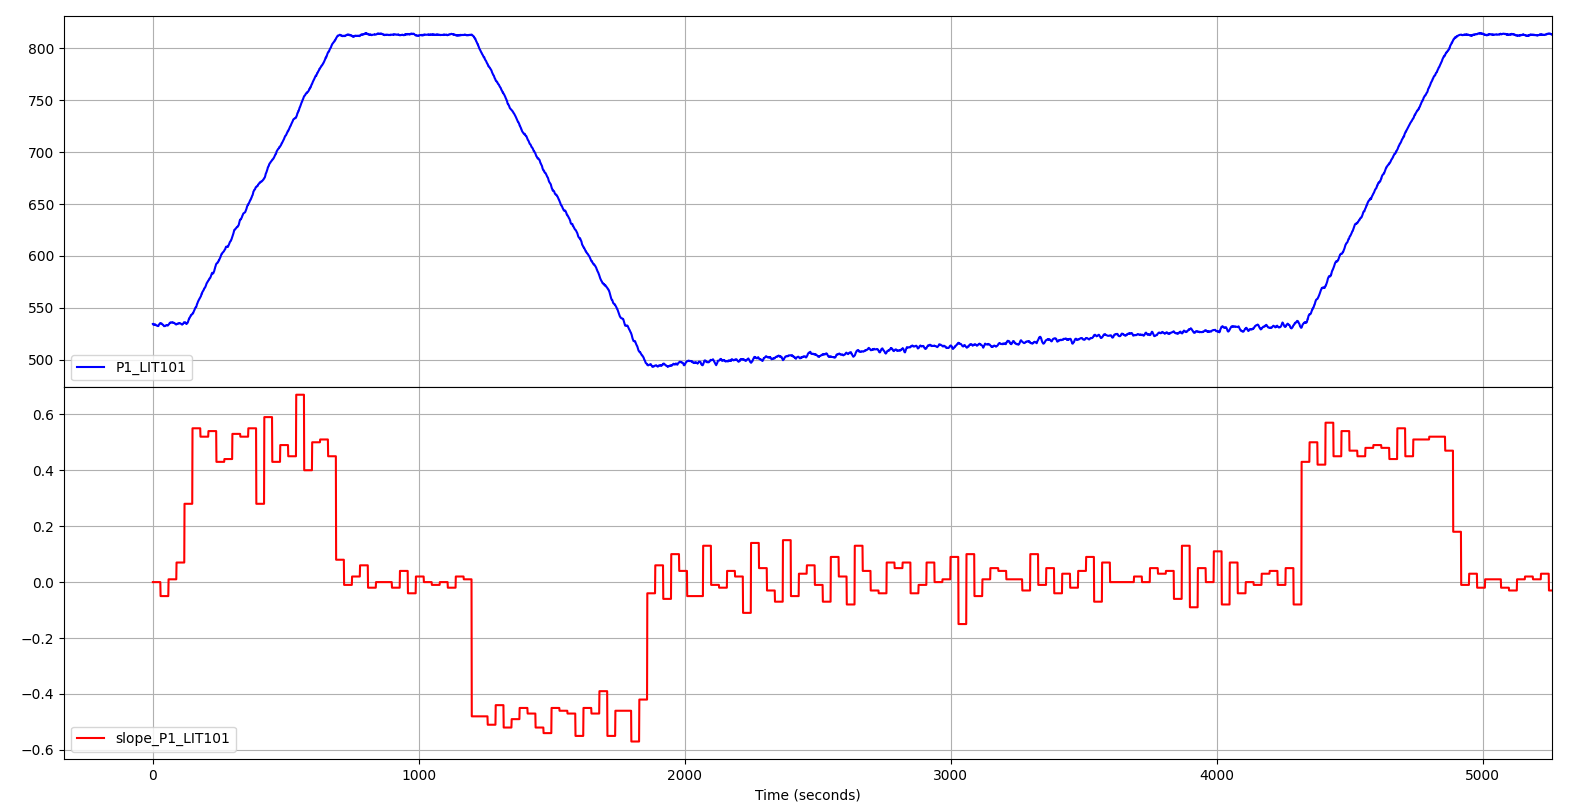
\includegraphics[width=\textwidth]{chap4/slope_nodecomp_g30_2.png}
		\caption{}
		\label{subfig:4_slope_g30_nodecomp}
	\end{subfigure}
	\hfill
	\begin{subfigure}{0.9\textwidth}
		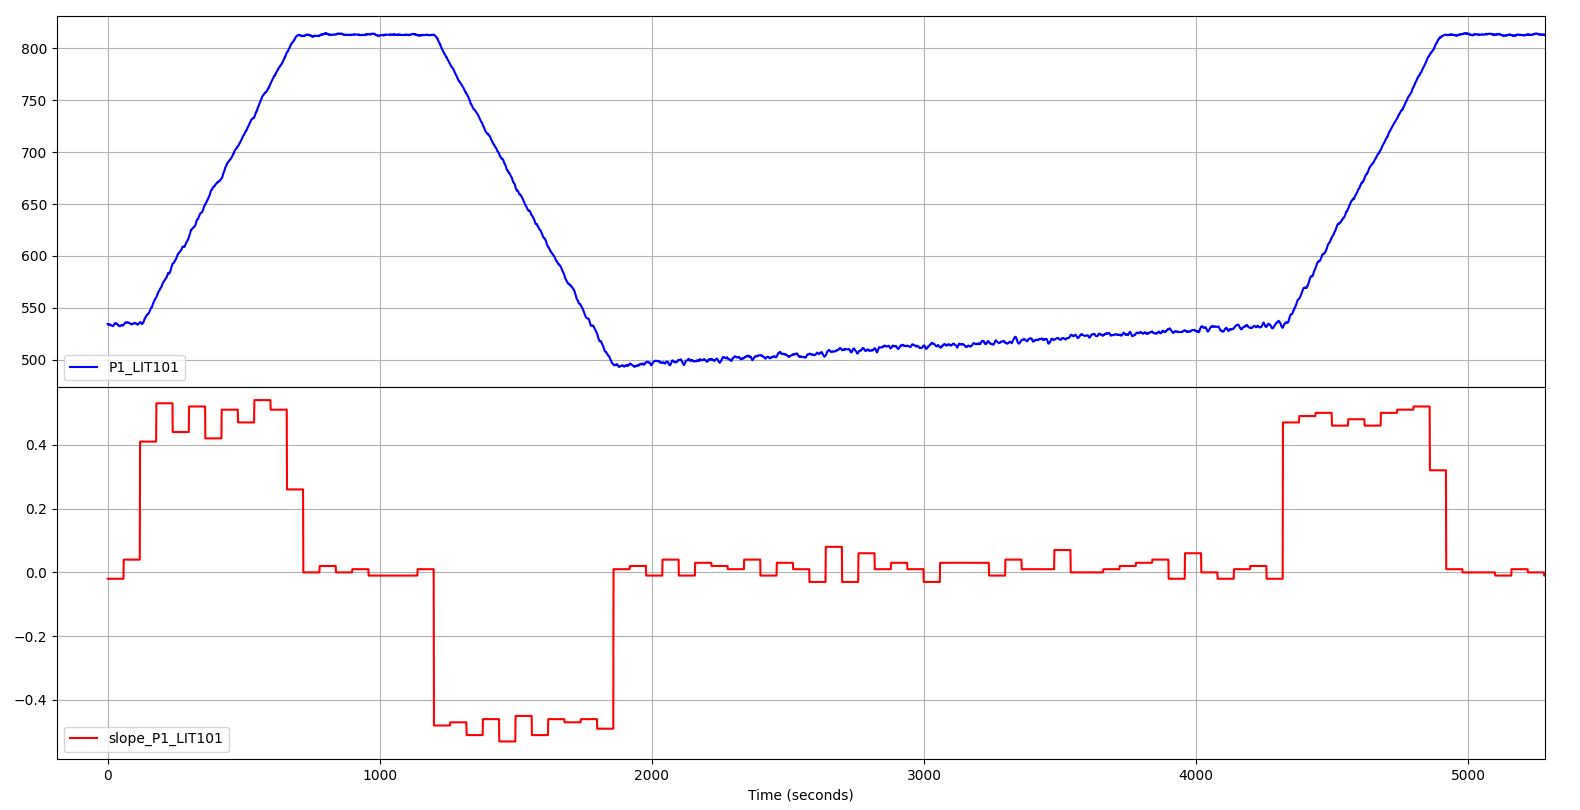
\includegraphics[width=\textwidth]{chap4/slope_nodecomp_g60_2.png}
		\caption{}
		\label{subfig:4_slope_g60_nodecomp}
	\end{subfigure}
	\begin{subfigure}{0.9\textwidth}
		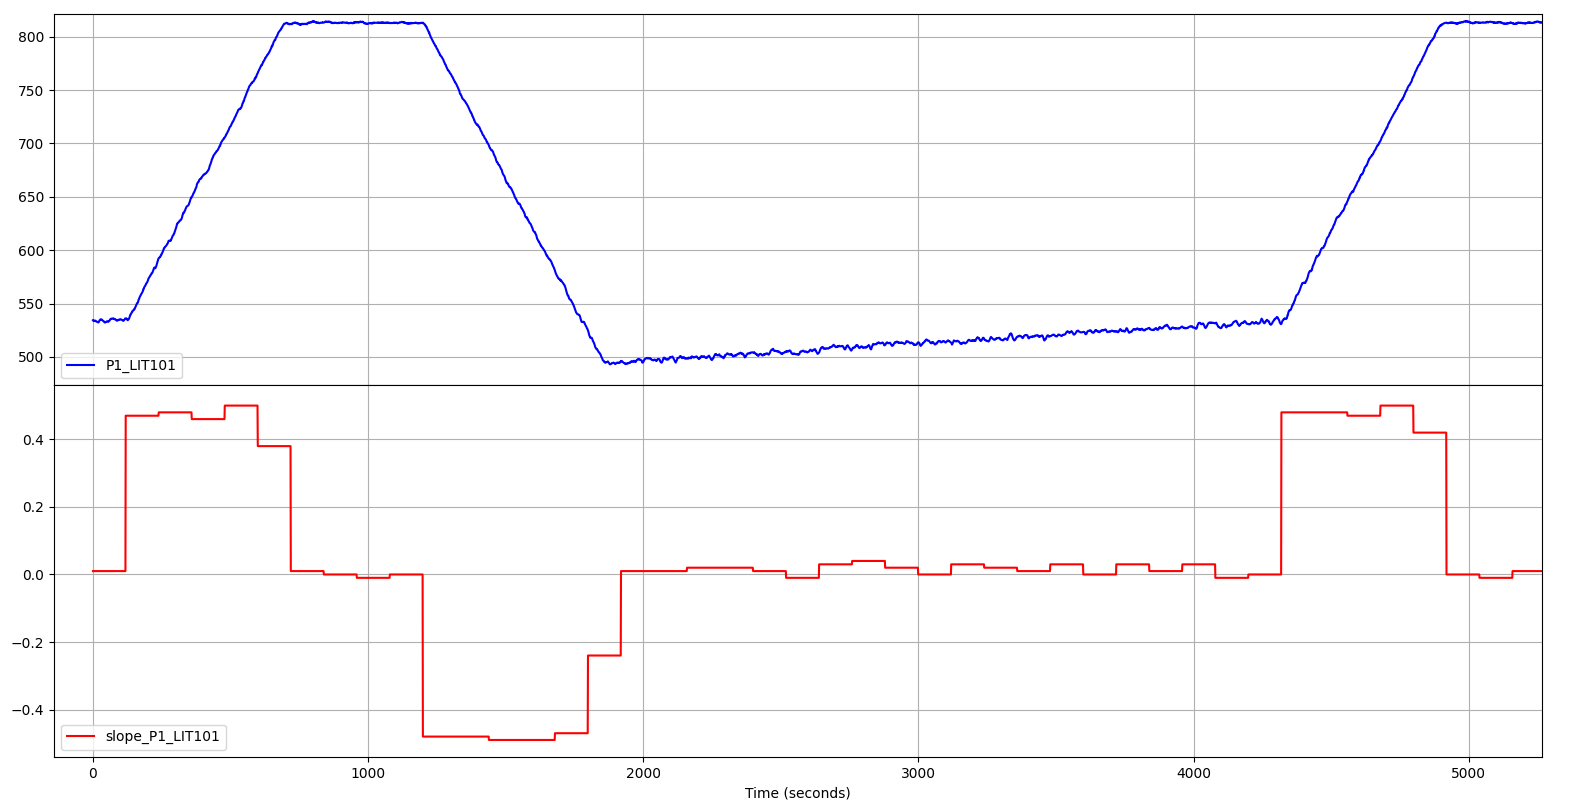
\includegraphics[width=\textwidth]{chap4/slope_nodecomp_g120_2.png}
		\caption{}
		\label{subfig:4_slope_g120_nodecomp}
	\end{subfigure}
	\caption{Slope comparison with granularity 30 (a), 60 (b) and 120 seconds (c)}
	\label{fig:4_slope_comparison}
\end{figure}

The solution to this problem involves applying techniques to reduce the "noise" in the data, aiming to achieve a more linear trend in the measurement curve. By minimizing the effects of perturbations, we can calculate slopes more accurately.\newline
There are various methods available for smoothing out noise in the data. In our framework, we focused on two commonly used approaches found in the literature: \textbf{polynomial regression} and \textbf{seasonal decomposition}. In addition to these two methods, we also explored the use of a \textbf{line simplification algorithm}.\newline \newline
\textit{Polynomial regression} \cite{polynomial_regression} is a technique that allows us to create a filter to reduce the impact of noise on the data. By fitting a polynomial function to the measurements, we can obtain a smoother curve that captures the underlying trend while minimizing the effects of perturbations.\newline
\textit{Seasonal decomposition} \cite{seasonal_decomposition}, specifically the part related to trending, is another method we explored. It involves decomposing the time series into different components, such as trend, seasonality, and residual. By isolating the trend component, we can obtain a cleaner representation of the underlying pattern in the data.\newline
\textit{Line simplification algorithms} \cite{line_simplification_algo} aim to reduce the complexity of a polyline or curve by approximating it with a simplified version composed of fewer points. By selectively removing redundant or less significant points, line simplification algorithms help reduce storage space and computational requirements while preserving the overall shape and characteristics of the original line.\newline
Regarding polynomial regression, we evaluated the use of the \textbf{Savitzky-Golay filter} \cite{savgol} as a smoothing technique. For seasonal decomposition, we explored the \textbf{Seasonal-Trend decomposition using LOESS} (STL) method \cite{stl_decomp}. For the line simplification algorithm, we specifically considered the \textbf{Ramer-Douglas-Peucker} (RDP) algorithm \cite{ramer-douglas-peucker}.\newline \newline
%For lacking of space we are unable to provide a detailed description of the polynomial regression and seasonal decomposition techniques in this context. We recommend referring to the bibliographical notes or relevant literature for a more comprehensive understanding of these methods. 
Figure \ref{fig:4_smoothing_comparison} shows a quick graphical comparison of these techniques compared with the original data. The solution adopted is the \textit{STL decomposition} method, which effectively reduces noise compared to the Savitzky-Golay filter. However, it should be noted that this method may introduce some delay in certain parts of the data, as is typically observed in similar algorithms. Despite its apparent effectiveness, the RDP algorithm fails to accurately approximate sections where the measurement level remains relatively stable. Consequently, it yields incorrect slope estimations, causing a loss of valuable information about the system.

\begin{figure}[H]
	\centering
	\begin{subfigure}{0.48\textwidth}
		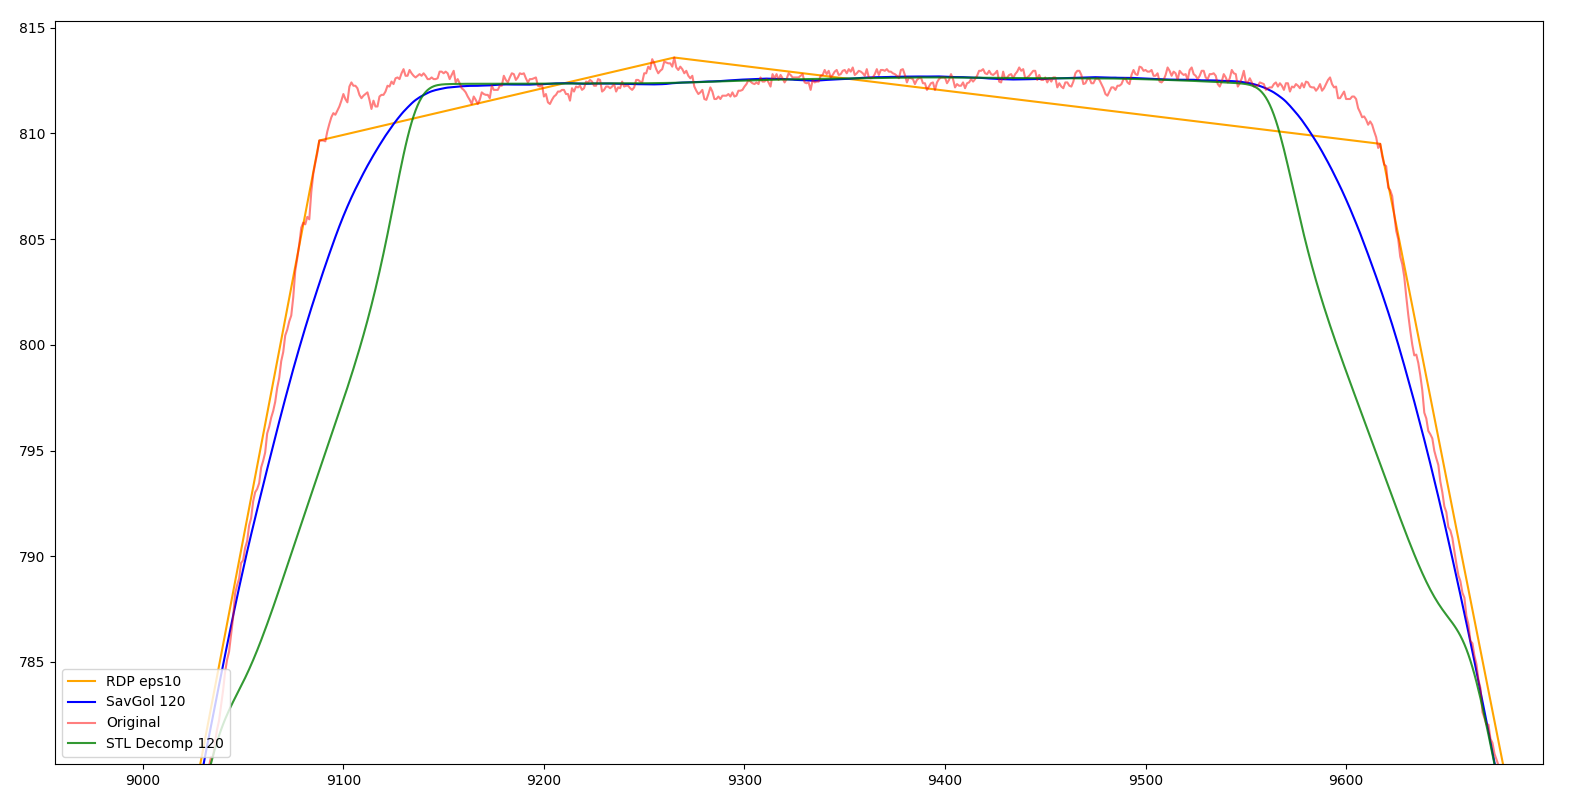
\includegraphics[width=\textwidth]{chap4/confronto_RDP_SavGol_STL_1.png}
		\caption{}
		\label{subfig:4_smoothing1}
	\end{subfigure}
	\hfill
	\begin{subfigure}{0.48\textwidth}
		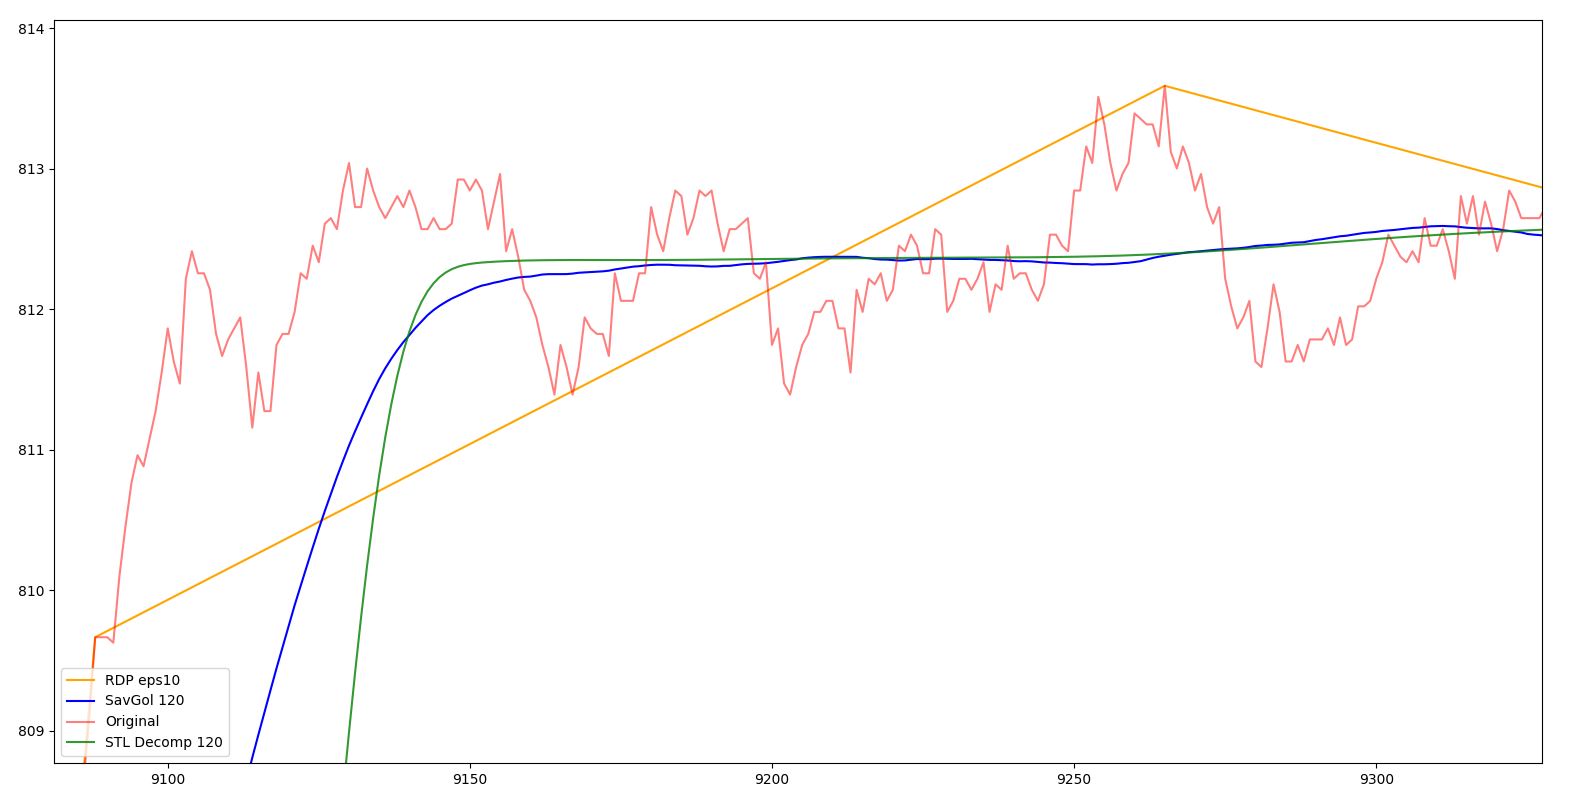
\includegraphics[width=\textwidth]{chap4/confronto_RDP_SavGol_STL_2.png}
		\caption{}
		\label{subfig:4_smoothing2}
	\end{subfigure}
	\begin{subfigure}{0.48\textwidth}
		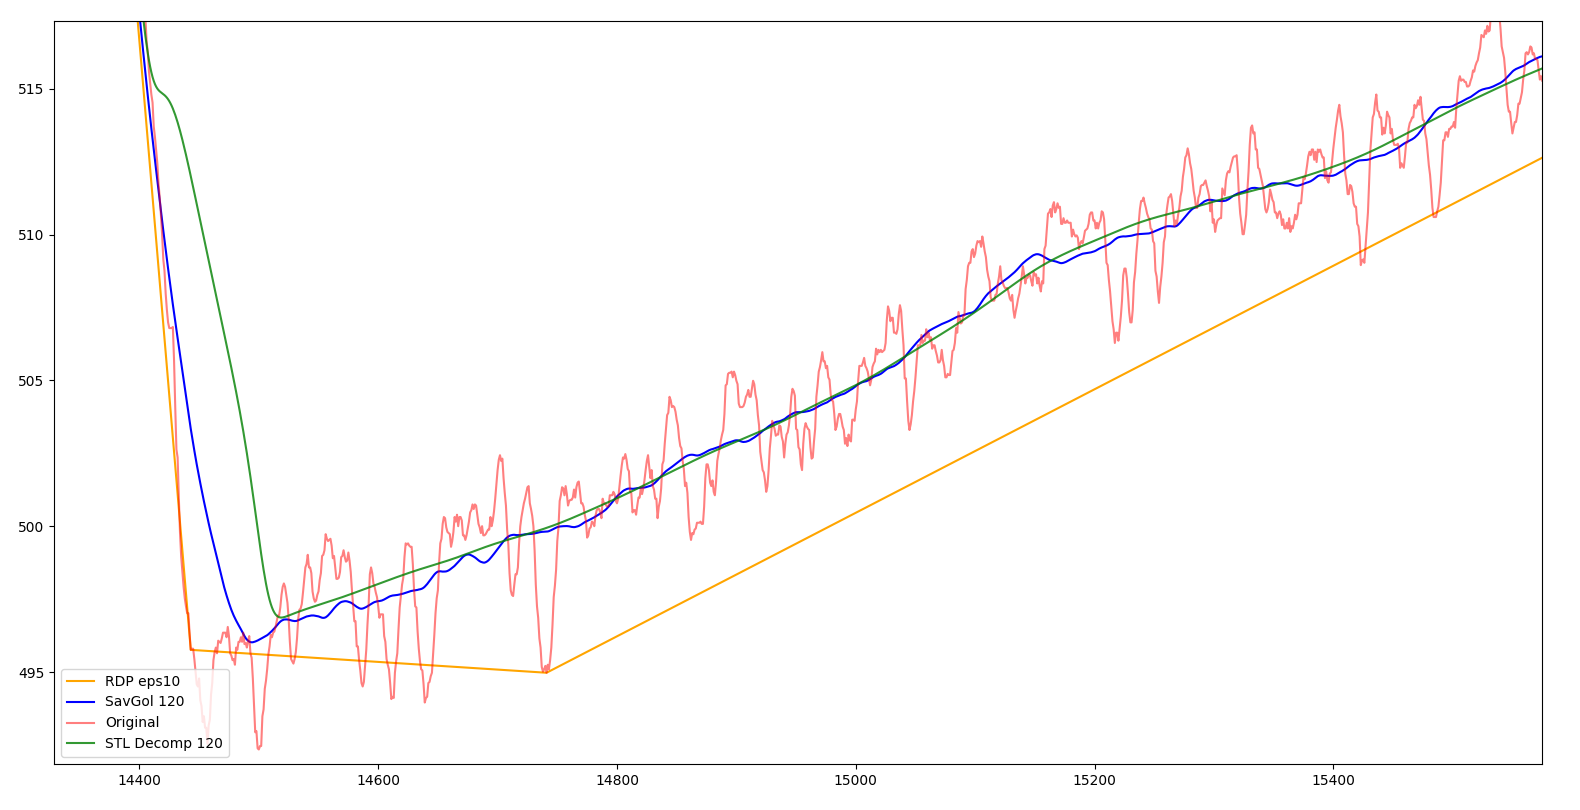
\includegraphics[width=\textwidth]{chap4/confronto_RDP_SavGol_STL_3.png}
		\caption{}
		\label{subfig:4_smoothing3}
	\end{subfigure}
	\hfill
	\begin{subfigure}{0.48\textwidth}
		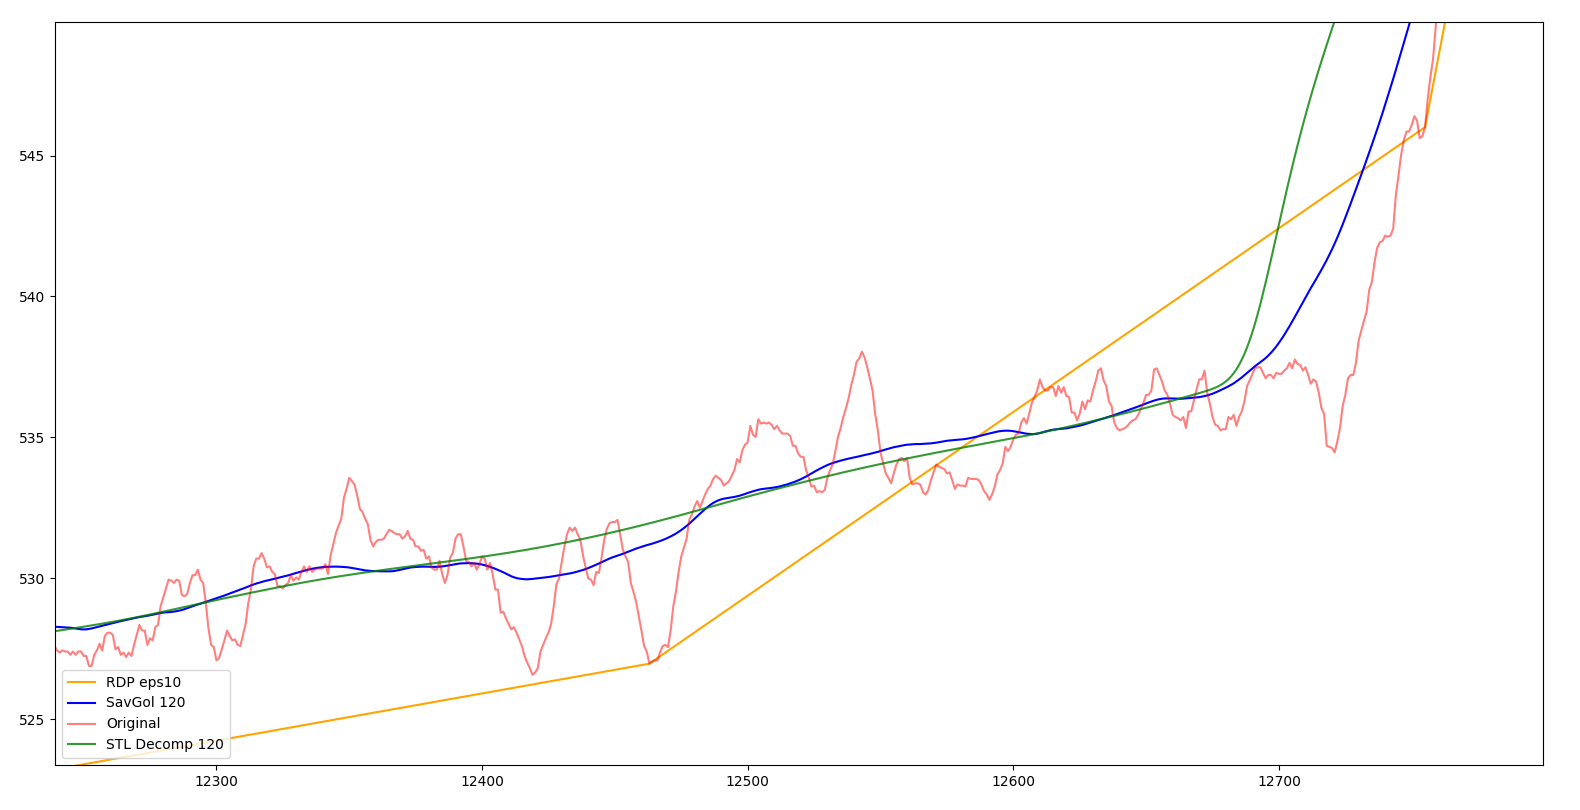
\includegraphics[width=\textwidth]{chap4/confronto_RDP_SavGol_STL_4.png}
		\caption{}
		\label{subfig:4_smoothing4}
	\end{subfigure}
	\caption{Savitzky-Golay filter (blue line), STL decomposition (green) and RDP algorithm (orange) comparison}
	\label{fig:4_smoothing_comparison}
\end{figure}
By applying the STL decomposition, we observe a notable enhancement in slope calculation even when using a low granularity. Figure \ref{fig:4_STL_decomp_results} demonstrates that, with the same granularity as shown in Figure \ref{subfig:4_slope_g30_nodecomp}, the slope values, albeit exhibiting fluctuations, consistently align with the underlying trend of the data curve. The introduced lag resulting from the decomposition's periodicity is responsible for the observed delay.

\begin{figure}[ht]
	\centering
	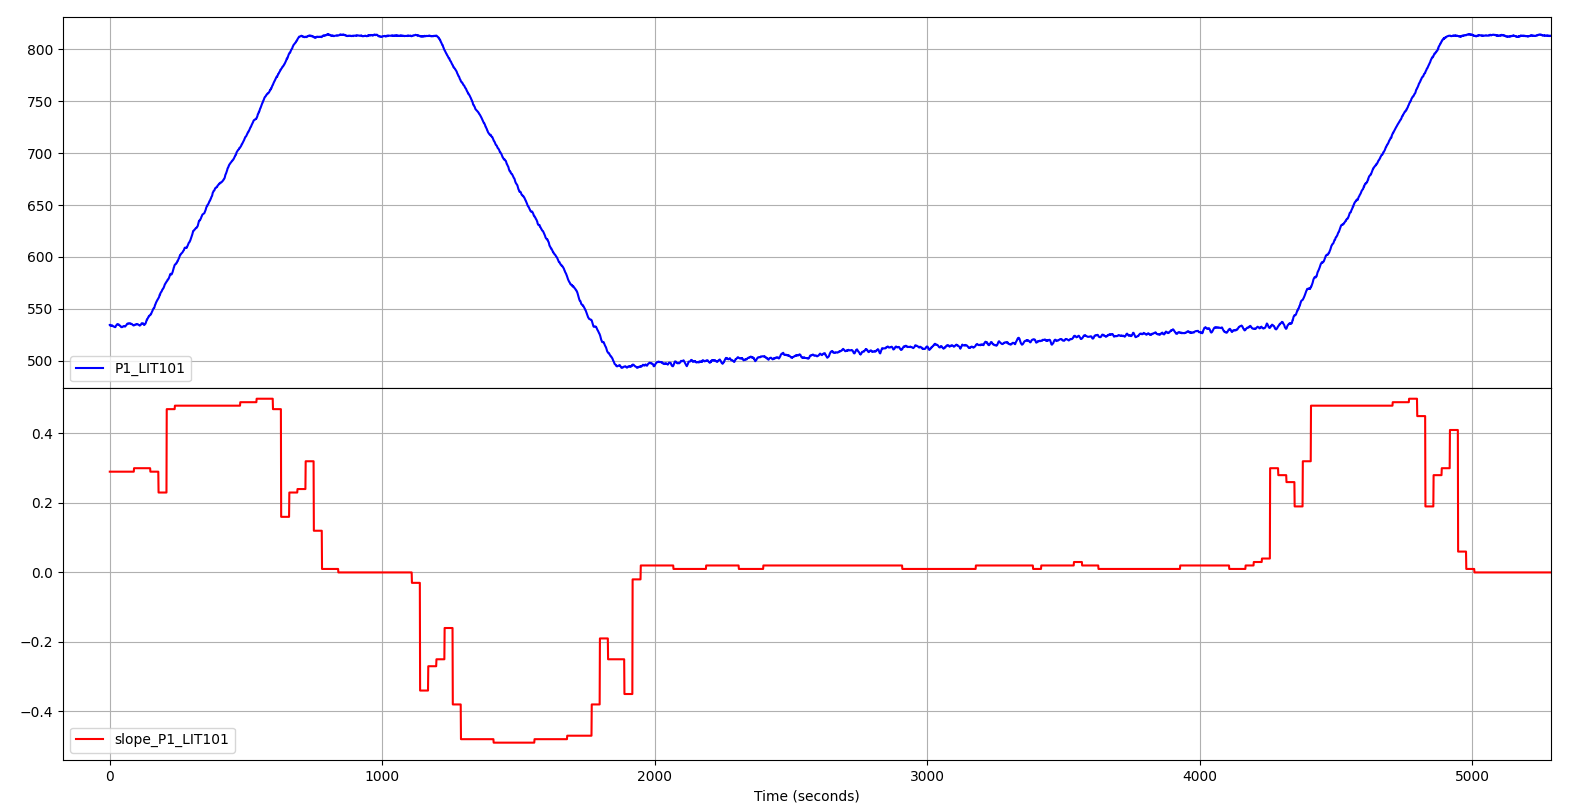
\includegraphics[scale=0.35]{chap4/slope_STL_g30_2.png}
	\caption{Slope after the application of the STL decomposition}
	\label{fig:4_STL_decomp_results}
\end{figure}
The periodicity, which defines the sampling time window for decomposition and the level of noise smoothing, can be configured using the \texttt{trend\_period} directive in the \textit{config.ini} file.\newline
During the slope calculation, the analysis will be performed on the data from the additional measurement trend attributes specified in the \texttt{trend\_cols\_list} directive of the configuration file, rather than on the original unfiltered data.

\bigskip
To ensure proper interpretation by Daikon, the decimal values representing the calculated slopes are converted into \textbf{three numerical values}: -1, 0, and 1. These values correspond to \textit{decreasing} (if the slope is less than zero), \textit{stable} (if it is equal to zero), and \textit{increasing} (if it is greater than zero) trends, respectively. Figure \ref{fig:4_slope_daikon} displays the modified slopes along with the curve obtained from the STL decomposition:

\begin{figure}[ht]
	\centering
	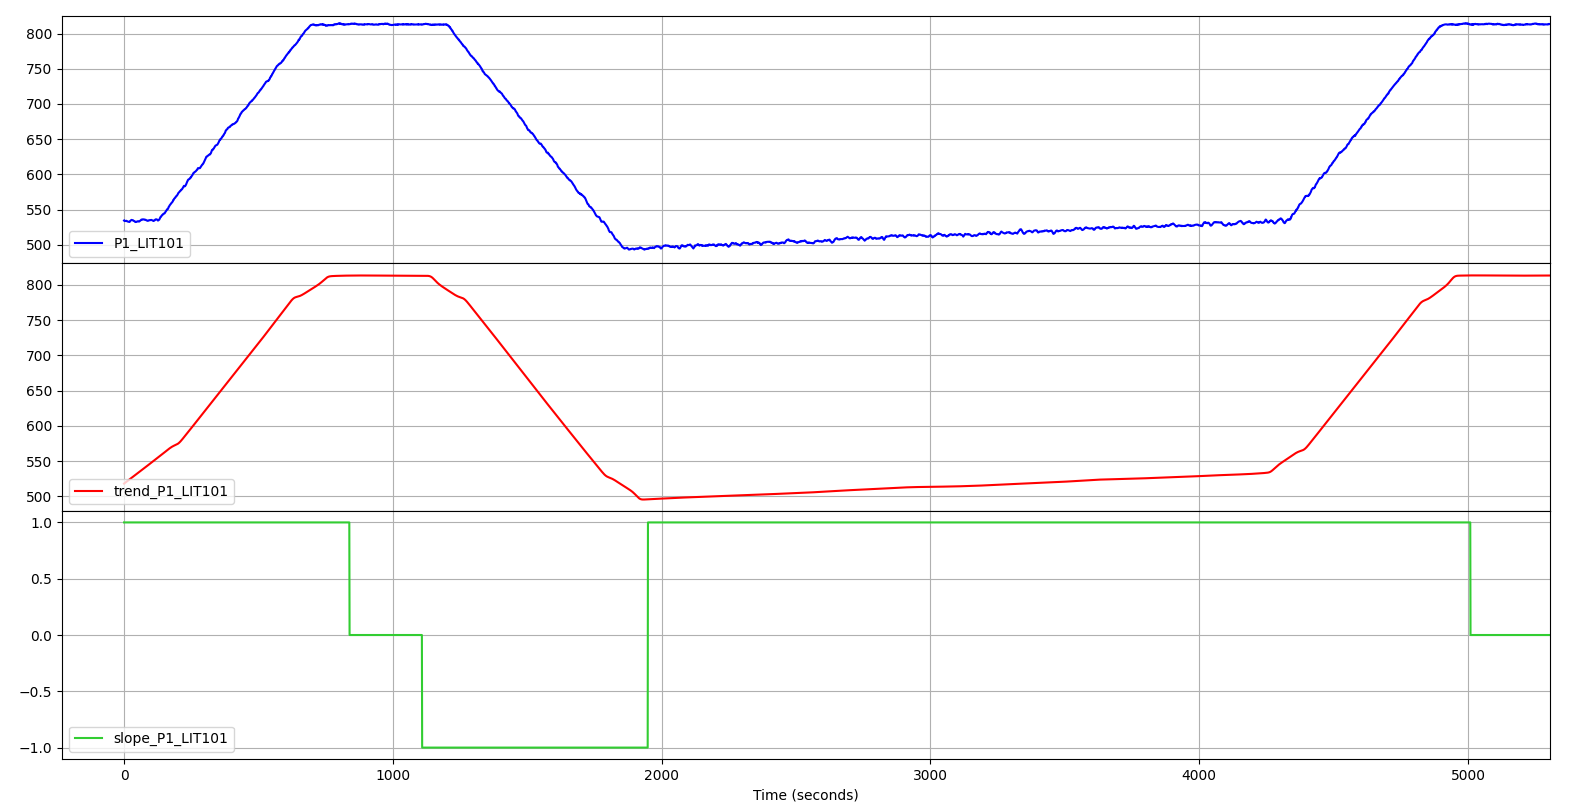
\includegraphics[scale=0.35]{chap4/slope_STL_bin_g30_2b.png}
	\caption{The new slope representation (green line) and the smoothed measurement data obtaind with the STL decomposition (red)}
	\label{fig:4_slope_daikon}
\end{figure}

\subsubsection{Datasets Merging}
\label{subsubsec:4_dataset_merging}
During this step, the datasets of the individual PLCs are merged, resulting in two separate datasets. The first dataset is enriched with additional attributes but excludes the timestamp column. This dataset is intended for inference and invariant analysis. The second dataset does not contain any additional data and is specifically used in the process mining phase.

\bigskip
By default, the enriched dataset will be saved in CSV format in the \texttt{\$(project-dir)/daikon/Daikon\_Invariants} directory. The other dataset, without additional data, will be saved in the \texttt{\$(project-dir)/process-mining/data directory}. It's worth noting that both paths can be configured in the \textit{config.ini} file. The dataset name can be specified in the \textit{config.ini} file or through the \texttt{-o} command-line option. When generating the dataset for process mining, the script will automatically add a \texttt{\_TS} suffix to the filename to indicate that it includes the timestamp. This flexibility allows the user to provide a different filename for each output, preventing overwriting of previous datasets. It enables the user to save the execution trace of the selected subsystem separately and utilize them in subsequent analysis phases.

\subsubsection{Brief Analysis of the Obtained Subsystem}
\label{subsubsec:4_brief_analysis}

After merging the datasets, the user has the option to perform an \textbf{optional analysis} of the resulting dataset to extract preliminary data. This analysis aims to gather basic information about the (sub)system and potentially refine the enrichment process. If the user chooses to proceed with the analysis, the \texttt{mergeDatasets.py} script invokes another Python script located in the \texttt{\$(project-dir)/pre-processing} directory called \texttt{system\_info.py}.\newline
Relying on an analysis based on a combination of Daikon and Pandas this script performs a quick analysis of the dataset allowing to \textbf{estimate}, albeit approximately, the \textbf{type of registers} (sensors, actuators, ...), also identifying possible maximum and minimum values of measurements and hardcoded setpoints. Furthermore, leveraging the use of the additional attribute \texttt{prev\_}, the \texttt{system\_info.py} script is capable of deriving measurement values corresponding to state changes of individual actuators. This allows for the identification of specific measurements associated with the activation or deactivation of certain actuators within the system.\newline
As the last information we have duration of actuator states for each cycle of the system: this information can be useful for making assumptions and conjectures about the behavior of an actuator in a specific state or, by observing the duration values of each cycle, highlighting anomalies in the system. \newline
Listing \ref{lst:4_brief_infos} shows an example of this brief analysis related to PLC1 of the iTrust SWaT system (for brevity, only one measurement is reported in the analysis of actuator state changes):

\begin{lstlisting}[language=bash,numbers=none,caption={Example of preliminar system analysis},label=lst:4_brief_infos]
	Do you want to perform a brief analysis of the dataset? [y/n]: y
	
	Actuators: 
	P1_MV101 [0.0, 1.0, 2.0]
	P1_P101 [1.0, 2.0]
	
	Sensors: 
	P1_FIT101 {'max_lvl': 2.7, 'min_lvl': 0.0}
	P1_LIT101 {'max_lvl': 815.1, 'min_lvl': 489.6}
	
	Hardcoded setpoints or spare actuators: 
	P1_P102 [1.0]
	
	Actuator state changes:
	       P1_LIT101  P1_MV101  prev_P1_MV101
	669     800.7170         0              2
	1850    499.0203         0              1
	4876    800.5992         0              2
	6052    498.9026         0              1
	9071    800.7170         0              2
	10260   499.1381         0              1
	13268   801.3058         0              2
	14435   498.4315         0              1
	17423   801.4628         0              2
	18603   498.1567         0              1
	
	P1_LIT101  P1_MV101  prev_P1_MV101
	677     805.0741         1              0
	4885    805.7414         1              0
	9079    805.7806         1              0
	13276   805.1133         1              0
	17432   804.4068         1              0
	
	P1_LIT101  P1_MV101  prev_P1_MV101
	1858    495.4483         2              0
	6060    497.9998         2              0
	10269   495.9586         2              0
	14443   495.8016         2              0
	18611   494.5847         2              0
	
	       P1_LIT101  P1_P101  prev_P1_P101
	118     536.0356        1             2
	4322    533.3272        1             2
	8537    542.1591        1             2
	12721   534.8581        1             2
	16883   540.5890        1             2
	
	P1_LIT101  P1_P101  prev_P1_P101
	1190    813.0031        2             1
	5395    813.0031        2             1
	9597    811.8256        2             1
	13776   812.7283        2             1
	17938   813.3171        2             1
	
	Actuator state durations:
	P1_MV101 == 0.0
	9  9  10  9  9  10  9  9  10  9
	
	P1_MV101 == 1.0
	1174  1168  1182  1160  1172
	
	P1_MV101 == 2.0
	669  3019  3012  3000  2981
	
	P1_P101 == 1.0
	1073  1074  1061  1056  1056
	
	P1_P101 == 2.0
	118  3133  3143  3125  3108
\end{lstlisting}

From these results we can draw the following conjectures: 

\begin{itemize}
	\item the \textbf{probable actuators} are \texttt{P1\_MV101} and \texttt{P1\_P101}. \texttt{P1\_MV101} has three states identified by the values 0, 1, and 2, suggesting it is a multi-state actuator. \texttt{P1\_P101} has two states identified by the values 1 and 2, indicating a binary actuator;
	
	\item there are \textbf{two probable measures}: \texttt{P1\_FIT101} and \texttt{P1\_LIT101}. \texttt{P1\_FIT101} has values ranging from 0 to 2.7, \texttt{P1\_LIT101} has values ranging from 489.6 to 815.1. Based on this information, a further conjecture can be made that \texttt{P1\_LIT101} represents a tank level measurement;
		
	\item apparently there is a probable \textbf{spare actuator}, \texttt{P1\_P102}, whose value is always 1. No related \textit{hardcoded setpoints} were found. From this information, another speculation can be made that the value 1 represents the \textbf{OFF state} for binary actuators, while the value 2 represents the \textbf{ON state};
	
	\item from the analysis of state changes we can derive some \textbf{relative setpoints}. For example, we observe that \texttt{P1\_P101} changes state from value 1 (OFF) to value 2 (ON) when the level of \texttt{P1\_LIT101} is approximately 813, and it changes from value 2 (ON) to 1 (OFF) when the level of \texttt{P1\_LIT101} is around 535. We can deduce that \texttt{P1\_P101} is responsible for emptying the tank;
	
	\item Regarding the actuators states duration, the very short duration of \texttt{P1\_MV101} in state 0 is observable: since we are unable, at this preliminary stage, to make assumptions about this, we will try to understand the behavior of the system in this actuator state in the next stages of the analysis.
\end{itemize}

The information obtained here can be used, as mentioned above, to refine the enrichment of the dataset by setting directives in the \texttt{[DATASET]} section of the \textit{config.ini} file, should this be empty or only partially set, or to make the first conjectures about the system, as we have just seen.

\bigskip
The \texttt{system\_info.py} file can also run in standalone mode if needed: it takes as command-line arguments the dataset to be analyzed, a list of actuators, and a list of sensors. For analysis related to state changes, the dataset must mandatorily be of the enriched type.

\subsection{Phase 2: Graphs and Statistical Analysis}
\label{subsec:4_improve_graphs}

The new \textit{graph analysis} arises from the need to give the user an overview of the (sub)system obtained in the previous pre-processing phase, identifying more easily the typology of the registers and grasping more effectively the relationships and the dynamics that may exist between the registers controlled by one or more PLCs, confirming the initial conjectures if the brief analysis described in the previous section has been performed, or making new ones thanks to the visual graph support. 

\bigskip
In Ceccato et al.'s framework, as mentioned in Section \ref{subsec:3_ceccato_limitations}, it was only possible to view the chart of one register at a time. While this allowed for the identification or hypothesis of the register type, it made it challenging to establish relationships with other components of the system and derive conjectures about their behavior. To address this limitation, there was a need for a new tool that could provide more information in a more accessible manner.

\bigskip
Initially, we considered adopting an approach similar to Figure \ref{fig:graph_analysis_prop3}, where all the graphs are displayed within a single plot. However, we soon realized that this solution was not feasible and could not be adopted. Figure \ref{fig:4_plot_comparison_1} helps to understand why.  

\begin{figure}[H]
	\centering
	\begin{subfigure}{0.48\textwidth}
		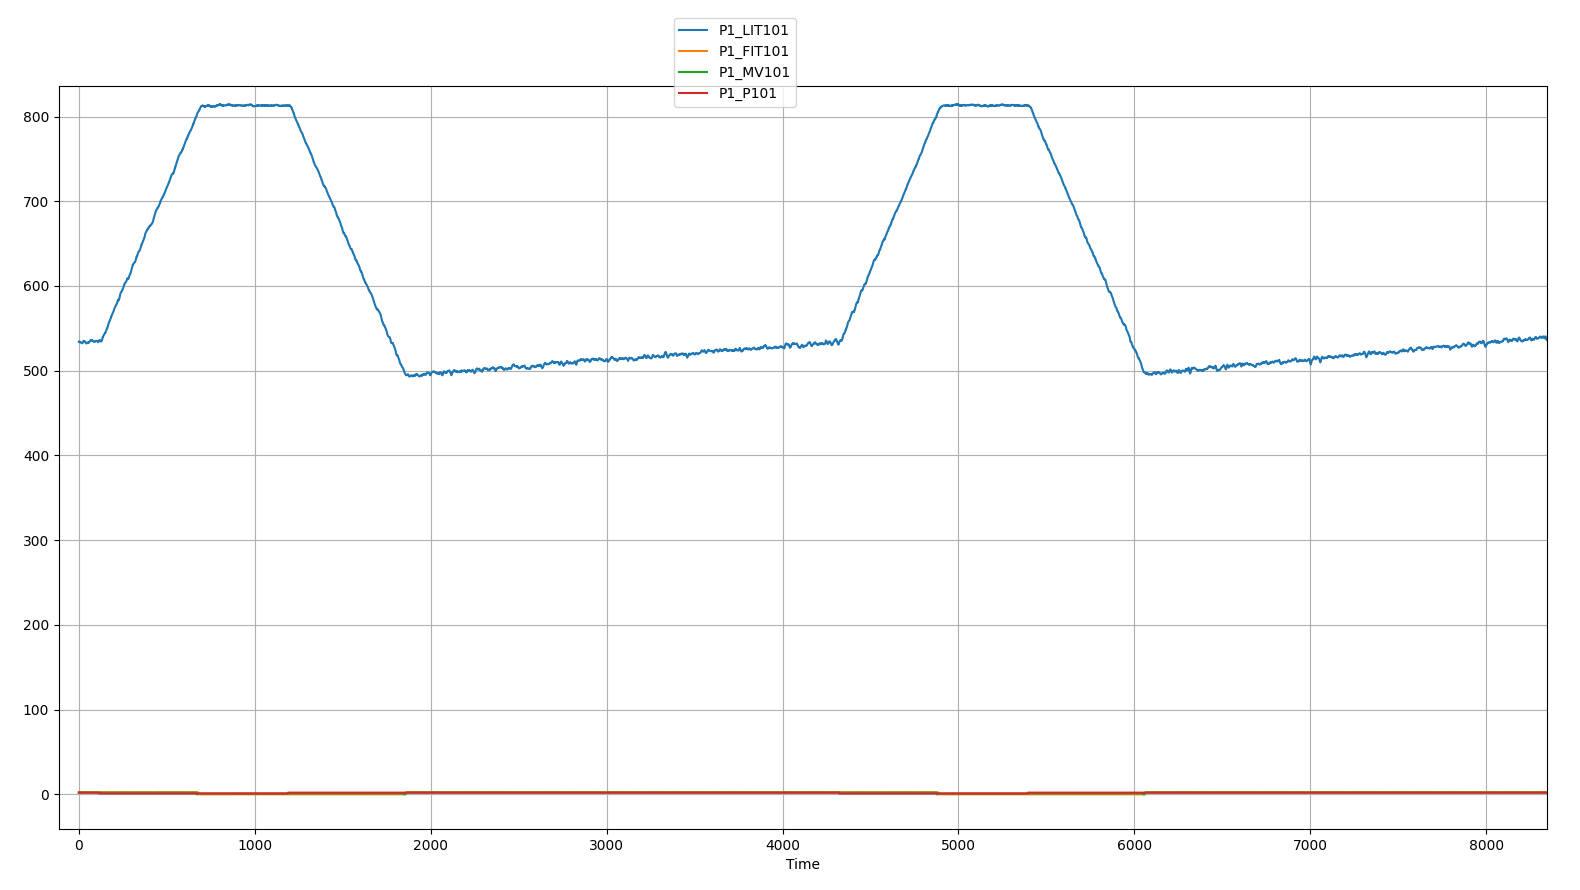
\includegraphics[width=\textwidth]{chap4/wrong_plot_1.png}
		\caption{}
		\label{subfig:4_wrong_plot}
	\end{subfigure}
	\hfill
	\begin{subfigure}{0.48\textwidth}
		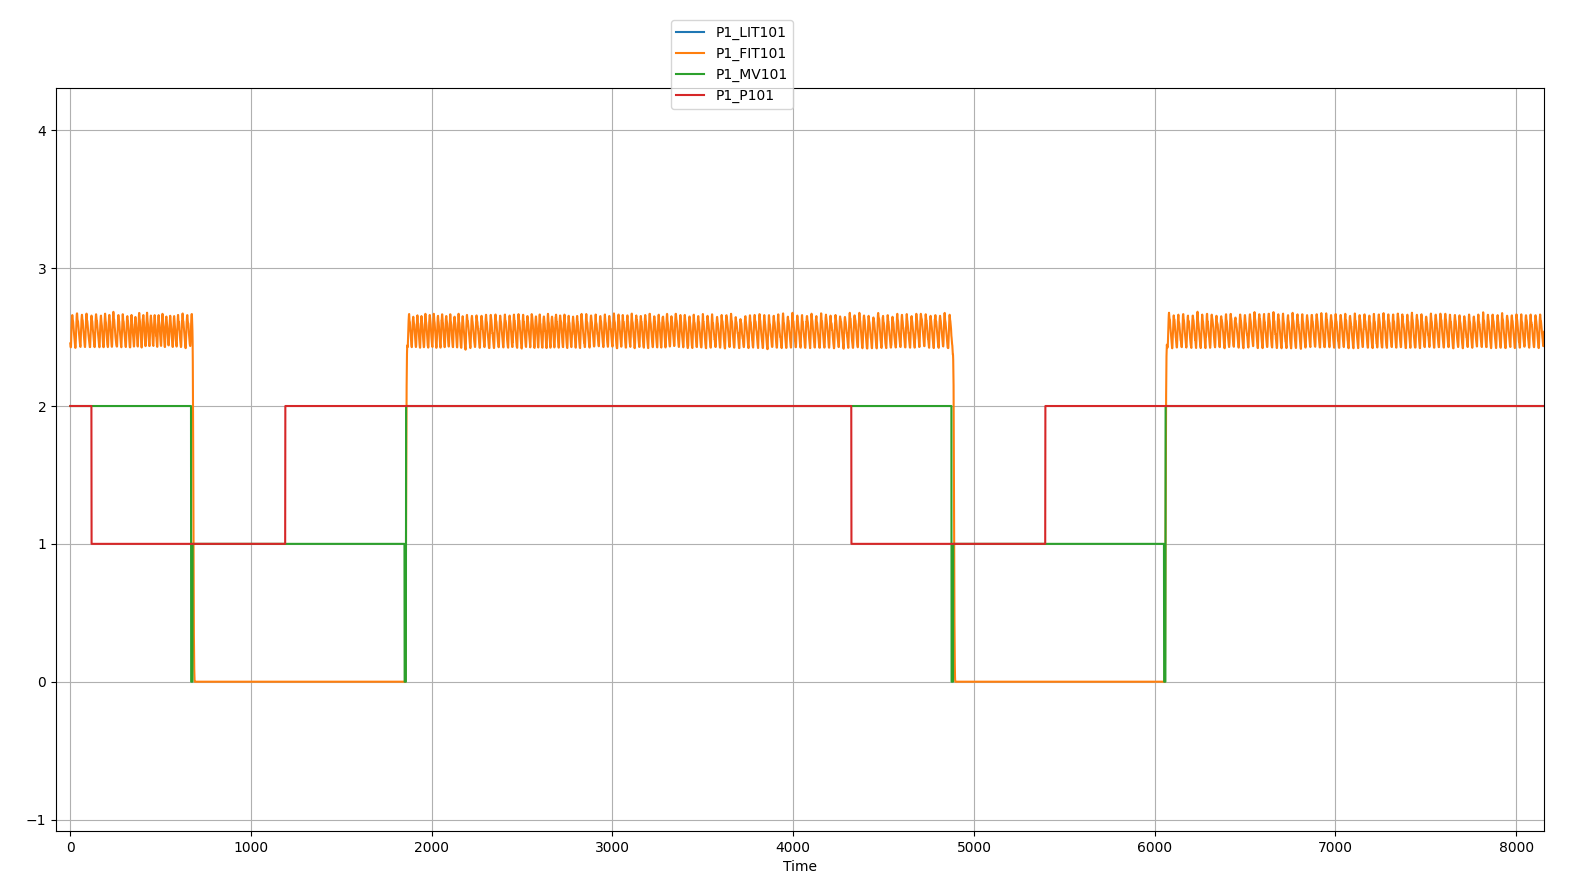
\includegraphics[width=\textwidth]{chap4/wrong_plot_2.png}
		\caption{}
		\label{subfig:4_wrong_plot_zoom}
	\end{subfigure}
	\caption{Plotting registers on the same y-axis}
	\label{fig:4_plot_comparison_1}
\end{figure}
Figure \ref{subfig:4_wrong_plot} highlights the main issue with this approach, which is the use of the same y-axis for all the charts, representing the values of individual registers. When the range between register values is wide, it can result in some charts appearing as a single flat line or becoming indistinguishable, making them difficult to read. Additionally, as shown in Figure \ref{subfig:4_wrong_plot_zoom}, when registers have similar values, the graphs can become confusing and harder to interpret.

\bigskip
The solution to this issue is simple and effective: the use of \textbf{subplots}. Basically, each register corresponds to a subplot of the graph that shares the time axis (the x-axis) with the other subplots, but keeps the y-axis of the values of each register independent. This maintains the readability and comprehensibility of the charts, while simultaneously being able to immediately grasp the relationships between them. In addition, by sharing the time axis, it is possible to zoom in on a particular area of one of the charts and automatically the other ones will be zoomed in as well, thus not losing any information and no connection between registers. Figure \ref{fig:4_graph_analysis} illustrates more clearly what has just been explained: the charts refer to the PLC1 registers of the iTrust SWaT system.

\begin{figure}[H]
	\centering
	\begin{subfigure}{0.9\textwidth}
		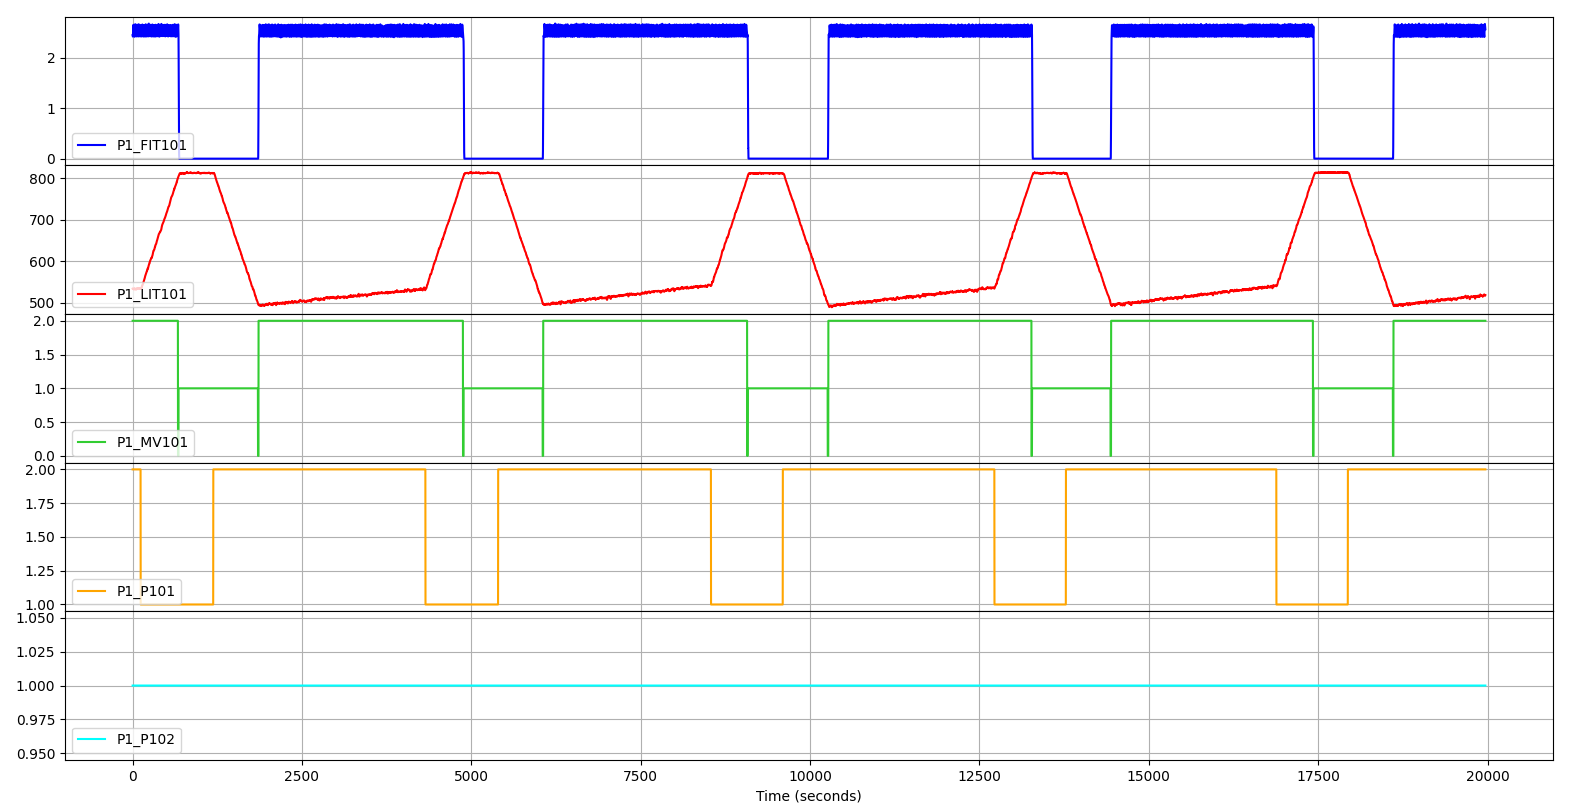
\includegraphics[width=\textwidth]{chap4/graph_analysis_plot_1.png}
		\caption{Example of plotting charts of a PLC registers using subplots}
		\label{subfig:4_graph_analysis_1}
	\end{subfigure}
	\hfill
	\begin{subfigure}{0.9\textwidth}
		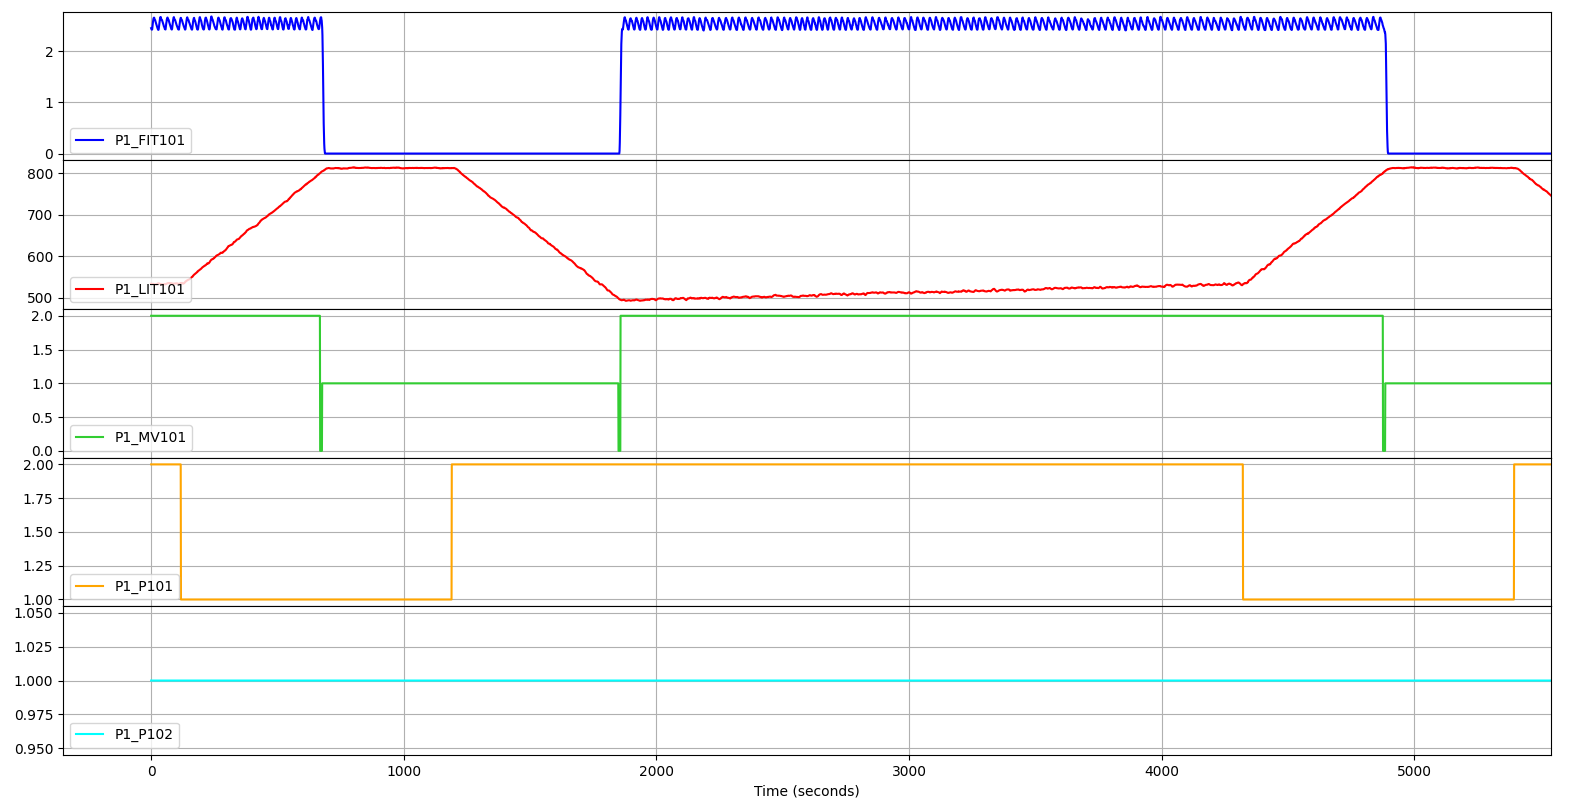
\includegraphics[width=\textwidth]{chap4/graph_analysis_plot_2.png}
		\caption{Zooming on a particular zone of the charts}
		\label{subfig:4_graph_analysis_2}
	\end{subfigure}
	\caption{Example of the new graph analysis}
	\label{fig:4_graph_analysis}
\end{figure}

\bigskip
To demonstrate the behavior and effectiveness of the new graph analysis process, we observe in particular, Figure \ref{subfig:4_graph_analysis_2}: we can already have some validation on the conjectures made in the brief analysis from the previous step:

\begin{itemize}
	\item the chart of \texttt{P1\_FIT101} seems to confirm that this register can be associated with a \textbf{measurement}; moreover, we can see that the trend of this register is closely related to the periods in which \texttt{P1\_LIT101} has an increasing trend and to the evolution of \texttt{P1\_MV101}. Its values, between about 0 and 2.5, are too narrow to say that this register represents the tank, and the general trend also leads in that direction: we can therefore assume that it is a \textbf{pressure or flow sensor};
	
	\item \texttt{P1\_LIT101}, because of the above, would therefore seem to \textbf{represent a tank}, as already assumed in the brief analysis;
	
	\item \texttt{P1\_MV101} assumes value 2 at the beginning of the ascending trend of \texttt{P1\_LIT101}, while it has value 1 in correspondence with the \textit{plateau} that is seen when the measurement is about 800 and when the trend of it is descending. Thus, we can have a confirmation of the initial conjecture: 1 represents the OFF state of the sensor, 2 the ON state, and \texttt{P1\_MV101} is the \textbf{actuator responsible for the rising level} of \texttt{P1\_LIT101};
	
	\item \texttt in the brief analysis we observed the short duration of \texttt{P1\_MV101} in state 0, but we were not able to speculate on the reason for this. Graph analysis shows that {P1\_MV101} switches and stays in the 0 state acting as a kind of "transient" between states 1 and 2. It can be assumed that that is the period of time it actually takes for the actuator to change state;
	
	\item \texttt{P1\_P101} assumes value 2 at the beginning of the descending trend of \texttt{P1\_LIT101}, after the \textit{plateu}, and returns to value 1 at the change of slope of the (likely) tank increase: taken by itself this fact is not very clear, so it needs to be compared with \texttt{P1\_LIT101} and \texttt{P1\_MV101} to understand its behavior: it can be seen that when \texttt{P1\_101} and \texttt{P1\_MV101} are in state 1 the water level remains stable, whereas, when \texttt{P1\_P101} changes to state 2 the level of the measurement drops rapidly; when \texttt{P1\_MV101} then also returns to state 2, the level of the measurement slowly starts rising again and then has a sudden rise at the change of state of \texttt{P1\_P101} from 2 to 1. We can therefore infer that \texttt{P1\_P101} is the \textbf{actuator responsible for emptying} the (presumed) tank: state 1 represents the OFF state, while state 2 represents the ON state;
	
	\item \texttt{P1\_P102} seems to play no role in the system, since its state remains at 1 all the time. It seems improbable that it could be a relative setpoint, so it can be assumed, according to the brief analysis, that it may be a \textbf{spare actuator}.
\end{itemize}

\bigskip
As the reader has probably already noticed, The majority of the graphs presented in the previous sections and chapters were generated using the new graph analysis script, specifically the \texttt{runChartsSubPlots.py} script. This Python script is located in the \texttt{\$(project-dir)/statistical-graphs} directory and utilizes the \textit{matplotlib} libraries to generate the graph plots, similar to the previous tool.\newline 
The script accepts the following command-line parameters:

\begin{itemize}
	\item \textbf{-f} or \textbf{{-}{-}filename}: specifies the dataset, in CSV format, from which to read the data. The dataset must be located within the directory containing the enriched datasets for the invariant analysis phase. If subsequent parameters are not specified, the script will show all registers in the dataset, except for additional attributes
	
	\item \textbf{-r} or \textbf{{-}{-}registers}: specifies one or more specific registers to be displayed
	
	\item \textbf{-a} or \textbf{{-}{-}addregisters}: adds one or more registers to the default visualization. This option is useful in case an additional attribute such as slope is to be analyzed
	
	\item \textbf{-e} or \textbf{{-}{-}excluderegisters}: excludes one or more specific registers from the default visualization. This option is useful to avoid displaying hardcoded setpoints or spare registers
\end{itemize}
This script, like the previous ones, is designed to provide the maximum flexibility and ease of use for the user, combined with greater power and effectiveness in deriving useful information about the analyzed system.

\paragraph{Statistical Analysis} After careful consideration, we made the decision not to include the statistical analysis aspect of the previous tool in the framework. We found that there was no practical use for it. Instead, we integrated the relevant statistical information into the brief analysis conducted after the pre-processing phase. Additionally, we deemed the histogram to have limited utility and considered it outdated in comparison to the new graph analysis approach we implemented. \newline
Although we decided not to include the statistical analysis aspect in the framework, the Python script \texttt{histPlots\_Stats.py} from the original tool remains in the directory. This script is essentially unchanged from the version developed by Ceccato et al. and can be used in the future if the need arises. 

\subsection{Phase 3: Invariant Inference and Analysis}
\label{subsec:4_improve_invariants}
The phase of invariant inference and analysis has undergone a redesign and improvement to offer the user a more comprehensive and effortless approach to identify invariants. This has been achieved through the application of new criteria to analyze and reorganize the Daikon analysis results. The outcome of this is a more compact presentation of information that highlights the possible relationships among invariants.\newline
The new design not only enables the identification of undiscovered aspects of the system behavior but also confirms the hypotheses made during the earlier stages of analysis. This step is now semi-automated, unlike before, and allows for the analysis of invariants on individual actuator states and their combinations.

\subsubsection{Revised Daikon Output}
\label{subsub:4_new_daikon_output}
To streamline the process of identifying invariants quickly and efficiently, it is necessary to revise the output generated by standard Daikon analysis. The goal is to create a more compact and readable format for the output.
\newline \newline
The current Daikon results consist of three sections:

\begin{enumerate}
	\item the first section containing generic invariants, i.e., valid regardless of whether a condition is specified for the analysis
	
	\item the second section containing invariants obtained by specifying a condition for the analysis in the \textit{.spinfo} file 
	
	\item a third section containing the invariants that are obtained from the negations of the condition possibly specified in the .spinfo file
\end{enumerate}

In each section only a single invariant per row is shown, without relating it in any way to the others: this makes it difficult to identify significant invariants and any invariant chains that might provide much more information about the behavior of the system than the single invariant.\newline
A brief example of the structure and format of this output related to \texttt{PLC1} of the iTrust SWaT system is shown in Listing \ref{lst:4_daikon_output_plc1}, where a condition was specified on the measurement \texttt{P1\_LIT101} and on actuator \texttt{P1\_MV101}: % sono 61 righe effettive di invarianti - 48 generiche, 10 condizionali, 1 negata

\begin{lstlisting}[language=bash,numbers=none,caption={Standard Daikon output for \texttt{PLC1} of the iTrust SWaT system},label=lst:4_daikon_output_plc1]
	aprogram.point:::POINT
	P1_P102 == prev_P1_P102
	P1_FIT101 >= 0.0
	P1_MV101 one of { 0.0, 1.0, 2.0 }
	P1_P101 one of { 1.0, 2.0 }
	P1_P102 == 1.0
	max_P1_LIT101 == 816.0
	min_P1_LIT101 == 489.0
	slope_P1_LIT101 one of { -1.0, 0.0, 1.0 }
	[...]
	P1_LIT101 > P1_MV101
	P1_LIT101 > P1_P101
	P1_LIT101 > P1_P102
	P1_LIT101 < max_P1_LIT101
	P1_LIT101 > min_P1_LIT101
	[...]
	P1_MV101 < min_P1_LIT101
	P1_MV101 < trend_P1_LIT101
	P1_P101 >= P1_P102
	P1_P101 < max_P1_LIT101
	[...]
  ===============================================
	aprogram.point:::POINT;condition="P1_MV101 == 2.0 && P1_LIT101 < max_P1_LIT101 - 16 && P1_LIT101 > min_P1_LIT101 + 15"
	P1_MV101 == prev_P1_MV101
	P1_P102 == slope_P1_LIT101
	P1_MV101 == 2.0
	P1_FIT101 > P1_MV101
	P1_FIT101 > P1_P101
	P1_FIT101 > P1_P102
	P1_FIT101 > prev_P1_P101
	P1_MV101 >= P1_P101
	P1_MV101 >= prev_P1_P101
	P1_P101 <= prev_P1_P101
  ===============================================
	aprogram.point:::POINT;condition="not(P1_MV101 == 2.0 && P1_LIT101 < max_P1_LIT101 - 16 && P1_LIT101 > min_P1_LIT101 + 15)"
	P1_P101 >= prev_P1_P101
	Exiting Daikon.
\end{lstlisting}

In the presented framework, the output is simplified to \textbf{two sections}: the \textit{general section} and the section related to the \textit{user-specified condition}. The section related to the negated condition is eliminated as it is not relevant in this context and could lead to potential misinterpretation. Moreover, the relationships between invariants will be emphasized by utilizing \textbf{transitive closures}: transitive closure of a relation $R$ is another relation, typically denoted $R^{+}$ that adds to $R$ all those elements that, while not necessarily related directly to each other, can be reached by a \textit{chain} of elements related to each other. In other words, the transitive closure of $R$ is the smallest (in set theory sense) transitive relation $R$ such that $R$ $\subset$ $R^{+}$ \cite{transitive_closures}. 

\bigskip
To implement the transitive closure of the invariants generated by Daikon, we initially categorized the invariants in each section by type based on their equivalence relation, excluding any invariants related to additional attributes except for the slope. For each type of invariant, we constructed a \textbf{graph} using the NetworkX library, where registers were represented as nodes, and arcs were created to connect registers that shared a common endpoint in the invariant, applying the transitive property. To reconstruct the individual invariant chains, then, we used a simple \textit{Depth-first Search} (DFS) on each of the graphs, thus obtaining the desired outcome. Figure \ref{fig:4_transitive_closure_graphs} shows some examples of these graphs:

\begin{figure}[H]
	\centering
	\begin{subfigure}{0.48\textwidth}
		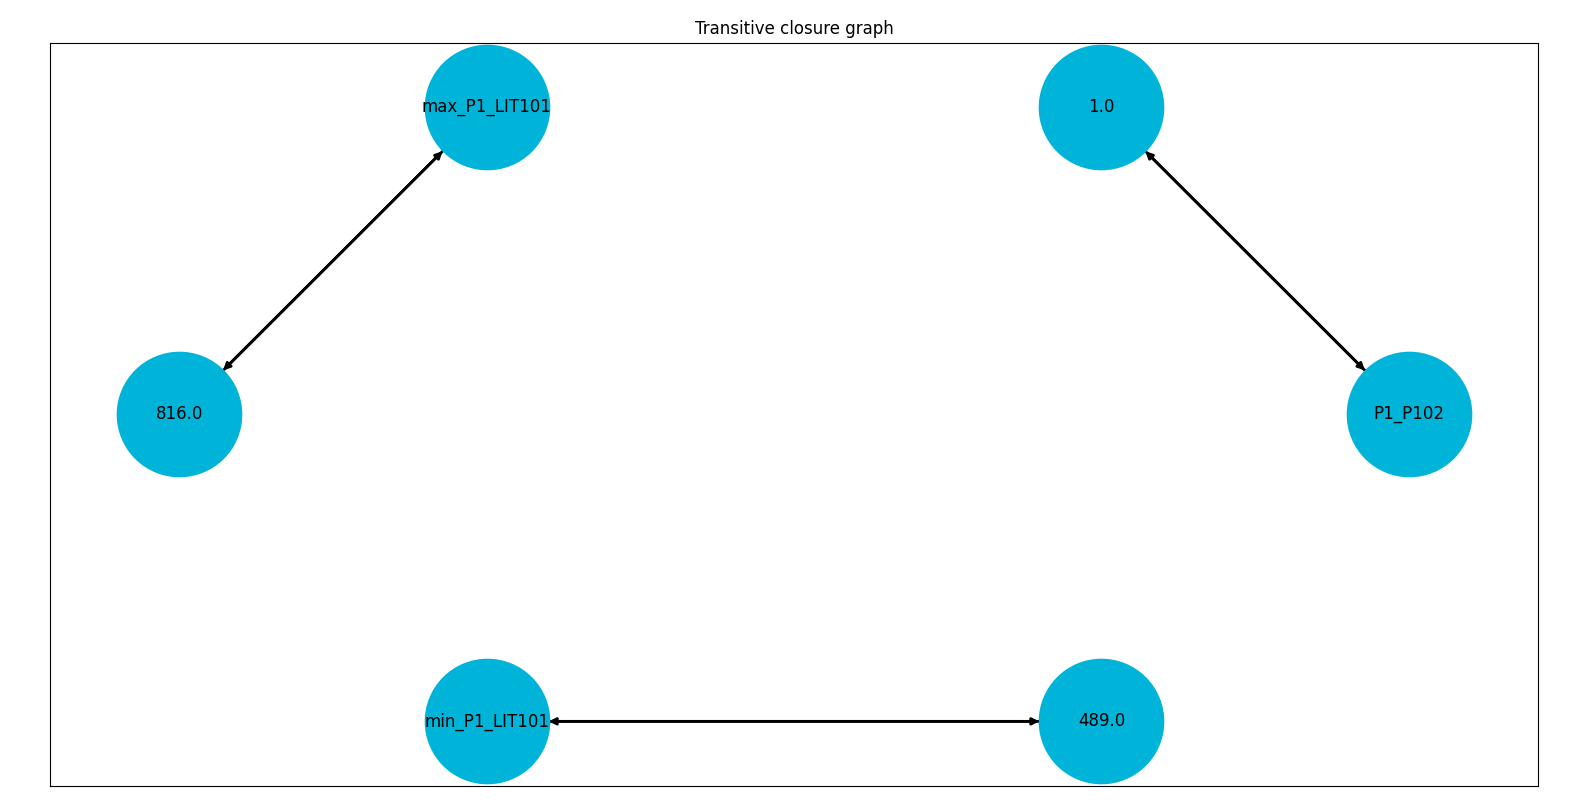
\includegraphics[width=\textwidth]{chap4/transitive_closure_eq.png}
		\caption{Transitive closure graph for "=="}
		\label{subfig:4_graph_eq}
	\end{subfigure}
	\hfill
	\begin{subfigure}{0.48\textwidth}
		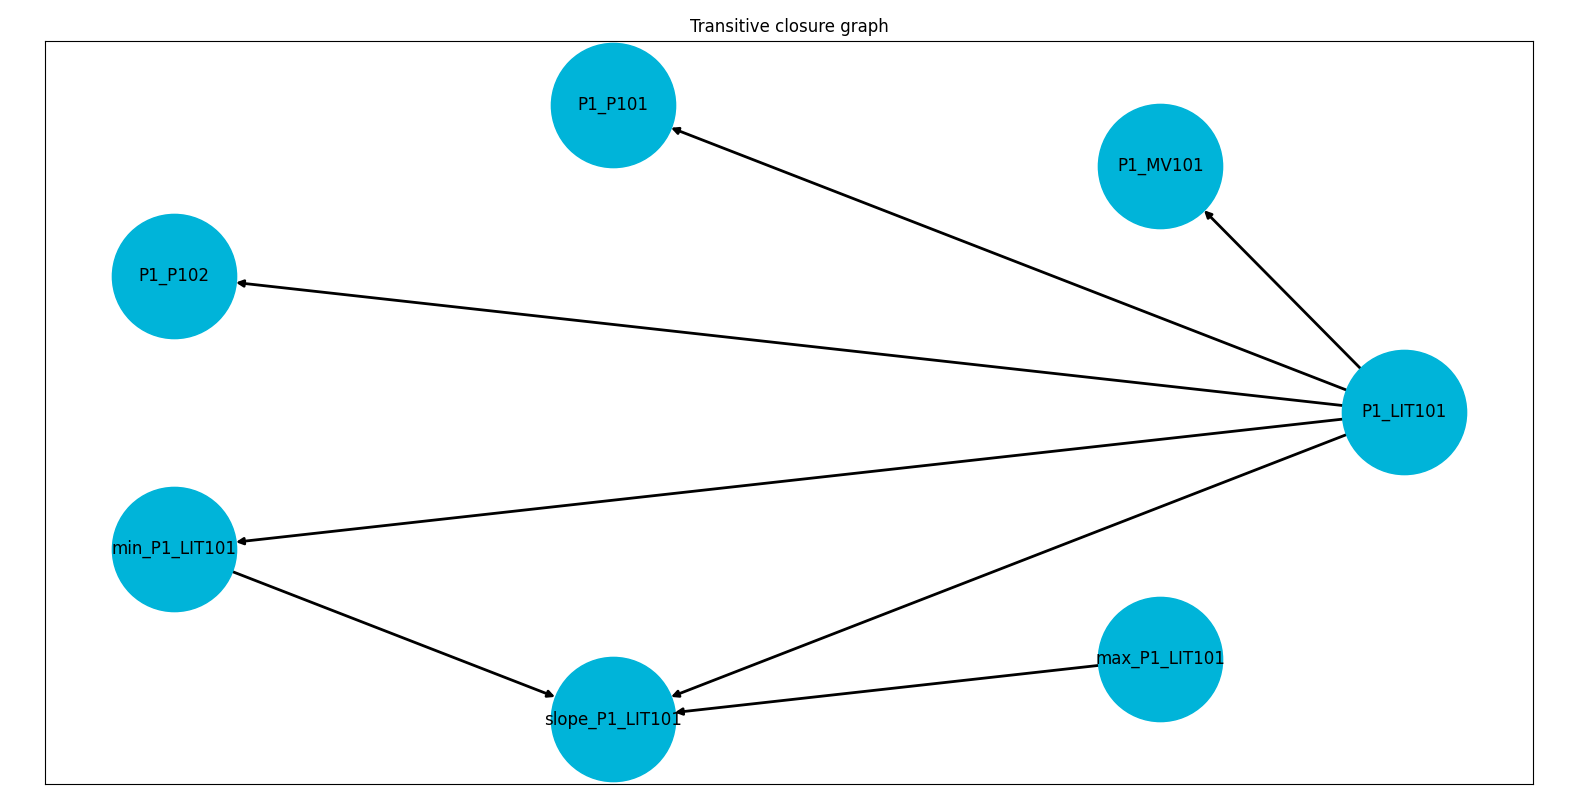
\includegraphics[width=\textwidth]{chap4/transitive_closure_gt.png}
		\caption{Transitive closure graph for ">"}
		\label{subfig:4_graph_gt}
	\end{subfigure}
	\begin{subfigure}{0.48\textwidth}
		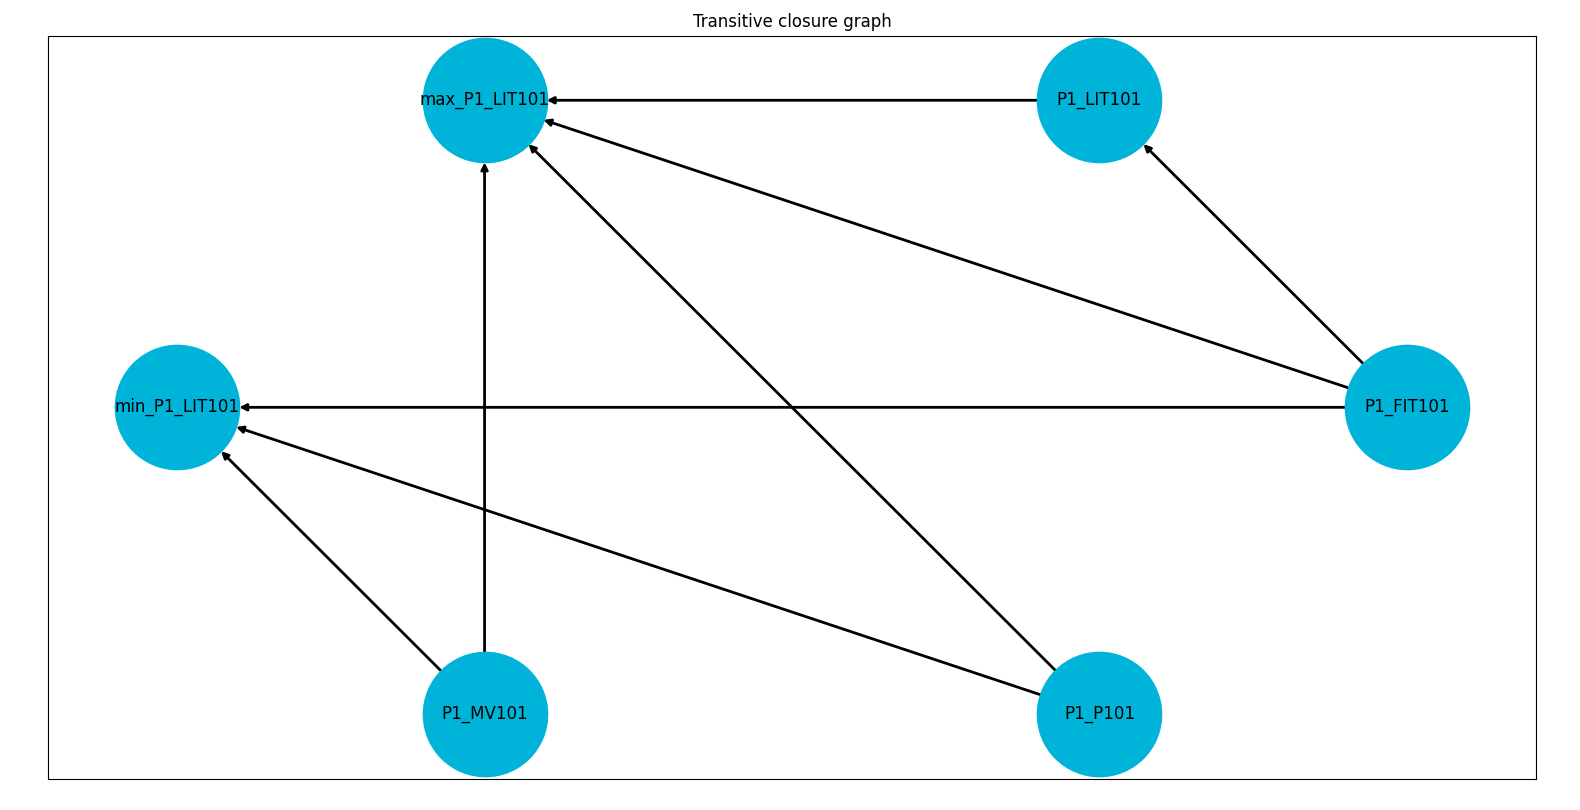
\includegraphics[width=\textwidth]{chap4/transitive_closure_lt.png}
		\caption{Transitive closure graph for "<"}
		\label{subfig:4_graph_lt}
	\end{subfigure}
	\hfill
	\begin{subfigure}{0.48\textwidth}
		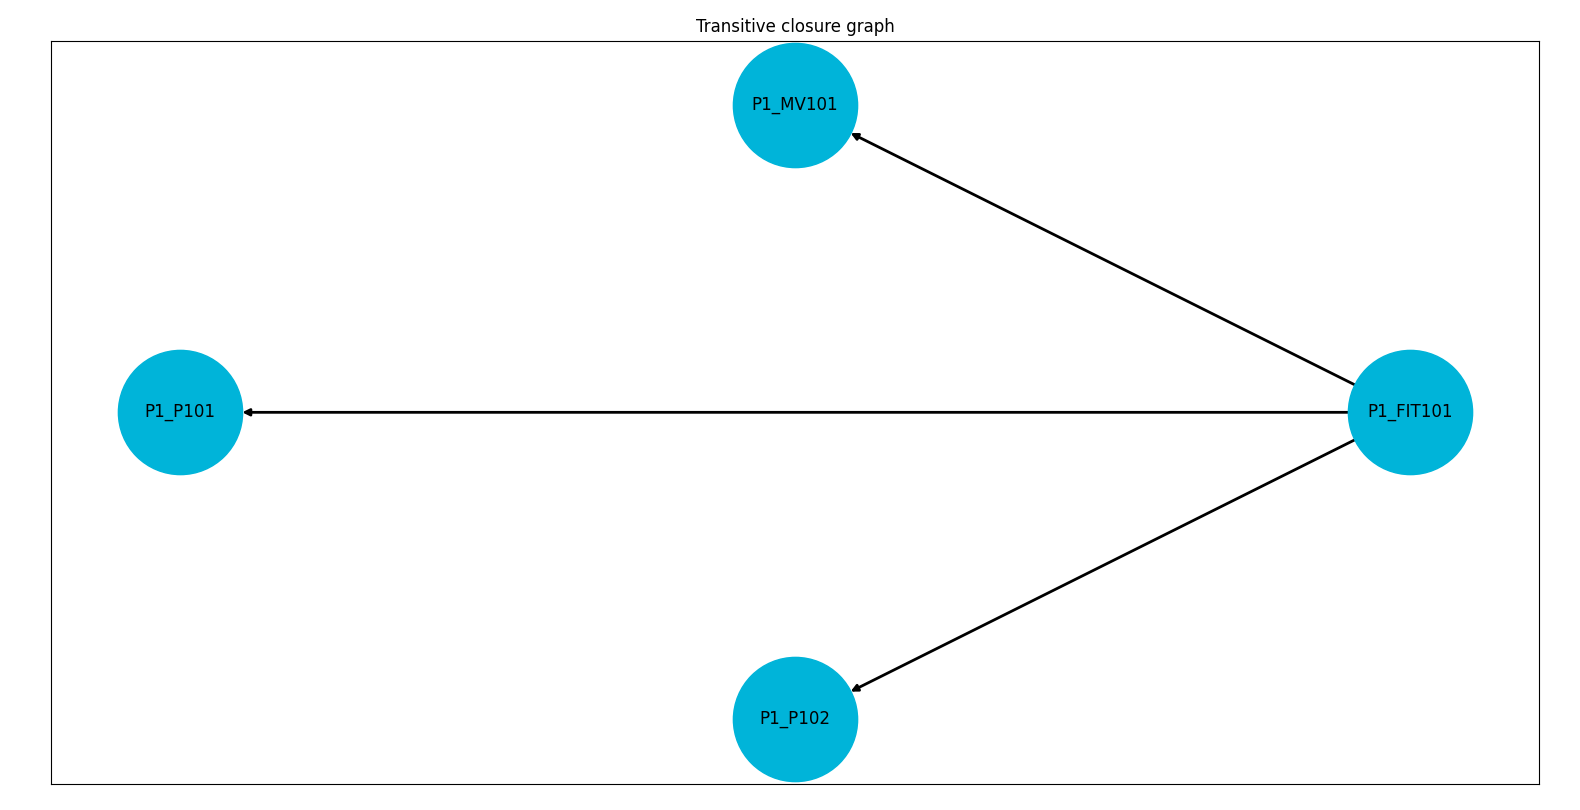
\includegraphics[width=\textwidth]{chap4/transitive_closure_gt_cond.png}
		\caption{Transitive closure graph for ">" cond.}
		\label{subfig:4_graph_gt_cond}
	\end{subfigure}
	\caption{Example of transitive closure graphs for invariants in PLC1 of iTrust SWaT system}
	\label{fig:4_transitive_closure_graphs}
\end{figure}
At the end of this process, still applied to \texttt{PLC1} of the iTrust SWaT system and with the same analysis condition, we get the following complete output:

\begin{lstlisting}[language=bash,numbers=left,caption={Revised Daikon output with transitive closures for \texttt{PLC1} of the iTrust SWaT system},label=lst:4_daikon_new_output_plc1]
	===========================
	Generic
	===========================
	P1_MV101 one of { 0.0, 1.0, 2.0 }
	P1_P101 one of { 1.0, 2.0 }
	slope_P1_LIT101 one of { -1.0, 0.0, 1.0 }
	P1_FIT101 != P1_P101, P1_P102
	P1_P102 == 1.0
	max_P1_LIT101 == 816.0
	min_P1_LIT101 == 489.0
	P1_LIT101 > P1_MV101
	P1_LIT101 > P1_P101
	P1_LIT101 > P1_P102
	P1_LIT101 > min_P1_LIT101 > slope_P1_LIT101
	P1_FIT101 >= 0.0
	P1_P101 >= P1_P102 >= slope_P1_LIT101
	
	===========================
	P1_MV101 == 2.0 && P1_LIT101 < max_P1_LIT101 - 16 && P1_LIT101 > min_P1_LIT101 + 15
	===========================
	slope_P1_LIT101 == P1_P102
	P1_MV101 == 2.0
	P1_FIT101 > P1_MV101
	P1_FIT101 > P1_P101
	P1_FIT101 > P1_P102
	P1_MV101 >= P1_P101
\end{lstlisting}
Transitive closures can be appreciated in lines 7, 14 and 16 of Listing \ref{lst:4_daikon_new_output_plc1}.\newline
In general, the output has been reduced in the number of effective rows (19 versus the 61 in the output of Listing \ref{lst:4_daikon_output_plc1}, making it certainly better to read and identify significant invariants) and the invariant chains make it more immediate to grasp the relationships between registers.

\subsubsection{Types of Analysis}
\label{subsub:4_types_analysis}

Compared to Ceccato et al.'s solution, in which individual analyses are performed manually, my proposal is to implement two types of semi-automated analysis: the first performs an analysis of all states for each individual register, while the second performs the analysis on the current system configuration based on the actual states of the actuators.\newline
Both analyses refer to a specific measurement, selected by the user.

\bigskip
These two types of analysis will be handled by the Python script\\ \texttt{daikonAnalysis.py}, contained in the default directory \texttt{\$(project\_dir)/daikon}.\newline
The script accepts the following command-line arguments:

\begin{itemize}
	\item \textbf{-f} or \textbf{{-}{-}filename}: specifies the enriched dataset, in CSV format, from which to read the data. The dataset must be located within the directory containing the enriched datasets specified in the \textit{config.ini} file (by default \texttt{\$(project\_dir)/daikon/Daikon\_Invariants}).
	
	\item \textbf{-s} or \textbf{{-}{-}simpleanalysis}: performs the analysis on the states of individual actuators
	
	\item \textbf{-c} or \textbf{{-}{-}customanalysis}: performs the analysis on combinations of actual states of the actuators
	
	\item \textbf{-u} or \textbf{{-}{-}uppermargin}: defines a percentage margin on the maximum value of the measurement
	
	\item \textbf{-l} or \textbf{{-}{-}lowermargin}: defines a percentage margin on the minimum value of the measurement
\end{itemize}
One or both types of analysis can be selected. The last two parameters set a condition on the value of the measurement that is meant to bypass the transient periods between the actuator state change and the actual trend change at the maximum and minimum values: this expedient is especially useful for the first type of analysis, allowing for generally more accurate data on measurement trends.

\paragraph{Analysis on single actuator states}
\label{par:4_single_actuator_states_analysis}
Analysis on the states of individual actuators is the simplest: after the user is prompted to input the measurement, chosen from a list of likely available measurements, the script recognizes the likely actuators and the relative states of each, using the same mixed Daikon/Pandas technique adopted in the brief analysis during the pre-processing phase.\newline
For each actuator and each state it assumes, a single Daikon analysis is performed, eventually placing the condition on the maximum and minimum level of the measurement.\newline 
The result of these analyses are saved in the form of text files in a directory having the name corresponding to the analyzed actuator and contained in the default parent directory \texttt{\$(project\_dir)/daikon/Daikon\_Invariants/results}: each file generated by the analysis is identified by the name of the actuator, the state and the condition, if any, on the measurement (see Figure \ref{fig:4_daikon_simpleanalysis_dirfiles}).

\begin{figure}[H]
	\centering
	\begin{subfigure}{0.48\textwidth}
		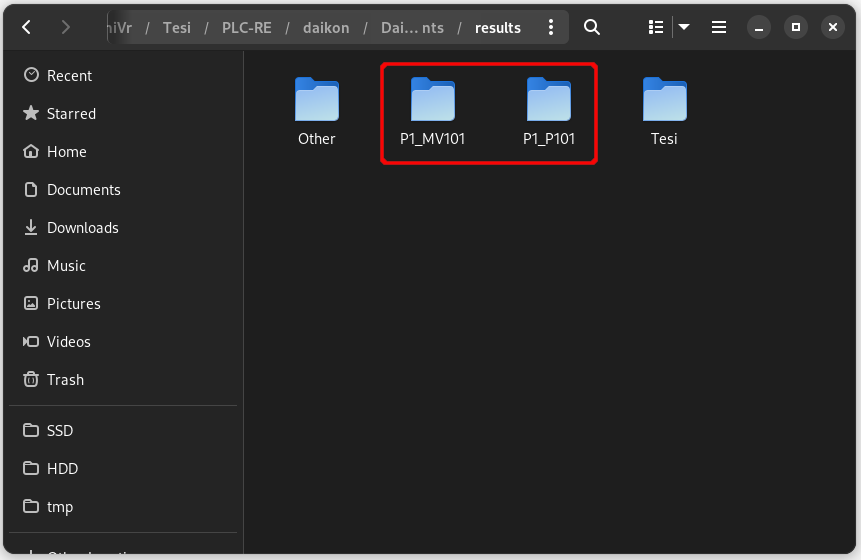
\includegraphics[width=\textwidth]{chap4/daikon_resultfiles_dirs.png}
		\caption{}
		\label{subfig:4_daikon_results_dir}
	\end{subfigure}
	\hfill
	\begin{subfigure}{0.48\textwidth}
		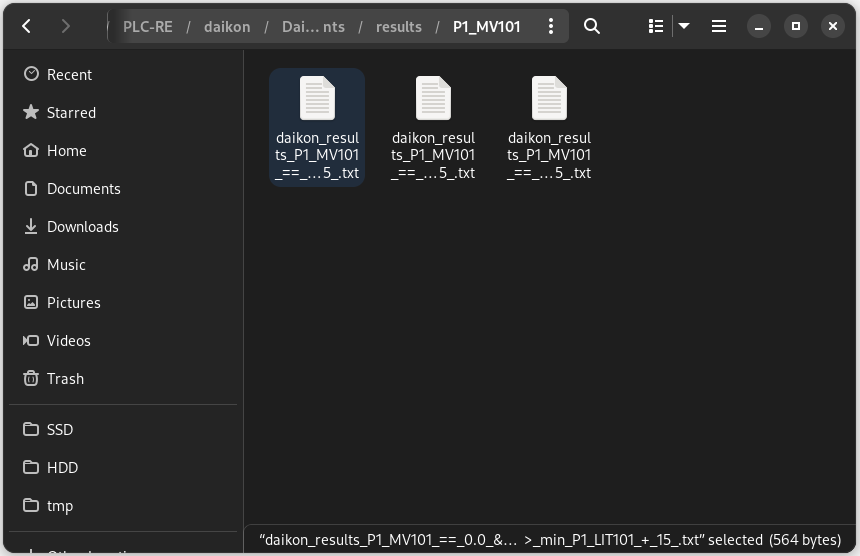
\includegraphics[width=\textwidth]{chap4/actuator_analysis_files.png}
		\caption{}
		\label{subfig:4_daikon_results_file}
	\end{subfigure}
	\caption{Directory (a) and outcome files (b) for the single actuator states analysis}
	\label{fig:4_daikon_simpleanalysis_dirfiles}
\end{figure}

An example of the outcome of this analysis is Listing \ref{lst:4_daikon_new_output_plc1}, where the actuator analyzed is \texttt{P1\_MV101} in state 2: from the generic invariants we can observe that \texttt{P1\_P101} is a likely actuator (line 5), assuming binary values; from line 8, however, we note that \texttt{P1\_P102} is permanently equal to 1, so it can be confirmed that it is a spare actuator rather than a setpoint; furthermore, lines 9 and 10 show the maximum and minimum values reached by \texttt{P1\_LIT101}, which we have assumed to be the register connected to the tank. The most interesting information, however, comes from the condition-generated invariants: at line 21 we notice that the slope of \texttt{P1\_LIT101} is 1 (thus increasing) when \texttt{P1\_MV101} is set to 2: this confirms what we assumed in the previous steps, namely, that \texttt{P1\_MV101} represents the ON state of the actuator and is responsible for filling the tank \texttt{P1\_LIT101}; moreover, at line 23 we see that \texttt{P1\_FIT101} is greater than \texttt{P1\_MV101}: this means that when the actuator assumes the value 2 the sensor \texttt{P1\_FIT101} detects data (in contrast, if \texttt{P1\_MV101} is 1 \texttt{P1\_FIT101} is 0, detecting nothing), confirming the original hypothesis made that this may be a pressure or flow sensor.

\paragraph{Analysis of the Current System Configuration}
\label{par:4_current_system_config_analysis}
The analysis of the current system configuration based on the actual states of the actuators is more complex, but at the same time offers more interesting outcomes as it provides better evidence of actuator behavior in relation to the selected measurement.

\begin{figure}[H]
	\centering
	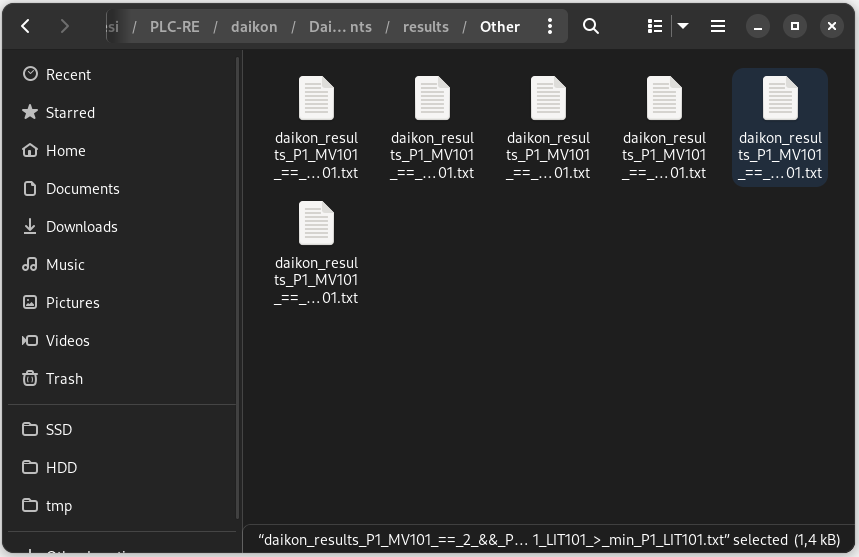
\includegraphics[scale=0.35]{chap4/daikon_systemstate_results.png}
	\caption{Daikon outcome files for system configuration analysis. Each file represents a single system state}
	\label{fig:4_daikon_systemstates_files}
\end{figure}

For this analysis, the script automatically identifies the configurations of the actuators that represent different system states (e.g., \texttt{P1\_MV101 == 2, P1\_P101 == 1}). Daikon analysis is then performed for each of these configurations. The user is prompted to select the measurement attribute and, if desired, specific actuators for studying their configurations. If no actuators are selected, all previously detected actuators will be considered.\newline
The analysis results are saved in text format within a designated directory, located alongside the previous analysis outputs. The filenames of these result files follow a specific naming convention based on the analysis rule applied (see Figure \ref{fig:4_daikon_systemstates_files}).\newline \newline
An example of the obtained outcomes can be seen in Listing \ref{lst:4_current_system_config_analysis}:

\begin{lstlisting}[language=bash,numbers=left,caption={Daikon outcomes for the system configuration \texttt{P1\_MV101 == 2, P1\_P101 == 1} on \texttt{P1\_LIT101}},label=lst:4_current_system_config_analysis]
	===========================
	Generic
	===========================
	P1_MV101 <= P1_P101  ==>  P1_FIT101 >= 0.0
	P1_MV101 <= P1_P101  ==>  P1_MV101 one of { 0.0, 1.0, 2.0 }
	P1_MV101 <= P1_P101  ==>  P1_P101 one of { 1.0, 2.0 }
	P1_MV101 <= P1_P101  ==>  slope_P1_LIT101 one of { -1.0, 0.0, 1.0 }
	P1_MV101 > P1_P101  ==>  P1_FIT101 > P1_MV101
	P1_MV101 > P1_P101  ==>  P1_FIT101 > P1_P101
	P1_MV101 > P1_P101  ==>  P1_FIT101 > P1_P102
	P1_MV101 > P1_P101  ==>  P1_FIT101 > slope_P1_LIT101
	P1_MV101 > P1_P101  ==>  P1_MV101 == 2.0
	P1_MV101 > P1_P101  ==>  P1_MV101 > P1_P102
	P1_MV101 > P1_P101  ==>  P1_MV101 > slope_P1_LIT101
	P1_MV101 > P1_P101  ==>  P1_P101 == 1.0
	P1_MV101 > P1_P101  ==>  P1_P101 == P1_P102
	P1_MV101 > P1_P101  ==>  P1_P101 == slope_P1_LIT101
	P1_MV101 > P1_P101  ==>  slope_P1_LIT101 == 1.0
	[...]
	
	===========================
	P1_MV101 == 2 && P1_P101 == 1 && P1_LIT101 < max_P1_LIT101 && P1_LIT101 > min_P1_LIT101
	===========================
	slope_P1_LIT101 == P1_P102 == P1_P101 == 1.0
	P1_MV101 == 2.0
	P1_FIT101 > P1_MV101
	P1_FIT101 > P1_P101
\end{lstlisting}
Compared to Listing \ref{lst:4_daikon_new_output_plc1}, this time we can observe in the general invariants section the presence of implications, which were previously absent (the remaining generic invariants have been omitted for reasons of space). Such implications can provide very useful information, as in this case: for example, the invariant on line 18 tells us that if the value of \texttt{P1\_MV101} is greater than that of \texttt{P1\_P101} then the value of the slope is 1, that is, the tank level is increasing. Consequently, we have further confirmation that the state \texttt{P1\_MV101 == 2} is the ON state for that actuator and that it is the actuator responsible for filling the tank \texttt{P1\_LIT101}. Comparing the other analysis outcomes, we will discover that \texttt{P1\_P101} is instead responsible for emptying the tank and that its ON and OFF states are 2 and 1, respectively.\newline
In addition, the invariant at line 8 also indicates that when the actuator \texttt{P1\_MV101} is in state 2 and \texttt{P1\_P101} is in state 1 then the value of \texttt{P1\_FIT101} is greater than 2: consequently, it follows that the corresponding sensor is measuring something relative to the tank \texttt{P1\_LIT101}.\newline
The above is confirmed by the invariants related to the analysis condition: at line 24 we have that the slope is indeed equal to 1 (thus increasing) and that \texttt{P1\_FIT101}, at line 26, takes values greater than 2 when \texttt{P1\_MV101} is equal to 2.

\paragraph{Refining the Analysis}
\label{par:4_refining_analysis}
In some cases, it may happen that the outcomes provided by the semi-automated analyses are not satisfactory to the user (e.g., the value of the slope may not emerge clearly) or simply the user wants to investigate a particular aspect of the system in more detail by trying to discover additional invariants that did not emerge previously: in this case, it is possible to run a new and more specific invariant analysis using the Python script \texttt{runDaikon.py}, which allows for more punctual analyses of the system.\newline
The script, also contained in the default directory \texttt{\$(project\_dir)/daikon}, accepts three command-line parameters:

\begin{itemize}
	\item \textbf{-f} or \textbf{{-}{-}filename}: specifies the enriched dataset, in CSV format, from which to read the data. Even in this case, the dataset must be located within the directory containing the enriched datasets
	\item \textbf{-c} or \textbf{{-}{-}condition}: specifies the condition for the analysis, which will be automatically overwritten in the \textit{.spinfo} file. It is possible to specify more than one condition, but it is recommended to use the logical operator \texttt{\&\&}
	\item \textbf{-r} or \textbf{{-}{-}register}: specifies the directory where to save the text file with the outcomes
\end{itemize}
During the execution of this analysis, a single output file is generated, containing the discovered invariants. The user can specify the directory where this file should be saved using the \texttt{-r} command-line option. By default, the file is stored in the directory \texttt{\$(project\_dir)/daikon/Daikon\_Invariants/results}. The output file serves as a record of the identified invariants and can be examined at a later time. 

\bigskip
In conclusion, the integration of these two analysis types, along with the ability to conduct more refined analysis in the future and the enhanced output format of Daikon, significantly enhances the completeness, clarity, and effectiveness of this stage compared to the previous framework.

\subsection{Phase 4: Businness Process Analysis}
\label{subsec:4_improve_bpa}

\subsection{Phase 5: Network Analysis}
\label{subsec:4_network_analysis}

\vfill
\nolinenumbers

%###### CAPITOLO 5 ######%
\chapter{Case study: the iTrust SWaT System}
\label{casestudy}

\linenumbers
\lettrine[lines=2]{H}{aving} introduced the innovative framework and highlighted its potential in the preceding chapter, we now turn our attention to the case study where we will apply this framework. As previously mentioned in Chapter \ref{chap:proposal} and demonstrated through various examples in the same chapter, our focus will be on the \textbf{iTrust SWaT system} \cite{swat_home}, developed by the iTrust -- Center for Research in Cyber Security of University of Singapore for Technology and Design \cite{itrust_site}. The acronym SWaT represents \textit{\textbf{S}ecure \textbf{Wa}ter \textbf{T}reatment}.

\bigskip
The iTrust SWaT system is a testbed that replicates on a small scale a real water treatment plant arises to support research in the area of cyber security of industrial control systems and has been operational since March 2015: it is still being used by students at the University of Singapore for educational and training purposes and is available to organizations to train their operators on cyber physical incidents.

\section{Architecture}
\label{sec:5_swat_architecture}
In contrast to the virtualized testbed discussed in Section \ref{subsec:ceccato_testbed} by Ceccato et al., the iTrust SWaT system is composed entirely of physical hardware components. It encompasses various elements, starting from field devices and extending to PLCs, HMI, SCADA workstations, and the SCADA server (also referred to as the \textit{historian}). The historian is responsible for recording data from field devices for further analysis. In the upcoming sections, we will delve deeper into the architecture of the physical process and the communication network.

\subsection{Physical Process} 
\label{subsec:5_swat_physical_architecture}
The physical process of the SWaT consists of six stages, denoted P1 through P6. These stages are \cite{swat_tecnical_pdf}\cite{swat_tippenhauer}:

\begin{enumerate}
	\item \textbf{taking in raw water:} feeds unfiltered water into the system
	\item \textbf{chemical dosing:} adds chemicals to water useful for initial pretreatment
	\item \textbf{Ultra Filtration (UF) system:} the water is filtered through a semi-permeable membrane (ultrafiltration membrane) using the liquid pressure, effectively capturing impurities and suspended solids, as well as removing bacteria, viruses, and other pathogens present in the water.
	\item \textbf{dechlorination:} removes residual chlorine from disinfected water using ultraviolet lamps
	\item \textbf{Reverse Osmosis (RO):} performs further filtration of the water
	\item \textbf{backwash process:} cleans the membranes in UF using the water produced by RO
\end{enumerate}
Figure \ref{fig:5_swat_architecture_1} shows a graphical representation of the architecture and the six stages of the SWaT system.

\begin{figure}[ht]
	\centering
	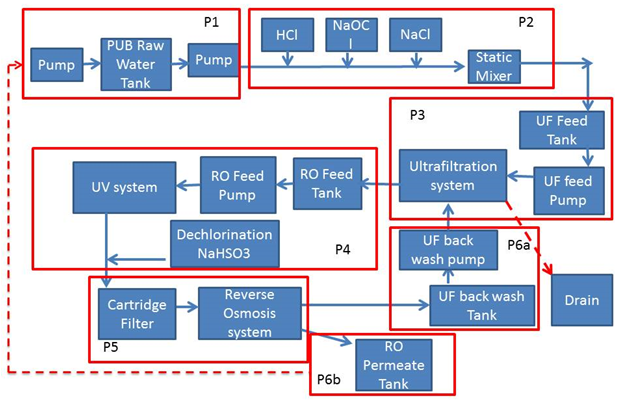
\includegraphics[scale=0.55]{chap5/testbed-3.png}
	\caption{SWaT architecture}
	\label{fig:5_swat_architecture_1}
\end{figure}

\bigskip
The SWaT system incorporates an array of sensors that play a crucial role in monitoring the system's operations and ensuring their safe. These sensors are responsible for continuously collecting data and providing valuable insights into the functioning of the system. These sensors are:

\begin{itemize}
	\item Level Indication Transmitter (measured in mm)
	\item Flow Indication Transmitter (m3/hr)
	\item Analyser Indicator Transmitter
	\begin{itemize}
		\item[o] Conductivity (µS/cm)
		\item[o] pH
		\item[o] Oxidation Reduction Potential (mV)
	\end{itemize}
	\item Differential Pressure Indicator Transmitter (kPa)
	\item Pressure Indicator Transmitter (kPa)
\end{itemize}
The sensors and actuators associated with each PLC are shown in Figure \ref{fig:5_swat_sensors_plc}. \newline
Sensors and actuators are mapped to tags by the communication protocol used (see \ref{subsec:5_swat_network_architecture}): a tag can be addressed via string descriptor defined by the system designer (e.g. MV101, to indicate motorized valve number 1 at stage 1) or by referring directly to the analog/digital pins of the PLC I/O unit \cite{swat_tippenhauer}.

\begin{figure}[ht]
	\centering
	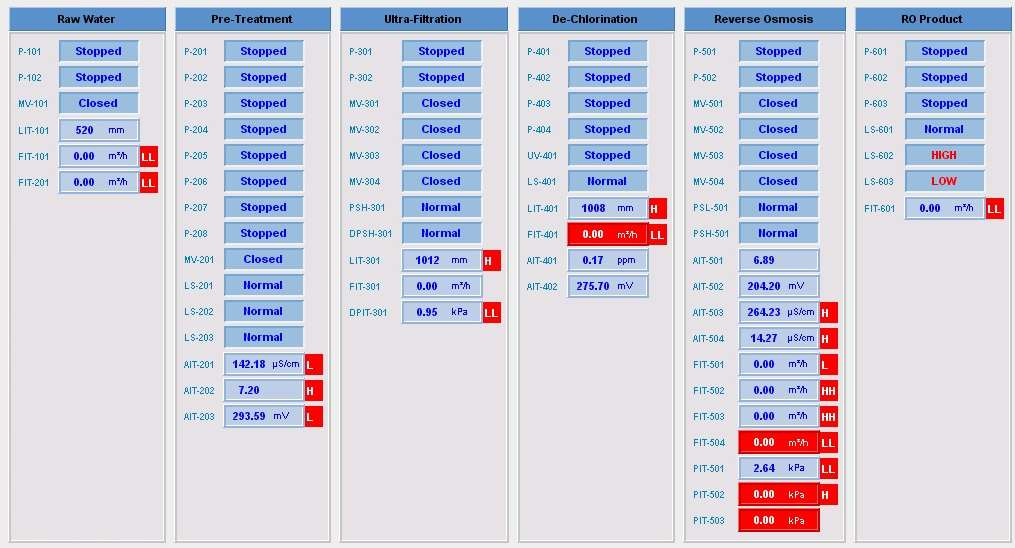
\includegraphics[scale=0.50]{chap5/plc-devices.jpg}
	\caption{Sensors and actuators associated with each PLC}
	\label{fig:5_swat_sensors_plc}
\end{figure}

\subsection{Control and Communication Network}
\label{subsec:5_swat_network_architecture}
The SWaT system's network architecture follows the principles of layering and zoning, which enable segmentation and control of traffic within the network.
\newline \newline
Five layers are present starting from the highest to the lowest: 

\begin{itemize}
	\item \textbf{Layer 3.5} -- Demilitarised Zone (DMZ)
	\item \textbf{Layer 3} -- Operation Management (Historian)
	\item \textbf{Layer 2} -- Supervisory Control (Touch Panel, Engineering Workstation, HMI Control Clients)
	\item \textbf{Layer 1} -- Plant Control Network (PLCs) (Star Network)
	\item \textbf{Layer 0} -- Process (Actuator/Sensors and Input/output modules) (Ring Network)
\end{itemize}
PLCs at Layer 1 communicate with their respective sensors and actuators at Layer 0 through a conventional ring network topology based on EtherNet/IP, to ensure that the system can tolerate the loss of a single link without any adverse impact on data or control functionality.\newline
PLCs between the different process stages at Layer 1 communicate with each other through a star network topology using the CIP protocol on EtherNet/IP, previously discussed in Section \ref{subsubsec:cip}.

\bigskip
Regarding zoning, the SWaT system is divided into three zones, each containing one or more layers. These zones are, in descending order of security level: 

\begin{itemize}
	\item \textbf{Plant Control Network}, or \textbf{Control System:} includes layers from 0 to 2
	\item \textbf{DMZ:} includes Layer 3.5
	\item \textbf{Plant Network:} includes Layer 3
\end{itemize}
Figure \ref{fig:5_swat_network_arch} provides a clearer visualization of the zoning and layer division within the network architecture of the SWaT system. This diagram highlights the distinct zones and their corresponding layers, offering a comprehensive overview of the system's network structure.

\begin{figure}[ht]
	\centering
	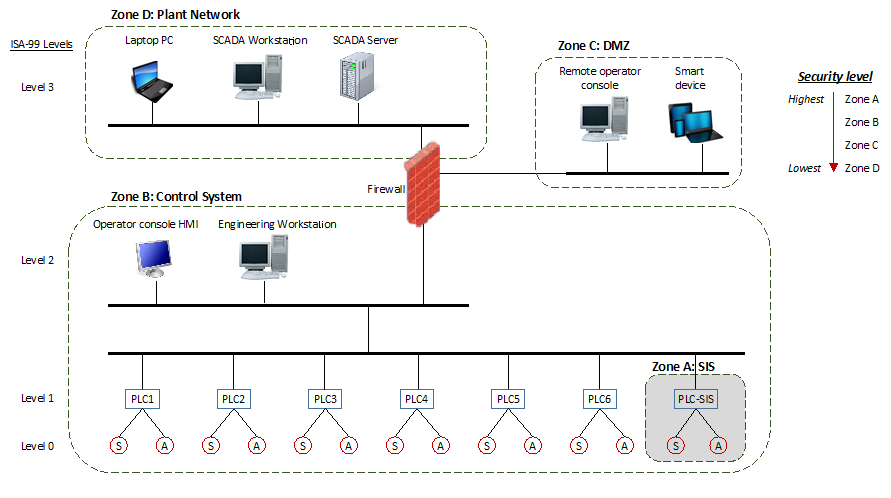
\includegraphics[scale=0.60]{chap5/testbed-4.png}
	\caption{SWaT network architecture}
	\label{fig:5_swat_network_arch}
\end{figure}

\section{Datasets}
\label{sec:5_swat_datasets}

To facilitate the study and testing of technologies related to cyber security in Industrial Control Systems and critical infrastructure, iTrust offers researchers worldwide the opportunity to access a range of datasets \cite{swat_datasets}. These datasets consist of a collection of data obtained from the SWaT system, encompassing information on both the physical processes and network communications. The data is organized into different years, and researchers can request access to these datasets for their analysis and experimentation purposes.

\bigskip
\paragraph{Physical Process Datasets}
The datasets containing information about the physical processes are provided in CSV format files. These files encompass data collected during different time intervals, which can vary from a few hours to entire days. The granularity of the data is typically at a one-second interval, although there may be some exceptions. The collected data primarily consists of timestamped sensor measurements and actuator status values for each PLC, describing the physical properties of the testbed in operational mode.

\paragraph{Network Communications Datasets}
Network communications are typically available in the form of \textit{Packet Capture} format (PCAP) files. These files contain captures of communication network traffic, allowing researchers to analyze and examine the network interactions. In some instances, CSV files are provided instead of PCAP files, featuring different characteristics for the collected data.

\subsection{Our Case Study: the 2015 Dataset}
\label{subsec:5_2015_datasets}
The dataset selected as a case study to apply the framework discussed in the previous chapter is specifically the dataset from the year 2015. The main reason for this choice is the unique characteristics found in the physical process dataset that are not present in datasets from subsequent years.

\paragraph{Physical Process Data}
The data collection process lasted 11 consecutive days, 24 hours per day. During the first 7 days, the system operated normally without any recorded attacks. However, attacks were observed during the remaining 4 days. The collected data reflects the impact of these attacks, leading to the creation of two separate CSV files: one containing the recorded data of SWaT during the system's regular operations, and the other containing data recorded during the days of the attacks. To ensure accurate information about the system, the dataset pertaining to the normal operations, which spans seven days, was chosen for analysis.

\bigskip
Data collection occurs at a frequency of one data point per second, with the assumption that significant attacks cannot occur within a shorter time frame. Additionally, the firmware of the PLCs remains unchanged throughout the data collection period.\newline
At the beginning of data gathering the tanks are empty and the system must be initialized in order to then reach full operation: it typically takes around five hours for all tanks to be fully filled and for the system to stabilize and reach the appropriate operational state.\newline \newline
In total, the dataset consists of more than 900 thousand records related to 51 attributes.

\paragraph{Network Traffic}
The network traffic was collected using an appliance from a well-known network hardware manufacturer and was made available only in CSV format and not PCAP format. Unfortunately, the data provided are partial as it only includes readings from sensors and does not include information on actuator status.

\bigskip
\begin{longtable}[c]{| c | c |}
	\hline
	\textbf{Category} & \textbf{Description} \\ [0.5ex] 
	\hline
	Date & Date of Log \\
	\hline 
	Time & Time of Log \\
	\hline
	Origin & IP of server \\
	\hline 
	Source IP & IP address of source \\ 
	\hline
	Destination IP & IP address of destination \\ 
	\hline
	Protocol & Network protocol \\ 
	\hline
	Application Name & Name of application \\ 
	\hline
	Modbus Function Code & Function Code \\ 
	\hline
	Modbus Function Description & Description of function \\ 
	\hline
	Modbus Transaction ID & Transaction ID \\ 
	\hline
	SCADA Tag & Sensor or actuator ID \\ 
	\hline
	Modbus Value & Value transmitted \\ 
	\hline
	Service / Destination Port & Port number of destination IP \\ 
	\hline
	Source Port & Port number of source IP \\ 
	\hline
	
	\caption{SWaT network traffic data}
	\label{table:5_swat_network_traffic_data}
\end{longtable}

\vfill
\nolinenumbers

%###### CAPITOLO 6 ######%
\chapter[Our Framework at Work on the iTrust SWaT System]{Our Framework at Work: Reverse Engineering of the iTrust SWaT System}
\label{application}
\linenumbers

\lettrine{I}{n this} chapter, our main objective is to apply the framework and methodology introduced in Chapter \ref{chap:proposal} to the case study of the iTrust SWaT system, as illustrated in Chapter \ref{casestudy}. The purpose of this analysis is to assess the effectiveness and potential of the proposed framework within the context of a system that closely replicates a real-world water treatment plant, albeit on a smaller scale.

\bigskip
Due to the complexity of the system and the limited space available in this thesis, we will not conduct a comprehensive analysis and reverse engineering of the entire system. Instead, we will focus on specific parts for analysis. We leave it to the reader or those interested in utilizing the proposed methodology and framework to complete the analysis, should they choose to do so.

By focusing on selective components and leaving room for further exploration, we strike a balance between providing valuable insights and acknowledging the potential for additional research. This approach empowers the reader and interested individuals to explore the iTrust SWaT system further and leverage the proposed methodology and framework for a more comprehensive analysis.

\section{Preliminary Operations}
\label{sec:6_preliminar_operations}
Prior to beginning the actual analysis, several preliminary manual operations need to be conducted on the physical process dataset utilized as a case study, specifically the SWaT system dataset for the year 2015 as outlined in Section \ref{subsec:5_2015_datasets}. To simulate the data-capture process performed by Ceccato et al. using their scanning tool, the original dataset in XLSX format (proprietary to Microsoft Excel) was divided into multiple datasets in CSV format. Each of these datasets corresponds to the individual stages of the SWaT system and contains the respective registers. These resulting files were then saved in the directory specified by the \texttt{raw\_dataset\_directory} directive in the framework configuration file, \textit{config.ini}, ready to be used in the pre-processing phase.
Furthermore, the headers were manually renamed by adding a prefix from \texttt{P1\_} to \texttt{P6\_} to each register's name. This prefix indicates the stages, ensuring that each register is easily identifiable and linked to its corresponding stage.

\section{Planning the Analysis Strategy}
\label{sec:6_analysis_strategy}
The complexity of the system being analyzed necessitates the adoption of a deliberate strategy for the analysis. It is not feasible to rely on trial and error or attempt every possible combination between stages. The former approach may overlook crucial relationships between PLCs or between registers, while the latter may result in excessive and unproductive efforts if the specific portion of the system being analyzed lacks significant information or relationships. 
A sound analysis strategy helps us focus on the important parts of the system, improving the quality of the analysis and leading to better process comprehension. By prioritizing our attention, we can gain a deeper understanding of the crucial components, resulting in more informed decision-making and a comprehensive understanding of the overall processes.

\bigskip
To define this strategy, a potential starting point could involve analyzing network traffic to determine the communication patterns and participants within the system. This can be accomplished by utilizing the techniques discussed in Section \ref{subsec:4_network_analysis} on Network Analysis. By applying the Python script described in that section to the data extracted from the network traffic dataset debated in Section \ref{par:5_2015_net_dataset}, we can generate a (simplified) network graph, as illustrated in Figure \ref{fig:6_network_SWaT}.

\begin{figure}[ht]
	\centering
	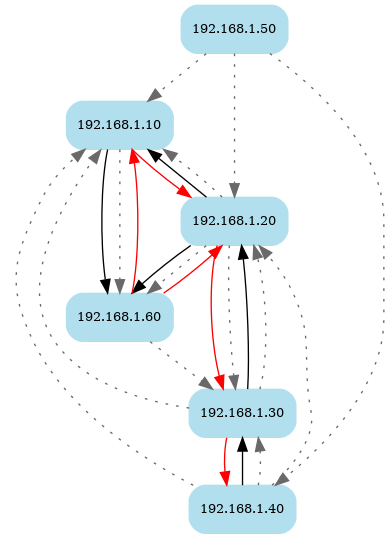
\includegraphics[scale=0.65]{chap6/network2.png}
	\caption{Simplified graph of the iTrust SWaT system network}
	\label{fig:6_network_SWaT}
\end{figure}

The graph clearly illustrates the structure of communications between the PLCs. Referring back to Table \ref{table:5_swat_ip_addresses}, which displays the IP address - PLC associations, we can observe that PLCs 1 through 4 communicate directly and sequentially with each other in a Request/Response communication pattern (represented by red and black arrows, respectively). Additionally, PLC6 communicates with both PLC1 and PLC2. On the other hand, the gray dotted arrows indicate communications for which we have knowledge of a response, but the corresponding request is unknown. For the purposes of our analysis strategy, we will not consider these communications within this context.

\bigskip
Based on our observations, the analysis strategy we will adopt involves considering sequential pairs of PLCs to effectively capture the relationships and implications between registers. %Therefore, the PLC pairs we will focus on are PLC1-2, PLC2-3, and PLC3-4. 

\section{Reverse Engineering of the iTrust SWaT System}
\label{sec:6_reverse_SWaT}
Before we delve into the analysis, it is important to provide some preliminary remarks. 

\paragraph{Analysis structure}
\label{par:6_analysis_struture}
Firstly, the analysis will be structured as a schematic analysis due to space constraints, which prevent us from presenting the extensive inferences and reasoning regarding the system in full detail. Therefore, following the analysis strategy outlined in Section \ref{sec:6_analysis_strategy}, we will concentrate exclusively on the pairs of PLCs comprising PLC1-2, PLC2-3, and PLC3-4. However, the general procedure of the methodology and how to reason about the data obtained from the framework have already been demonstrated through examples on the PLC1 of the SWaT system in Chapter \ref{chap:proposal}. We encourage readers to refer to those examples for a more comprehensive understanding. In this analysis, our focus will be on illustrating the conjectures and properties that arise from the analysis, utilizing tables and the outputs generated during the analysis.

\paragraph{Defining subsystem time duration}
\label{par:6_subsystem_duration}
The second premise addresses the process of defining the subsystems to be analyzed, which were obtained during the pre-processing phase, during the merge phase of the individual datasets. Apart from the projection determined by the considered PLCs, a time-based selection of the analysis period has also been performed (see Section \ref{subsubsec:4_select_subsystem}). This selection spans a duration of 20,000 seconds, which is equivalent to approximately five and a half hours or roughly five system cycles. The analysis begins at 100,000 seconds, which corresponds to approximately 27 hours from the start of the available data. This deliberate selection aims to exclude the initial transient period during which the SWaT system is initialized. We believe that this time range is more than sufficient for accurately defining the characteristics of the SWaT system components.

\paragraph{Conventions}
\label{par:6_conventions}
The third premise introduces a convention that governs the naming of PLC registers and will be consistently followed throughout our analysis. According to this convention, registers with similar names, such as \texttt{P1\_LIT101} and \texttt{P3\_LIT301}, \texttt{P2\_MV201} and \texttt{P3\_MV202}, are considered to belong to the \textbf{same category or type of register}. This convention allows us to establish a relationship or correspondence between registers based on their naming pattern. By grouping registers with similar names, we can infer that they serve similar functions or represent similar components in the system, such as level sensors, tanks, pumps, and so on.

\paragraph{About the Business Process Analysis}
\label{par:6_premesse_bpa}
In the end, the Business Process Analysis will focus solely on the physical process part. This is because the datasets of network traffic captures provided by iTrust for the year 2015 (as discussed in Section \ref{par:5_2015_net_dataset}) are \textbf{incomplete}. While communications related to measurements are present, those associated with actuators are entirely missing, as well as additional communications related to other system characteristics that we observed in the datasets of subsequent years. As a result, we were unable to incorporate the network event recognition component into our Business Process Analysis. To implement this component, we would require complete and overlapping network data, along with a clean physical process dataset not affected by system attacks. Unfortunately, none of the available iTrust datasets fulfill these criteria.

\subsection{Reverse Engineering of PLC1 and PLC2}
\label{subsec:6_P1P2_analysis}
The initial focus of analysis will be on the pair comprising PLC1 and PLC2. Let's delve into the main features of this subsystem by examining the outcomes obtained from applying the framework to it.

\subsubsection{Pre-processing - Preliminary Analysis}
\label{subsubsec:6_P1P2_preprocessing}

\paragraph{Measurements and Actuators Recognition} 
\label{par:6_P1P2_measures_actuators_recognition}
Listing \ref{lst:6_preproc_P1P2} shows the outcomes obtained from automatic recognition of likely measurements and actuators:

\begin{lstlisting}[language=bash, numbers=left, caption=Preliminary analysis outcomes for sensors and actuators of \texttt{PLC1-2}, label=lst:6_preproc_P1P2]
	Actuators: 
	P1_MV101 [0.0, 1.0, 2.0]
	P1_P101 [1.0, 2.0]
	P2_MV201 [0.0, 1.0, 2.0]
	P2_P203 [1.0, 2.0]
	P2_P205 [1.0, 2.0]
	
	Sensors: 
	P1_FIT101 {'max_lvl': 2.7, 'min_lvl': 0.0}
	P1_LIT101 {'max_lvl': 815.1, 'min_lvl': 489.6}
	P2_AIT201 {'max_lvl': 256.5, 'min_lvl': 252.9}
	P2_AIT202 {'max_lvl': 8.4, 'min_lvl': 8.3}
	P2_AIT203 {'max_lvl': 342.8, 'min_lvl': 320.0}
	P2_FIT201 {'max_lvl': 2.5, 'min_lvl': 0.0}
	
	Hardcoded setpoints or spare actuators: 
	P1_P102 [1.0]
	P2_P201 [1.0]
	P2_P202 [1.0]
	P2_P204 [1.0]
	P2_P206 [1.0]
\end{lstlisting}

Based on the results presented in Listing \ref{lst:6_preproc_P1P2}, the framework has identified \texttt{P1\_MV101}, \texttt{P1\_P101}, \texttt{P2\_MV201}, \texttt{P2\_P203}, and \texttt{P2\_P205} as \textbf{probable actuators}. The actuators denoted by the \textit{Pxxx} notation are binary actuators (not boolean!), meaning they have two states represented by the values 1 and 2. Conversely, the actuators identified by the \textit{MVxxx} notation are ternary actuators with three distinct states: 0, 1, and 2. 

To simplify the analysis, we have arbitrarily categorized the registers identified by the notation \textit{MVxxx} as \textbf{valves} and the registers identified by the notation \textit{Pxxx} as \textbf{pumps}. It is important to note that this distinction is solely for convenience and does \textit{not} necessarily reflect the actual role or function of these actuators within the system. 

\bigskip
\texttt{P1\_FIT101}, \texttt{P1\_LIT101}, \texttt{P2\_AIT201}, \texttt{P2\_AIT202}, \texttt{P2\_AIT203}, and \texttt{P2\_FIT201} have been identified as \textbf{likely measurements}. Upon analyzing the range of values for register \texttt{P1\_LIT101}, we observe a significant difference between the maximum and minimum values. This observation leads us to speculate that \texttt{P1\_LIT101} could be identified as a \textbf{level sensor for the tank controlled by PLC1}. However, when examining registers \texttt{P1\_FIT101}, \texttt{P2\_FIT201}, \texttt{P2\_AIT201}, and \texttt{P2\_AIT202}, the small difference between their maximum and minimum values makes it unlikely that they represent additional tanks. 

Regarding register \texttt{P2\_AIT203}, although the range of values is not as wide as in the case of \texttt{P1\_LIT101}, it is still worth examining more closely. It is possible that \texttt{P2\_AIT203} indicates the presence of a small tank. However, considering our speculation that the other \texttt{P2\_AIT20x} registers are not tank level sensors, it is uncertain whether \texttt{P2\_AIT203} falls into that category as well. Further analysis is required to confirm its role within the system.

\bigskip
Some registers have been identified as \textbf{hardcoded setpoints} or \textbf{spare actuators} based on their constant values. These registers exhibit similarities to the previously recognized pump registers. It is plausible to speculate that these registers could correspond to \textbf{spare actuators}. Moreover, the constant value of 1 associated with these registers suggests that it may represent the \textbf{OFF state} of the pumps. 

\paragraph{Actuator State Durations}
\label{par:6_P1P2_actuators_duration}
To gain a deeper understanding of the different states (0, 1, and 2) associated with valves \texttt{P1\_MV101} and \texttt{P2\_MV201}, we can analyze the duration of each state. Listing \ref{lst:6_preproc_P1P2_actuator_duration} provides information regarding the duration (in seconds) of states for these specific actuators:

\begin{lstlisting}[language=bash, numbers=left, caption=Time duration of the states of actuators \texttt{P1\_MV101} and \texttt{P1\_MV201} of PLC1-2, label=lst:6_preproc_P1P2_actuator_duration]
	Actuator state durations:
	P1_MV101 == 0.0
	9  9  10  9  9  10  9  9  10  9
	
	P1_MV101 == 1.0
	1174  1168  1182  1160  1172
	
	P1_MV101 == 2.0
	669  3019  3012  3000  2981
	
	P2_MV201 == 0.0
	8  8  8  9  9  8  9  9  9  9
	
	P2_MV201 == 1.0
	1057  1057  1045  1038  1039
	
	P2_MV201 == 2.0
	120  3135  3144  3127  3109
\end{lstlisting}

It is evident that the duration of \textbf{state 0 is relatively short}, averaging around 8-10 seconds, while the other states have much longer durations. This observation suggests that state 0 of a valve is a \textbf{transient state}, indicating a transitional phase within the valve cycle. However, without further information, it is currently not possible to determine the specific position of state 0 within the overall valve cycle.

\paragraph{Actuator State Changes}
\label{par:6_preproc_P1P2_actuator_state_changes}
Now that we have identified \texttt{P1\_LIT101} as the supposed level sensor of the tank, we can examine the trend of the tank level as the actuators change state. Listing \ref{lst:6_P1P2_preproc_changestate} provides information on the levels of the tank in correlation with the state changes of the \texttt{P1\_P101} pump:

\begin{lstlisting}[language=bash, numbers=left, caption=\texttt{P1\_P101} state changes in relation to \texttt{P1\_LIT101}, label=lst:6_P1P2_preproc_changestate]
	Actuator state changes:
	...
	P1_LIT101  P1_P101  prev_P1_P101
	 536.0356        1             2
	 533.3272        1             2
	 542.1591        1             2
	 534.8581        1             2
	 540.5890        1             2
	      ...      ...           ...
	P1_LIT101  P1_P101  prev_P1_P101
	 813.0031        2             1
	 813.0031        2             1
	 811.8256        2             1
	 812.7283        2             1
	 813.3171        2             1
	      ...      ...           ...
\end{lstlisting}

Based on the speculation that state 1 represents the OFF state of the pump and state 2 represents the ON state, we can analyze the data in Listing \ref{lst:6_P1P2_preproc_changestate}. When pump \texttt{P1\_P101} switches from the ON state to the OFF state, the average level of \texttt{P1\_LIT101} is 535. On the other hand, when \texttt{P1\_P101} goes from the OFF state to the ON state, the average level of \texttt{P1\_LIT101} is 813. These values correspond to the \textbf{minimum and maximum relative setpoints} of \texttt{P1\_P101}, respectively. 

Based on this information, we can infer that pump \texttt{P1\_P101} is responsible for \textbf{emptying the tank}. Moreover, it can be extended to assume that a pump, in general, is responsible for \textbf{water outflow}.

\bigskip
Applying the same analysis to the data for valve \texttt{P1\_MV101}, which is not reported for conciseness, we can speculate that \texttt{P1\_MV101} is responsible for \textbf{filling the tank}. In this case, states 1 and 2 would represent the \textbf{OFF and ON states of the valve}, respectively. The relative setpoints of \texttt{P1\_MV101} are approximately 500 (minimum) and 800 (maximum).
By extending this analysis, we can speculate that a valve, such as \texttt{P1\_MV101}, is responsible for controlling the \textbf{water inflow}.

\bigskip
Regarding the elements controlled by PLC2 and the sensor \texttt{P1\_FIT101}, the analysis does not reveal the presence of another tank. Therefore, we cannot determine the exact role of sensors \texttt{P2\_AIT\textit{20x}}, \texttt{P1\_FIT101} and \texttt{P2\_FIT201} at this point.
However, there is a similarity observed between the relative setpoints of \texttt{P1\_P101} and those of \texttt{P2\_MV201}, \texttt{P2\_P203}, and \texttt{P2\_P205}. These registers exhibit very similar values during state changes, suggesting a potential relationship or similar control behavior between them.

\subsubsection{Graphs and Statistical Analysis}
\label{subsubsec:6_P1P2_graphs}

\begin{figure}[ht]
	\centering
	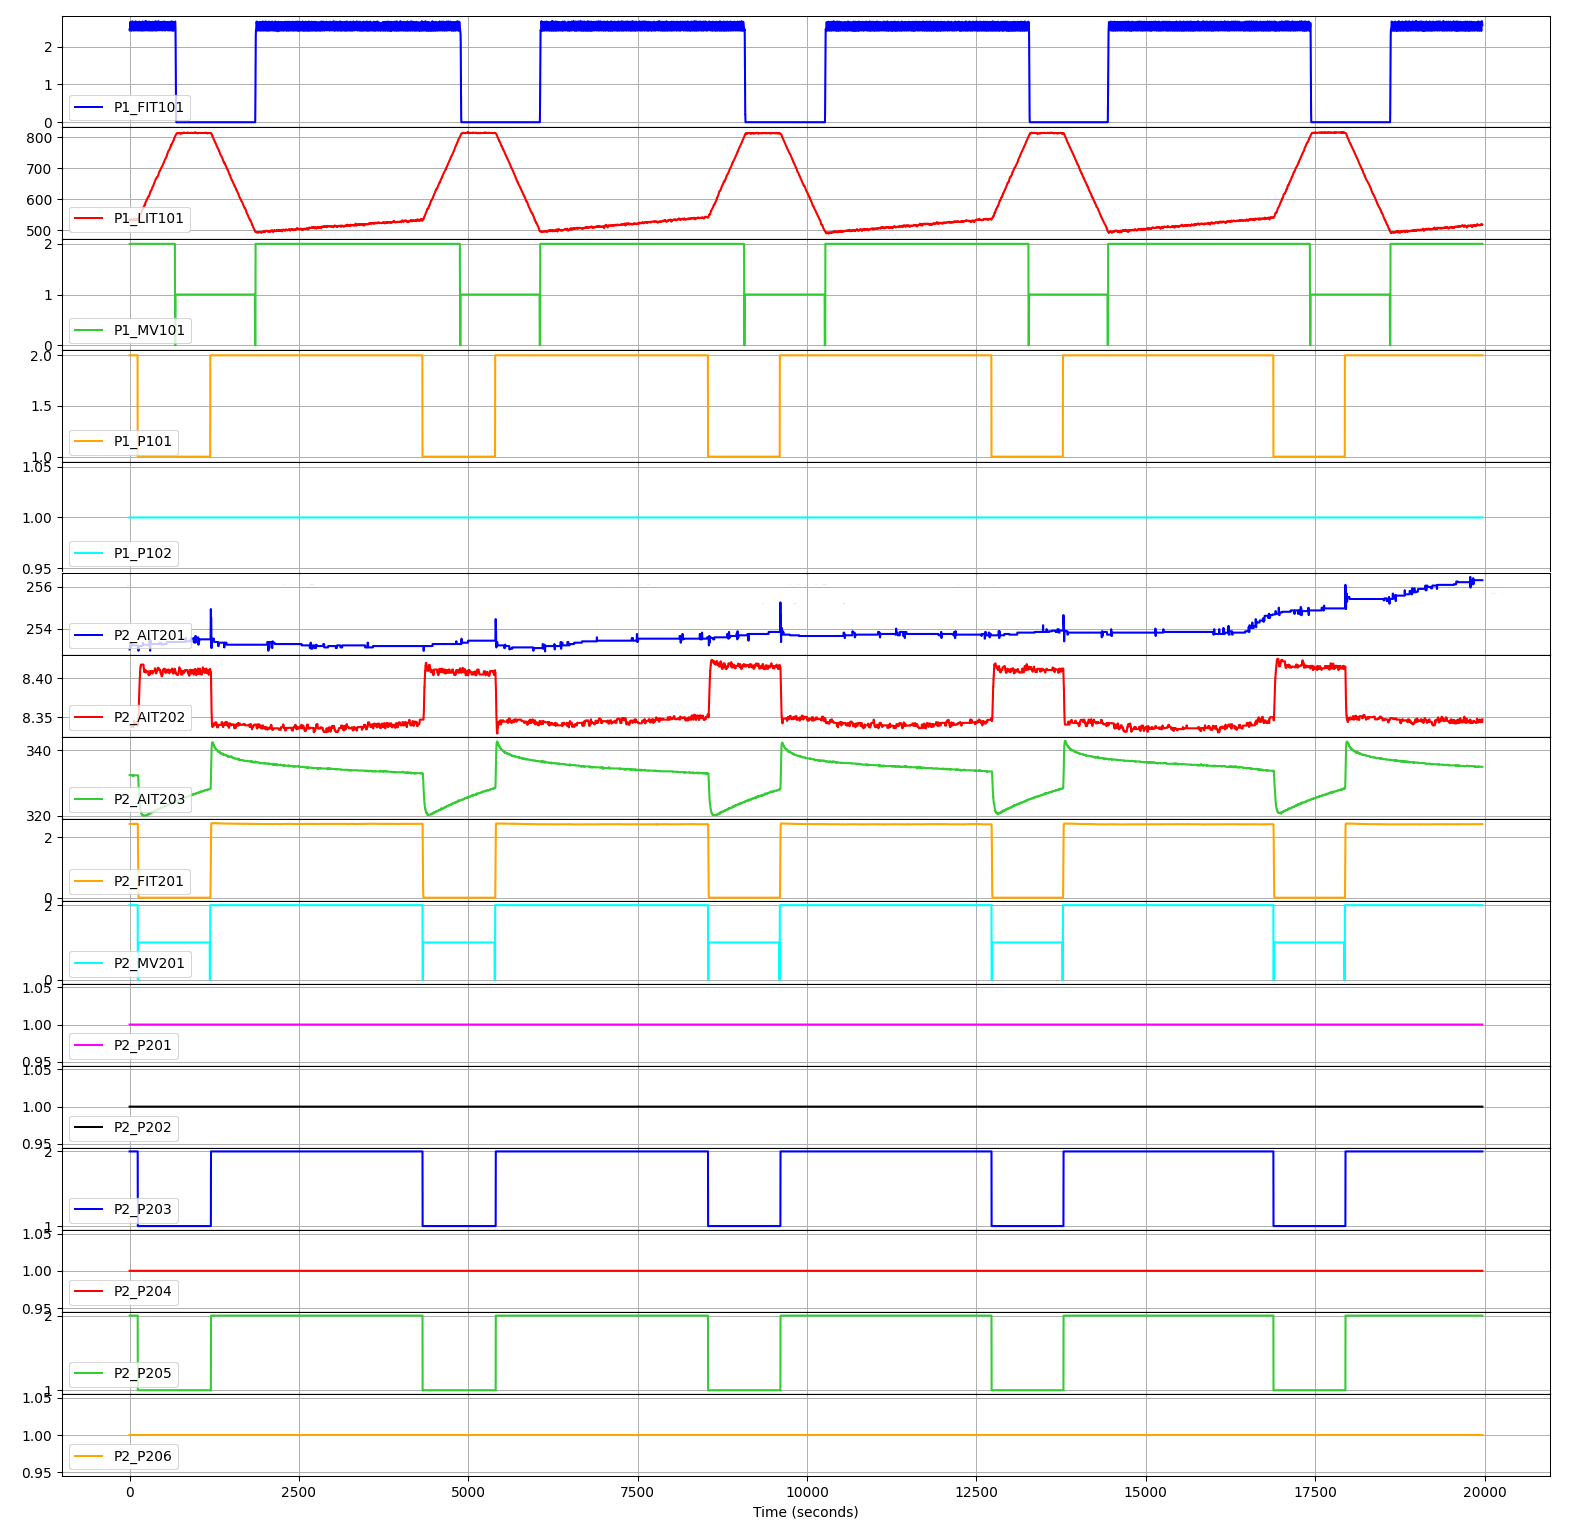
\includegraphics[scale=0.34]{chap6/P1P2_1a.png}
	\caption{Chart of PLC1-2 registers}
	\label{fig:6_P1P2_graph_full}
\end{figure}

Figure \ref{fig:6_P1P2_graph_full} illustrates the graphical representation of the registers in PLC1 and PLC2 and their respective trends.

The image provides additional support to the conjectures made during the preliminary analysis regarding the spare actuators. Furthermore, it is evident from the graphs that these spare actuators \textbf{do not appear to influence the trend} of any of the measurements. Therefore, based on this observation, we can confidently exclude these registers from further graphical analysis.

\bigskip
Figure \ref{fig:6_P1P2_graph_full_nospare} shows a clearer representation of the subsystem after removing the spare actuators.

\begin{figure}[ht]
	\centering
	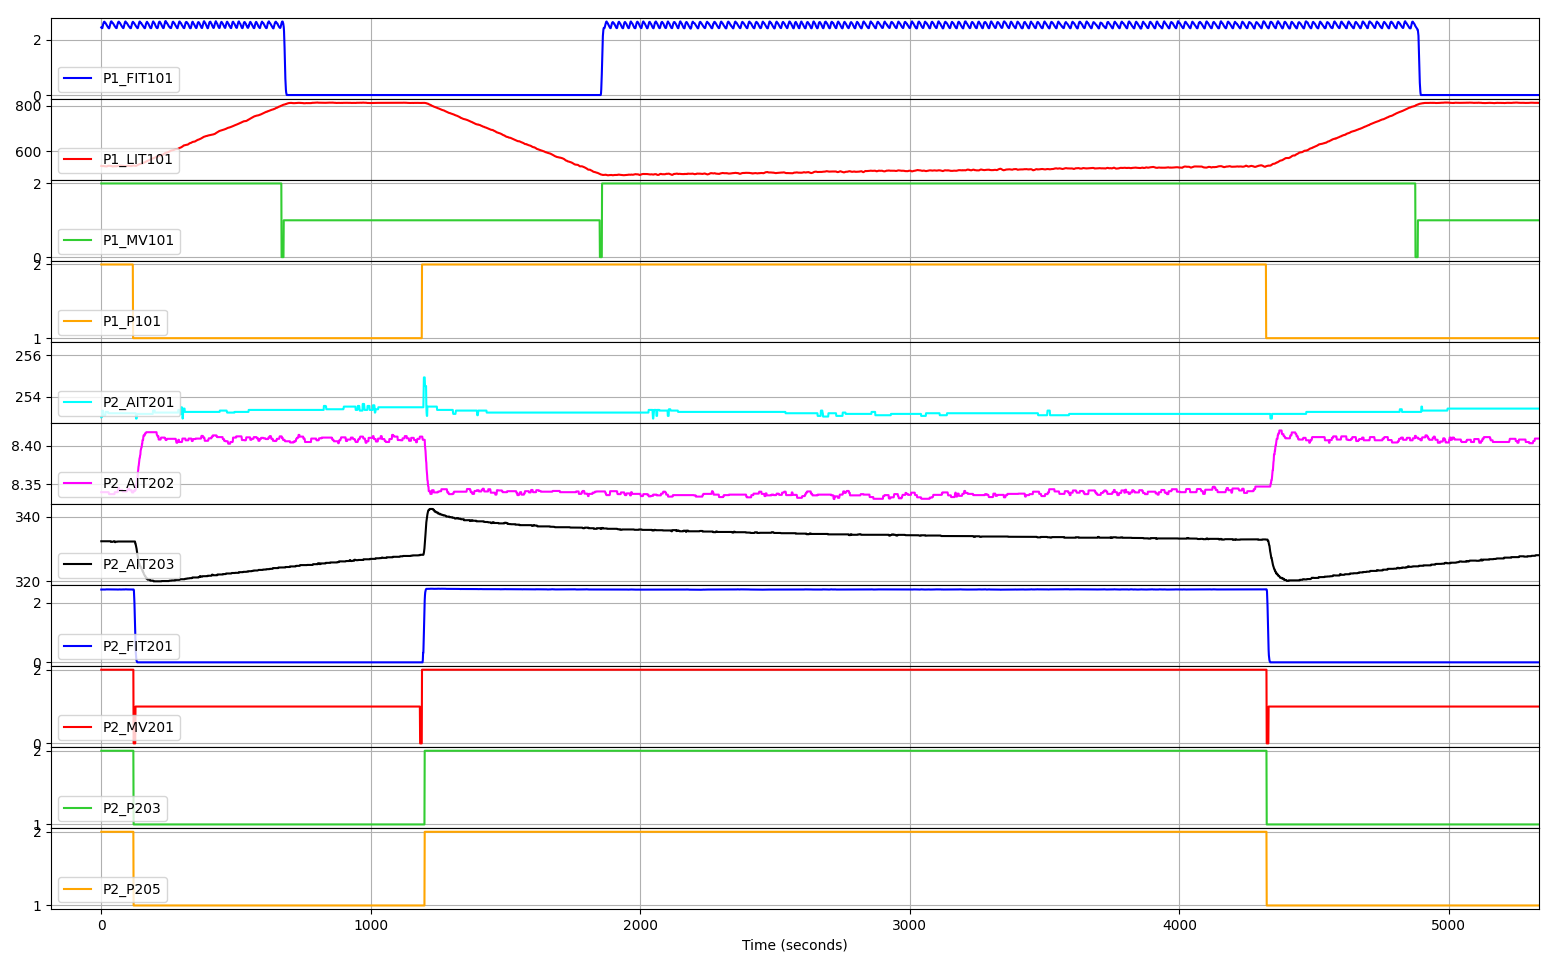
\includegraphics[scale=0.35]{chap6/P1P2_5.png}
	\caption{Chart of PLC1-2 registers without spare actuators (particular)}
	\label{fig:6_P1P2_graph_full_nospare}
\end{figure}

Figure %\ref{fig:6_P1P2_graph_full_nospare} 
provides furthermore additional insights that allow us to speculate on aspects that remained unexplained during the preliminary analysis. The most prominent aspect that stands out is the relationship between the level behavior of \texttt{P1\_LIT101} and the states of \texttt{P1\_P101} and \texttt{P1\_MV101}. It appears evident that these two actuators \textbf{do \textit{not} exhibit complementary behavior}, meaning that their states do not alternate in an \textit{ON-OFF} pattern. Instead, they can remain in the same state, either ON or OFF, for extended periods of time. When they are both in the ON state, \textbf{the growth of the tank level is slow}. However, as soon as \texttt{P1\_P101} switches to the OFF state, the tank level starts to \textbf{increase at a faster rate}. Therefore, when both of these actuators are in the ON state the influx of water into the tank exceeds the outflow of water from it. Conversely, when \texttt{P1\_MV101} switches to the OFF state, the tank level \textbf{decreases}. During periods when both actuators are in the OFF state, there is a \textit{plateau} where the tank level remains relatively \textbf{stable}.

\bigskip
Furthermore, we observe a relationship between \texttt{P1\_FIT101} and the trend of \texttt{P1\_MV101}. When the valve is in the off state, \texttt{P1\_FIT101} registers a value of 0, whereas it registers a value greater than 2 when the valve is open. This suggests that \texttt{P1\_FIT101} could be a \textbf{sensor associated with the flow} of water entering the tank, which is represented by \texttt{P1\_LIT101}. By drawing an analogy with its name, it is plausible to consider \texttt{P2\_FIT201} as another flow sensor.

\bigskip
Another intriguing aspect that arises from examining the graphs in Figure \ref{fig:6_P1P2_graph_full} and Figure \ref{fig:6_P1P2_graph_full_nospare} is the \textbf{non-cyclic pattern} observed in the \texttt{P2\_AIT201} measurement. Instead of exhibiting a cyclical trend, it follows a linear pattern. Furthermore, considering the narrow range of values associated with this measurement, it is reasonable to speculate that \texttt{P2\_AIT201} may be associated with a \textbf{sensor that measures a specific property of the water}.

The limited range of values observed in \texttt{P2\_AIT202} also raises the possibility that it functions as a sensor for a particular water characteristic, despite exhibiting a cyclic pattern. As for \texttt{P2\_AIT203}, its role remains undefined, although it also displays a cyclic trend. This trend, along with that of \texttt{P2\_AIT202}, does not appear to be related to the behavior of the valves (which rules out the possibility of it being related to a tank), but rather to that of the pumps. Consequently, it is imperative to conduct further investigations into these aspects.

\bigskip
By examining the trend of valve \texttt{P2\_MV201}, an additional speculation can be made. It appears to be independent of the trends observed in any of the measurements within this subsystem. Based on previous conjectures regarding the role of valves and considering the duration of its ON and OFF states, it is possible that \texttt{P2\_MV201} is responsible for \textbf{filling a tank that is not part of this particular subsystem}. Once again, a thorough investigation is necessary to confirm this hypothesis.

		
\subsubsection{Invariant Inference and Analysis}
\label{subsubsec:6_P1P2_invariants}
Through the process of \textit{invariant analysis}, we aim to discover new information about the system and determine whether the conjectures made in the previous steps are supported by the data obtained from the Daikon analysis.

\paragraph{General Invariants}
\label{par:6_P1P2_general_invariant}
We will begin this phase by analyzing the general invariants (see Section 4.2.5.1.). Listing \ref{lst:6_preproc_P1P2_general_invariants} presents a selection of these invariants:

\begin{lstlisting}[language=bash, numbers=left, caption=General Invariants for PLC1-2, label=lst:6_preproc_P1P2_general_invariants]
	P2_P206 == P2_P204 == P2_P202 == P2_P201 == P1_P102 == 1.0
	P2_P205 == P2_P203
	max_P1_LIT101 == 816.0
	min_P1_LIT101 == 489.0
	max_P2_AIT201 == 257.0
	min_P2_AIT201 == 252.0
	max_P2_AIT202 == 9.0
	min_P2_AIT202 == 8.0
	max_P2_AIT203 == 343.0
	min_P2_AIT203 == 320.0
\end{lstlisting}

The invariant mentioned on line 2 is particularly significant: it states that \texttt{P2\_P203} and \texttt{P2\_P205} always have the same values. While this information was somewhat apparent in the previous steps, it becomes more apparent and evident in this analysis. This observation leads us to speculate that the two pumps, \texttt{P2\_P203} and \texttt{P2\_P205}, \textbf{are related to each other} in some way. The other invariants provided in this section further reinforce the hypotheses about the spare actuators.

\vfill

\paragraph{Analysis on Single Actuator States}
\label{par:6_P1P2_single_act_states}
We proceed with the examination of the invariants derived from the \textit{first of the two semi-automatic analysis} discussed in Section \ref{par:4_single_actuator_states_analysis}. Specifically, we will focus on the analysis concerning the states of individual actuators in relation to a specific measurement, which in our case pertains to the tank represented by \texttt{P1\_LIT101}. For illustrative purposes, let's consider states 1 and 2 (OFF e ON respectively) of valve \texttt{P1\_MV101} as an example (we will disregard state 0 as it is considered transient). The conditional invariants pertinent to this scenario can be found in Listing \ref{lst:6_preproc_P1P2_conditional_invariants}.

\begin{lstlisting}[language=bash, numbers=left, caption=Conditional Invariants for states 1 and 2 of \texttt{P1\_MV101}, label=lst:6_preproc_P1P2_conditional_invariants]
	===========================
	P1_MV101 == 1.0 && P1_LIT101 < max_P1_LIT101 - 16 && P1_LIT101 > min_P1_LIT101 + 15 
	===========================
	...
	P2_P205 == P2_P203 == P2_MV201 == P1_P101 == 2.0
	P1_FIT101 == 0.0
	slope_P1_LIT101 == -1.0
	P2_FIT201 > P1_FIT101
	P2_FIT201 > P1_MV101
	P2_FIT201 > P1_P101
	...
	
	===========================
	P1_MV101 == 2.0 && P1_LIT101 < max_P1_LIT101 - 16 && P1_LIT101 > min_P1_LIT101 + 15 
	===========================
	slope_P1_LIT101 == P1_P102
	P1_FIT101 > P1_MV101
	...
	P1_MV101 >= P1_P101
	P1_MV101 >= P2_MV201
	P1_MV101 >= P2_P203
	P2_P203 >= P1_P101
	...
\end{lstlisting}

To prevent transient periods caused by water flow stabilization when the actuators change state, a condition is imposed on the level of \texttt{P1\_LIT101}. However, this condition may result in an incomplete understanding of the system's behavior. To address this, a manual refinement of the analysis is required, utilizing the \texttt{runDaikon.py} script as outlined in Section \ref{par:4_refining_analysis}.

\bigskip
Based on the analysis, the following observations can be made when the valve is in the OFF state:

\begin{itemize}
	\item The slope of \texttt{P1\_LIT101}, denoted as \texttt{slope\_P1\_LIT101}, is negative (line 7). This indicates a \textbf{downward trend} in the tank level, as we have seen in Section \ref{par:6_preproc_P1P2_actuator_state_changes}.
	\item \texttt{P1\_P101} is in state 2, or ON (line 5).
	\item \texttt{P1\_FIT101} is zero (line 6).
	\item \texttt{P2\_FIT201} has a value greater than 2 (line 10).
\end{itemize}

\noindent On the other hand, when the valve is in the ON state:

\begin{itemize}
	\item \texttt{slope\_P1\_LIT101} is positive (line 16). This indicates an \textbf{upward trend} in the tank level, as we have seen in Section \ref{par:6_preproc_P1P2_actuator_state_changes}.
	\item \texttt{P1\_FIT101} assumes a value greater than 2. The combination of this finding, along with the previous one regarding the same register, strengthens the hypothesis that this is indeed a flow sensor.
	\item \texttt{P1\_P101} can be in either the ON or OFF state, as we have seen in Section \ref{subsubsec:6_P2P3_graphs}.
\end{itemize}

When conducting a manual analysis using the \texttt{runDaikon.py} script on tank levels that fall outside the range defined by the previous condition, it does not yield useful slope information. This situation can occur because, despite the noise attenuation applied to the tank level sensor data, if there is even a single cycle in the system where the calculated slope deviates from the expected outcome, it can adversely affect the entire Daikon analysis. Figure \ref{fig:6_P1P2_slope_fail} shows this behavior.

\begin{figure}[ht]
	\centering
	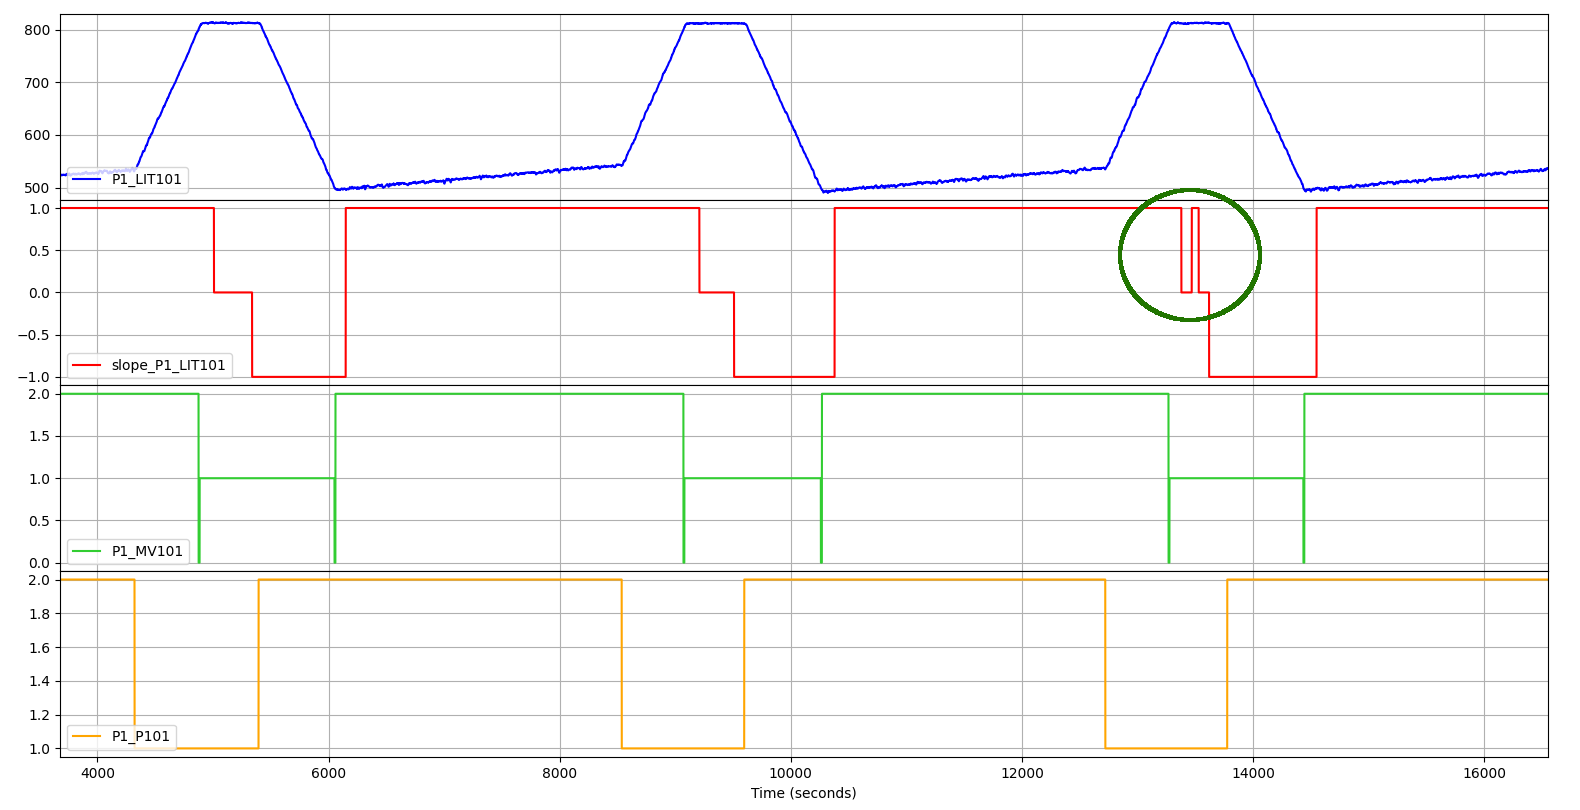
\includegraphics[scale=0.35]{chap6/P1P2_slope_error.png}
	\caption{Slope calculation anomaly (in the circle)}
	\label{fig:6_P1P2_slope_fail}
\end{figure}

\paragraph{Analysis of the Current System Configuration}
\label{par:6_P1P2_current_system_conf}
We conclude our analysis of invariants by considering the \textit{second semi-automatic analysis} outlined in Section \ref{par:4_current_system_config_analysis}, which focuses on the effective states of the system. Due to the comprehensive nature of this analysis, we will not provide a detailed report of the outputs to maintain brevity. However, this analysis confirms the findings observed in the analysis of individual actuator states. Additionally, one crucial piece of information becomes apparent for future steps: the changing state of the actuators controlled by PLC2 \textbf{do \textit{not} impact the behavior of the tank} controlled by PLC1. Indeed, it is sufficient to examine the invariant pertaining to the slope of the tank to verify this observation.


\subsubsection{Business Process Mining and Analysis}
\label{subsubsec:6_P1P2_bpa}
As explained in Section \ref{subsub:4_proc_minining_phy}, the \textit{process mining phase} applied to the physical system provides us with an immediate understanding of the system cycle and the chronological sequence of states. It enables us to determine the duration of time the system remains in a particular state and at what relative setpoint the state transition occurs concerning the reference measure. Furthermore, we can analyze the trend of this measure within each state. Additionally, we can examine the relative setpoints of other measurements to identify any connections between changes in system state and these values. 

\bigskip
Given that we have already identified the likely measurement representing the tank and the corresponding actuators that control its behavior, an activity diagram can be generated as depicted in Figure \ref{fig:6_P1P2_process_mining}.

\begin{figure}[ht]
	\centering
	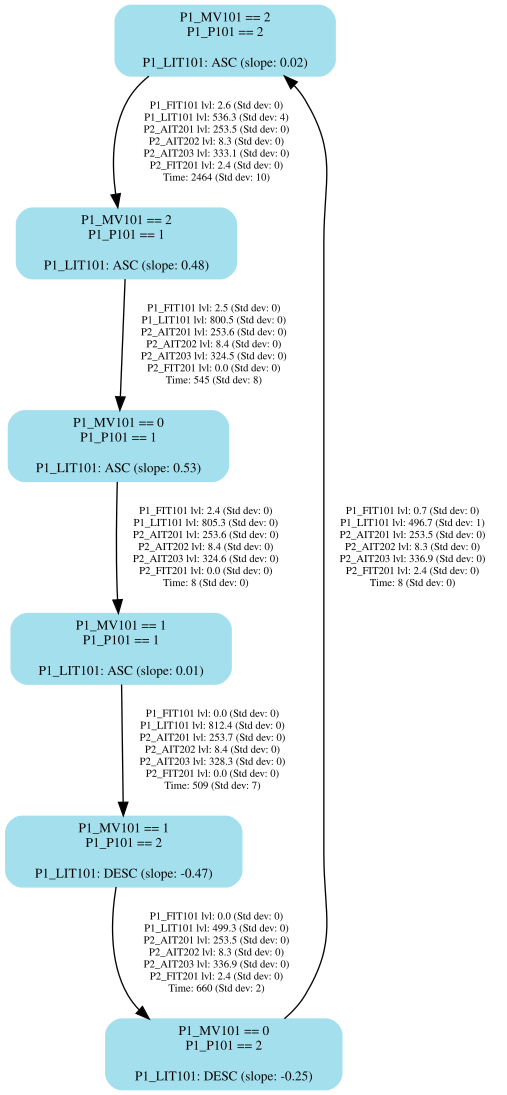
\includegraphics[scale=0.38]{chap6/business_process_P1P2.png}
	\caption{Activity diagram for PLC1-2}
	\label{fig:6_P1P2_process_mining}
\end{figure}

\bigskip
The activity diagram allows for easy interpretation of the tank level trend and slope within different states. The states where the valve has a value of 0 can be disregarded due to their short duration. Similar to the graphical analysis, there is an observed change in slope during the increasing trend of the tank level between the states \texttt{[P1\_MV101 == 2, P1\_P101 == 2]} and \texttt{[P1\_MV101 == 2, P1\_P101 == 1]}, where the slope changes from 0.02 to 0.48.

Additionally, the timing analysis on the edges reveals that the tank takes longer to fill than to empty, and the system remains in the \texttt{[P1\_MV101 == 1, P1\_P101 == 1]} state for approximately 8 minutes (509 seconds).

\bigskip
Regarding the state \texttt{[P1\_MV101 == 1, P1\_P101 == 1]}, there appears to be a discrepancy between the trend of the tank level as reported in the activity diagram and the conjectures made in the previous phases of the analysis. The activity diagram correctly depicts an increasing trend in the tank level between the end of the state \texttt{[P1\_MV101 == 2, P1\_P101 == 1]} and the end of the state \texttt{[P1\_MV101 == 1, P1\_P101 == 1]}. However, the discrepancy arises due to the fact that the interruption of flow during the valve state change from state ON to state OFF is not immediate, mainly due to the presence of the transient state 0. Additionally, water continues to flow within the piping towards the tank for a short duration even after the valve is closed. After this period, which usually lasts a few seconds, the tank level stabilizes, and there is no further inflow or outflow of water. 

By adjusting the tolerance parameter \texttt{-t} in the \texttt{processMining.py} script, it is possible to obtain accurate data regarding the behavior of the state corresponding to the \textit{plateau} observed in the graphical analysis.

\bigskip
The data presented on the arcs in the activity diagram represents the measurement values relative to the time of system state changes, specifically the relative setpoints. These values are calculated based on the average data collected in each cycle. By analyzing this data, we can observe the tank level values at which the system undergoes configuration changes and how the trend of the tank level changes accordingly. Specifically, we can see that the trend changes from ascending to stable at a tank level value of 800, from stable to descending at approximately 812, and from descending back to ascending at around 499. The change in the speed of tank filling occurs at approximately 535.

\bigskip
Furthermore, the data provides additional support for the hypothesis that the measurements associated with registers \texttt{P2\_AIT20x} are not influenced by the tank's trends.

\subsubsection{Properties}
\label{subsubsec:6_P1P2_summary_table}
From the conjectures derived from the four phases of the analysis we will derive the properties of the subsystem we are studying, which will be placed within a \textbf{summary table}. This table contains an integer identifying the property, the statement of the property itself, and from which of the four phases it was derived.

\bigskip
{\footnotesize
	\begin{longtable}[l]{p{0.05\textwidth} p{0.57\textwidth} p{0.30\textwidth}}
		\hline
		\textbf{\#} & \textbf{Statement} & \textbf{Derived from} \\
		\hline
		
		P1 & The registers \texttt{P1\_LIT101}, \texttt{P1\_FIT101}, \texttt{P2\_AIT201}, \texttt{P2\_AIT202}, \texttt{P2\_AIT203}, and \texttt{P2\_FIT201} hold likely sensor measurements. & Preliminary Analysis\newline Graphical Analysis\\
		\hline
		
		P2 & The registers \texttt{P1\_MV101}, \texttt{P1\_P101}, \texttt{P2\_MV201}, \texttt{P2\_P203}, and \texttt{P2\_P205} holds likely actuator commands. & Preliminary Analysis\newline Graphical Analysis\\
		\hline
		
		P3 & The actuators that contain the substring "MVxxx" are considered to be three-state actuators. For simplicity, we refer to them as valves. & Preliminary Analysis\\
		\hline
		
		P4 & The state 0 of these valves is associated to a transient state that occurs during the transition between state 1 (OFF) and state 2 (ON). & Preliminary Analysis\newline Graphical Analysis\\
		\hline
		
		P5 & The actuators that contain the substring "Pxxx" are considered to be binary actuators. For simplicity, we refer to them as pumps. & Preliminary Analysis \\
		\hline
		
		P6 & The registers \texttt{P1\_P102}, \texttt{P2\_P201}, \texttt{P2\_P202}, \texttt{P2\_P204}, and \texttt{P2\_P206} are associated to spare actuators. They do \textit{not} influence the trend of any measurements and they are considered in the OFF state. & Preliminary Analysis\newline Graphical Analysis\newline Invariant Analysis \\
		\hline
		
		P7 & \texttt{P1\_LIT101} is associated to the level sensor of the tank controlled by PLC1. & Preliminary Analysis\newline Graphical Analysis\\
		\hline
		
		P8 & \texttt{P1\_MV101} and \texttt{P1\_P101} are the actuators responsible for the level behavior of the water contained in the tank. & Graphical Analysis\newline Invariant Analysis\newline Business Process\\
		\hline
		
		P9 & \texttt{P1\_MV101} is responsible for filling the tank. \texttt{P1\_P101} is responsible for emptying the tank. & Graphical Analysis\newline Invariant Analysis\\
		\hline
		
		P10 & Valve are responsible for water inflow. Pumps responsible for water outflow. & Preliminary Analysis\newline Graphical Analysis\newline Invariant Analysis\\
		\hline
		
		P11 & The rate of tank level growth is slow when both \texttt{P1\_MV101} and \texttt{P1\_P101} are in the ON state. The growth speed increases when \texttt{P1\_P101} switches to the OFF state. & Graphical Analysis\newline Business Process\\
		\hline
		
		P12 & When both \texttt{P1\_MV101} and \texttt{P1\_P101} are in the ON state, the inflow of water into the tank surpasses the outflow of water from the tank. & Graphical Analysis\newline Business Process\\
		\hline
		
		P13 & The tank level decreases when \texttt{P1\_MV101} is in the OFF state and \texttt{P1\_P101} is in the ON state. & Graphical Analysis\newline Invariant Analysis\\
		\hline
		
		P14 & The tank level remains (relatively) stable when both \texttt{P1\_MV101} and \texttt{P1\_P101} are in the OFF state. & Graphical Analysis\newline Business Process\\
		\hline
		
		P15 & The trend of the tank level changes from ascending to stable when the level reaches approximately 800. It shifts from stable to descending when the level averages around 812. It changes from descending back to ascending when the level reaches about 500. The speed of tank filling increases noticeably at around 535. & Business Process \\
		\hline
		
		P16 & Absolute setpoints are 800, 812, 500 and 535. & Business Process \\
		\hline
		
		P17 & \texttt{P1\_FIT101} serves as a flow or pressure sensor to measure the inflow or the pressure of water into the tank. & Graphical Analysis\newline Invariant Analysis\newline Business Process \\
		\hline
		
		P18 & None of the actuators connected to PLC2 have an impact on the level of the tank controlled by PLC1. & Graphical Analysis\newline Invariant Analysis\newline Business Process \\
		\hline
		
		P19 & None of the measurements connected to PLC2 represent a tank. & Preliminary Analysis\newline Graphical Analysis\\
		\hline
		
		P20 & \texttt{P2\_AIT201} does not exhibit a cyclic trend. & Graphical Analysis\\
		\hline
		
		P21 & Both \texttt{P2\_AIT201} and \texttt{P2\_AIT202} serve as sensors for measuring certain properties of the water. & Preliminary Analysis\newline Graphical Analysis\\
		\hline
		
		P22 & The behavior and trend of \texttt{P2\_AIT202} and \texttt{P2\_AIT203} are directly associated with the operation of the pumps. & Graphical Analysis\newline Invariant Analysis\\
		\hline
		
		\caption{Properties of the PLC1-2 subsystem}
		\label{table:6_P1P2_summarize_properties}
	\end{longtable}
}

\subsection{Reverse Engineering of PLC2 and PLC3}
\label{subsec:6_P2P3_analysis}
Continuing our analysis of the iTrust SWaT system, our current focus will be on the registers of PLC3 and any potential relationships they may have with the registers of PLC2.

\subsubsection{Pre-processing - Preliminary Analysis}
\label{subsubsec:6_P2P3_preprocessing}

\paragraph{Measurements and Actuators Recognition}
\label{par:6_P2P3_measures_actuators_recognition}
Listing \ref{lst:6_preproc_P2P3} shows the outcomes obtained from automatic recognition of likely measurements and actuators. After previously identifying the measurements and actuators of PLC2 in Section \ref{par:6_P1P2_measures_actuators_recognition}, the listing exclusively showcases the registers associated with PLC3.

\begin{lstlisting}[language=bash, numbers=left, caption=Preliminary analysis outcomes for sensors and actuators of \texttt{PLC2-3}, label=lst:6_preproc_P2P3]
	Actuators: 
	...
	P3_MV301 [0.0, 1.0, 2.0]
	P3_MV302 [0.0, 1.0, 2.0]
	P3_MV303 [0.0, 1.0, 2.0]
	P3_MV304 [0.0, 1.0, 2.0]
	P3_P302 [1.0, 2.0]
	
	Sensors: 
	...
	P3_DPIT301 {'max_lvl': 20.4, 'min_lvl': 0.0}
	P3_FIT301 {'max_lvl': 2.4, 'min_lvl': 0.0}
	P3_LIT301 {'max_lvl': 1014.5, 'min_lvl': 786.5}
	
	Hardcoded setpoints or spare actuators: 
	...
	P3_P301 [1.0]
\end{lstlisting}

From the provided listing, it is evident that the \textbf{likely measurements} related to PLC3 are \texttt{P3\_DPIT301}, \texttt{P3\_FIT301}, and \texttt{P3\_LIT301}. Drawing an analogy with the derived properties from Table \ref{table:6_P1P2_summarize_properties}, \texttt{P3\_LIT301} can be associated with a \textbf{tank level sensor}, while \texttt{P3\_FIT301} may be linked to a flow or pressure sensor. However, the specific role of \texttt{P3\_DPIT301} cannot be speculated upon at this time.

\bigskip
Regarding the \textbf{likely actuators}, they include \texttt{P3\_MV301}, \texttt{P3\_MV302}, \texttt{P3\_MV303}, \texttt{P3\_MV304}, and \texttt{P3\_P302}. By drawing parallels with the previous analysis outcomes, it can be inferred that registers \texttt{P3\_MV30x} represent valves, while \texttt{P3\_P302} corresponds to a pump.

\bigskip
Lastly, there is a \textbf{spare actuator} identified as \texttt{P3\_P301}. Similar to the previous analysis, this is an inactive pump, indicated by the constant value of 1 in this register, signifying that it is in the OFF state.

\paragraph{Actuator State Durations}
\label{par:6_P2P3_actuators_duration}
Let's proceed with the analysis of the actuator states' duration, as displayed in Listing \ref{lst:6_preproc_P2P3_actuator_duration}. In this analysis, our focus will not be on examining the correspondence between values and the actual actuator states, as in Section \ref{par:6_P1P2_actuators_duration}. Instead, we will explore whether these actuators exhibit any distinct patterns or behaviors based on their duration.

\begin{lstlisting}[language=bash, numbers=left, caption=Time duration of the states of actuators of PLC3, label=lst:6_preproc_P2P3_actuator_duration]
	Actuator state durations:
	...
	P3_MV301 == 1.0
	2527  4154  4154  4154  4094
	
	P3_MV301 == 2.0
	36  35  36  35  34
	
	P3_MV302 == 1.0
	662  138  654  138  656  139  658  137  656  137
	
	P3_MV302 == 2.0
	62  1783  1596  1787  1591  1791  1576  1803  1540  1782
	
	P3_MV303 == 1.0
	2526  4089  4088  4089  4028
	
	P3_MV303 == 2.0
	97  96  97  96  96
		
	P3_MV304 == 1.0
	689  1832  2206  1838  2203  1840  2191  1852  2152  1831
	
	P3_MV304 == 2.0
	43  87  42  89  43  88  43  88  43  88
	
	P3_P302 == 1.0
	637  115  632  115  632  114  634  114  632  115
	
	P3_P302 == 2.0
	60  1821  1632  1825  1629  1829  1615  1841  1578  1820
\end{lstlisting}

A notable behavior is observed in the \texttt{P3\_MV30x} valves. \texttt{P3\_MV301}, \texttt{P3\_MV303}, and \texttt{P3\_MV304} have a relatively \textbf{short duration in the ON state}, ranging from around 30 seconds to a minute and a half. In contrast, \texttt{P3\_MV302} remains in the ON state for a longer duration but exhibits approximately twice as many cycles as the other actuators (10 cycles compared to 5 cycles). A similar characteristic is also observed in the OFF state of these actuators.

This behavior displayed by the actuators warrants further investigation in subsequent steps. However, based on the short duration of the ON state for \texttt{P3\_MV301}, \texttt{P3\_MV303}, and \texttt{P3\_MV304}, \textbf{it appears unlikely that they have a significant impact on the tank level}. On the other hand, the influence of \texttt{P3\_MV302} cannot be ruled out and requires additional examination.

\bigskip
We can observed that \texttt{P3\_P302}, the pump in PLC3, exhibits a behavior similar to \texttt{P3\_MV302}, with a number of cycles equal to 10. Furthermore, the durations of the ON and OFF states for both actuators appear to be overlapping. This suggests a \textbf{potential relationship between the two actuators}. Additionally, considering that \texttt{P3\_P302} is the only pump in PLC3, it is reasonable to speculate that it may have an influence on the tank level. Further investigation is necessary to validate this speculation and explore the precise nature of the relationship between \texttt{P3\_P302} and \texttt{P3\_MV302}.

\paragraph{Actuator State Changes}
\label{par:6_preproc_P2P3_actuator_state_changes}
Based on the analysis of the probable measurements, we have identified the likely tank level sensor, represented by register \texttt{P3\_LIT301}. In the previous analysis of the PLC1-2 subsystem in Section \ref{subsec:6_P1P2_analysis}, the role of valve \texttt{P2\_MV201} remained unresolved. We speculated that this actuator might be responsible for the incoming water flow to an element outside the analyzed subsystem. To investigate this further, we can examine the relationship between \texttt{P2\_MV201} and the tank within this subsystem. By extracting information from the corresponding setpoints, we can gather insights to verify if our speculation holds true. \newline 
Listing \ref{lst:6_P2P3_preproc_changestate} displays the setpoints associated with the state change of \texttt{P2\_MV201} in relation to the level of tank \texttt{P3\_LIT301}.

\begin{lstlisting}[language=bash, numbers=left, caption=\texttt{P2\_MV201} state changes in relation to \texttt{P3\_LIT301}, label=lst:6_P2P3_preproc_changestate]
	Actuator state changes:
	...
	P2_MV201  prev_P2_MV201  P3_LIT301
	       0              2  1000.2240
	       0              1   799.1140
	       0              2  1001.5060
	       0              1   799.1942
	       0              2  1001.5460
	       0              1   799.1140
	     ...            ...        ...
\end{lstlisting}

The setpoints provided in the listing support our conjecture. The maximum relative setpoint of 1000 and the minimum relative setpoint very close to 800 indicate a correlation that appears intentional. Based on this information, we can speculate that \texttt{P2\_MV201} is indeed the \textbf{valve responsible for filling the tank} associated with \texttt{P3\_LIT301}.

\bigskip
Regarding further information obtained from this step, there is limited insight available. While \texttt{P3\_P302} appears to be the pump responsible for emptying the tank associated with \texttt{P3\_LIT301}, the analysis of the actuator lifetime indicates twice as many values compared to other actuators. The pump exhibits setpoint values of approximately 850 and 970 for the transition from ON to OFF, and 900 and 1000 for the transition from OFF to ON. On the other hand, \texttt{P3\_MV302} shows numerous state changes and shares setpoints with values close to 850, 970, 1000, and 900 for the same transitions. These values align perfectly with those of the \texttt{P3\_P302} pump, suggesting a potential relationship between the two actuators.

\bigskip
Obtaining information about the remaining registers is challenging at this stage. Further analysis steps are required to gather additional insights and uncover more information about the system.

\subsubsection{Graphs and Statistical Analysis}
\label{subsubsec:6_P2P3_graphs}
Graphical analysis can provide valuable insights and help validate the conjectures made during the preliminary analysis, as well as uncover connections between registers that were not identified in the previous step. To begin, we will test the hypothesis that valve \texttt{P2\_MV201} is responsible for filling the tank associated with \texttt{P3\_LIT101}. Figure \ref{fig:6_graphs_P2P3_mv201} displays these registers, along with other registers whose behavior and relationships with the tank level we will explore in an attempt to gain a deeper understanding.

\begin{figure}[ht]
	\centering
	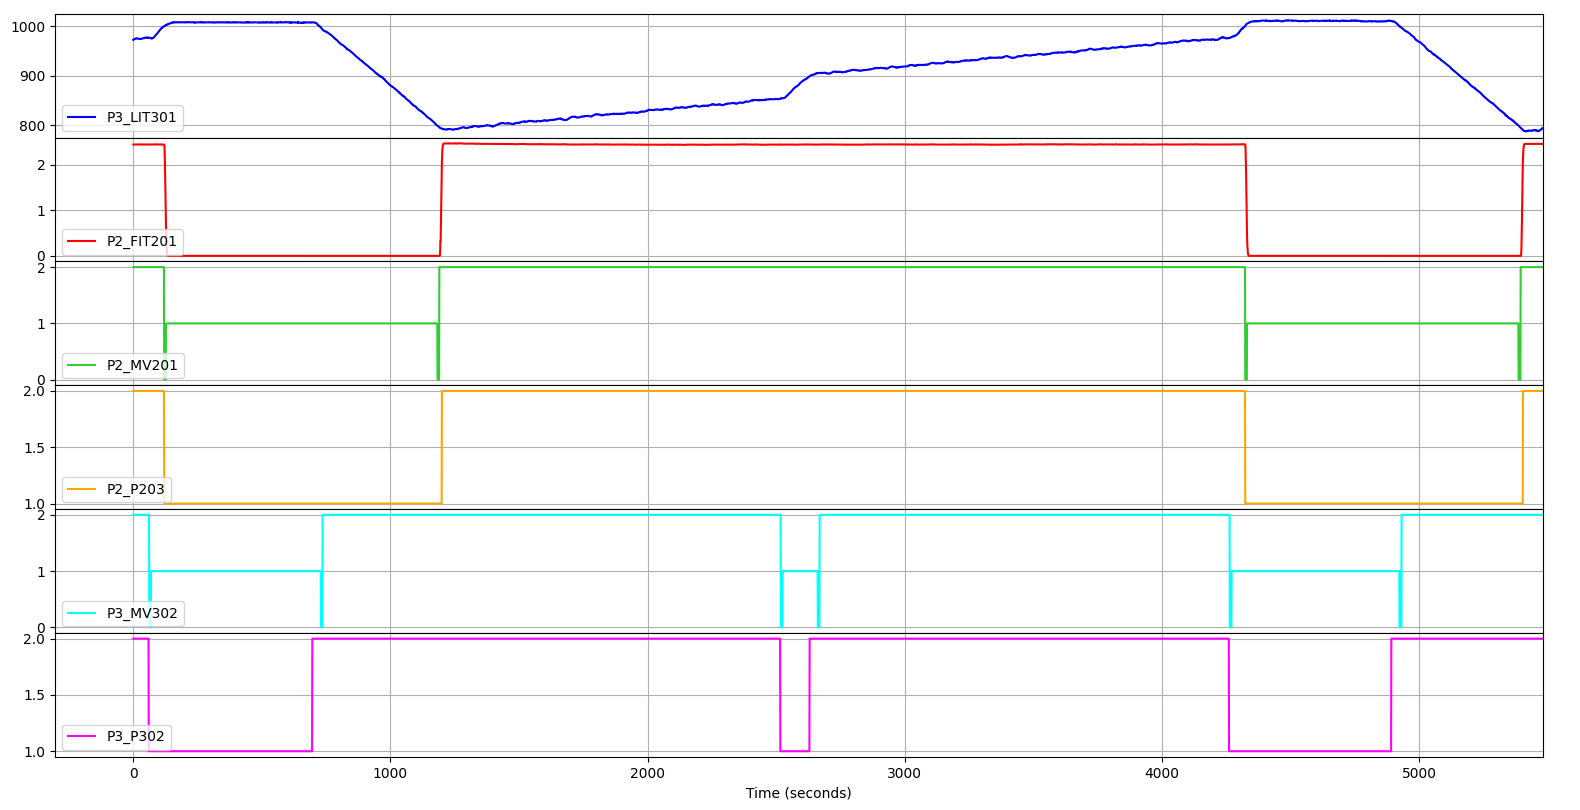
\includegraphics[scale=0.35]{chap6/P2P3_7.png}
	\caption{Verifying the conjecture about valve \texttt{P2\_MV201} }
	\label{fig:6_graphs_P2P3_mv201}
\end{figure}

\bigskip
Figure \ref{fig:6_graphs_P2P3_mv201} shows the particular behavior of \texttt{P3\_LIT103}, with two slope changes during the tank filling period. These slope changes correspond approximately to the relative setpoints found for \texttt{P3\_MV302} and \texttt{P3\_P302}. However, we will analyze this aspect later.
What we can see in relation to the initial conjecture about the role of \texttt{P2\_MV201} is that the period during which the valve remains in the ON state corresponds exactly to the increasing trend of \texttt{P3\_LIT301}. The conjecture thus finds further support. We also note how \texttt{P2\_FIT201} is related to the trend of \texttt{P2\_MV201} and the increasing trend of \texttt{P3\_LIT301}. 

\bigskip
Now let's examine the relationships between the tank represented by \texttt{P3\_LIT301} and the other actuators of PLC3 through Figure \ref{fig:6_graphs_P3}.

\begin{figure}[ht]
	\centering
	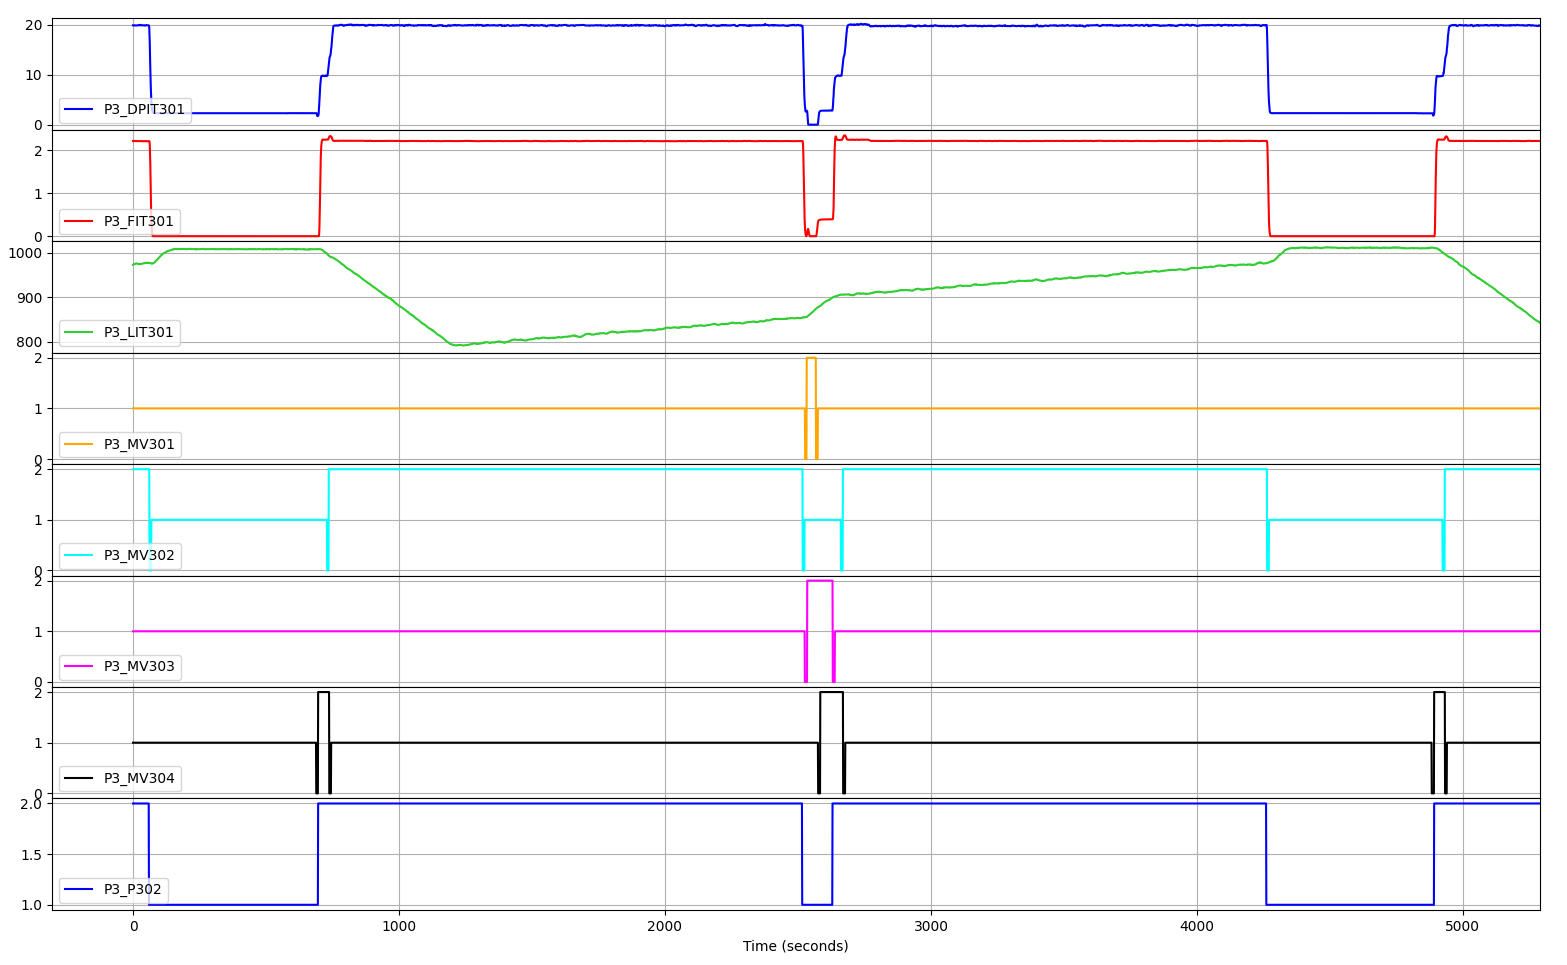
\includegraphics[scale=0.35]{chap6/P3_3.png}
	\caption{PLC3 registers}
	\label{fig:6_graphs_P3}
\end{figure}

From the charts, it is evident that the trends of \texttt{P3\_DPIT301} and \texttt{P3\_FIT301} exhibit similarities. Furthermore, their overall pattern closely follows that of the valve \texttt{P3\_MV302}. Based on these observations, we can speculate that there is a relationship between these registers or that they serve similar functions, possibly as p\textbf{ressure or flow sensors}.

\bigskip
Regarding pump \texttt{P3\_P302}, we observe that its OFF state coincides with the increasing slope of P3\_LIT301 during its upward trend and the entire phase when the level remains relatively stable. Conversely, its ON state corresponds to the gradual increase and decrease of the water level in the tank. This observation provides further evidence to support the hypothesis that \texttt{P3\_P302} is responsible for emptying the tank.

Valve \texttt{P3\_MV302} exhibits a similar pattern to pump \texttt{P3\_P302}. Building upon our previous findings, we can speculate that, similar to \texttt{P2\_MV201} in the previous analyzed subsystem, \texttt{P3\_MV302} is responsible for controlling the incoming flow to another element outside the analyzed subsystem.

\bigskip
Let us now analyze the potential roles of valves \texttt{P3\_MV301}, \texttt{P3\_MV303}, and \texttt{P3\_MV304} in relation to the indicated tank level. It seems unlikely that \texttt{P3\_MV304} has any direct impact on the tank level. The valve is activated twice within one system cycle, but there are no noticeable changes in \texttt{P3\_LIT301} during its first opening. This suggests that the second opening is also insignificant in terms of tank level. However, it is worth noting the slight peaks in \texttt{P3\_FIT301} that occur shortly after the valve's opening.

Regarding the remaining valves, \texttt{P3\_MV301} and \texttt{P3\_MV303}, their impact on the tank level is still unclear, particularly during the increased slope of \texttt{P3\_LIT101} around the second 2500. Figure \ref{fig:6_graphs_P3_zoom}  provides us with a comprehensive overview of the situation.

\vfill
\pagebreak
\begin{figure}[H]
	\centering
	\begin{subfigure}{0.90\textwidth}
		\includegraphics[width=\textwidth]{chap6/P3_8.png}
		\caption{}
		\label{subfig:6_mv301}
	\end{subfigure}
%\end{figure}
%\begin{figure}[H]\ContinuedFloat
	\begin{subfigure}{0.90\textwidth}
		\includegraphics[width=\textwidth]{chap6/P3_8b.png}
		\caption{}
		\label{subfig:6_mv301_zoom}
	\end{subfigure}
	\caption{\texttt{P3\_MV301} and \texttt{P3\_MV303} analysis}
	\label{fig:6_graphs_P3_zoom}
\end{figure}

The analysis of the valves \texttt{P3\_MV301} and \texttt{P3\_MV303} indeed presents some challenges. However, upon closer examination of Figure \ref{subfig:6_mv301_zoom}, we observe that when these valves are in the ON state, the slope of \texttt{P3\_LIT301} remains relatively constant. This is unexpected, as one would anticipate a steeper slope due to the inflow of liquid. Additionally, in Figure \ref{subfig:6_mv301}, we can observe that when these valves are in the OFF state, the slope of \texttt{P3\_LIT301} from the second 4300 remains similar to the section we are currently analyzing. Based on these observations, we speculate that these valves either \textbf{do not affect the water level of the tank} or have a minimal, undetectable impact.

\bigskip
Indeed, Figure \ref{fig:6_graphs_P3} provides additional insights into the relationship between the valves \texttt{P3\_MV301}, \texttt{P3\_MV303}, and \texttt{P3\_MV304} and the sensors \texttt{P3\_DPIT301} and \texttt{P3\_FIT301}. The graph shows that the values of \texttt{P3\_DPIT301} and \texttt{P3\_FIT301} undergo noticeable changes during the activation of these valves, suggesting a potential connection between them. This observation supports the hypothesis that the valves and sensors are linked in some way.

\subsubsection{Invariant Inference and Analysis}
\label{subsubsec:6_P2P3_invariants}

\paragraph{General Invariants}
\label{par:6_P2P3_general_invariant}

The analysis of general invariants does not yield any significant insights. However, it confirms the maximum and minimum values of the measurements seen in Section \ref{par:6_P2P3_measures_actuators_recognition} and identifies the presence of the spare actuator \texttt{P3\_P301}. 

\paragraph{Analysis on Single Actuator States}
\label{par:6_P2P3_single_act_states}
The analysis of single actuator states reveals additional information. The resulting invariants provide further support for the conjecture regarding the roles of \texttt{P2\_MV201} and \texttt{P3\_P302} in regulating the water level in the tank, with the former responsible for filling and the latter for emptying. Listing \ref{lst:6_preproc_P2P3_conditional_invariants} presents the specific invariants involved in this analysis.

\begin{lstlisting}[language=bash, numbers=left, caption=Conditional Invariants for \texttt{P2\_MV201} and \texttt{P3\_P302}, label=lst:6_preproc_P2P3_conditional_invariants]
	===========================
	P2_MV201 == 1.0 && P3_LIT301 < max_P3_LIT301 - 20 && P3_LIT301 > min_P3_LIT301 + 24 
	===========================
	P3_P301 == P3_MV303 == P3_MV301 == P2_P205 == P2_P203 == P2_MV201 == 1.0
	P3_P302 == 2.0
	slope_P3_LIT301 == -1.0
	P3_FIT301 > P2_MV201
	P3_DPIT301 > P3_FIT301 > P3_P302
	...
	===========================
	P2_MV201 == 2.0 && P3_LIT301 < max_P3_LIT301 - 20 && P3_LIT301 > min_P3_LIT301 + 24 
	===========================
	P2_P205 == P2_P203 == P2_MV201 == 2.0
	slope_P3_LIT301 == P2_P201
	P2_FIT201 > P2_MV201
	P2_FIT201 > P2_P201
	P2_FIT201 > P3_FIT301
	...
	===========================
	P3_P302 == 1.0 && P3_LIT301 < max_P3_LIT301 - 20 && P3_LIT301 > min_P3_LIT301 + 24 
	===========================
	P2_P205 == P2_P203 == P2_MV201 == 2.0
	slope_P3_LIT301 == P3_P302 == P2_P201
	P2_FIT201 > P2_MV201
	P2_FIT201 > P3_FIT301
	...
	===========================
	P3_P302 == 2.0 && P3_LIT301 < max_P3_LIT301 - 20 && P3_LIT301 > min_P3_LIT301 + 24 
	===========================
	P2_MV201 one of { 1.0, 2.0 }
	slope_P3_LIT301 one of { -1.0, 1.0 }
	P3_DPIT301 > P3_P302 > slope_P3_LIT301
	...
\end{lstlisting}

Moreover, from the analysis of the invariants it becomes apparent that when \texttt{P3\_P302} is in the ON state and \texttt{P2\_MV201} is in the OFF state, both \texttt{P3\_FIT301} and \texttt{P3\_DPIT301} take values greater than 2 (as derived from lines 5, 7, 8 and 32 of the listing). 

\bigskip
Regarding the valves \texttt{P3\_MV301} and \texttt{P3\_MV303}, Daikon's analysis does not provide specific information about their behavior during changes in slope when the water level rises. Therefore, further analysis is required to understand their role in the system.

However, one observation can be made regarding \texttt{P3\_MV304}. Daikon's analysis reveals two different slopes (increasing and decreasing) when this valve is in the ON state, which aligns with the observations made in the Graphical Analysis in Section \ref{subsubsec:6_P2P3_graphs}. This finding strengthens the conecture that \texttt{P3\_MV304} does not play a significant role in the tank cycle represented by \texttt{P3\_LIT301}.

\paragraph{Analysis of the Current System Configuration}
\label{par:6_P2P3_current_system_conf}
To simplify the analysis and facilitate the interpretation of outcomes, two separate groups of actuators were analyzed. The first group consists of \texttt{P2\_MV201} and \texttt{P3\_P302}, which are conjectured to regulate the level of the tank. The second group includes \texttt{P3\_MV301}, \texttt{P3\_MV303}, and \texttt{P3\_MV304}, for which it is speculated that they do not play a role in regulating the tank level. This grouping allows for a clearer examination of the states of the system and provides an opportunity to gain a better understanding of the behavior of these actuators. By analyzing these two groups separately, it becomes easier to draw conclusions and make comparisons between the different sets of actuators.

\bigskip
The analysis of the first group of actuators, specifically \texttt{P2\_MV201} and \texttt{P3\_P302}, further supports the conjectures made regarding their behavior in relation to the trend of the tank level. It was necessary to refine the analysis manually using the \texttt{runDaikon.py} script to obtain more detailed insights, particularly for the state \texttt{[P2\_MV201 == 2, P3\_P302 == 2]}. 

Regarding the second group of actuators, the analysis of their states only reinforces the hypothesis that their activation does not have a significant impact on the trend of tank level represented by \texttt{P3\_LIT301}. 

\bigskip
Unfortunately, no further useful information can be derived from this phase of the analysis. To address the remaining questions and clarify any outstanding issues, we will proceed to the next and final phase of the subsystem analysis.

\vfill

\subsubsection{Business Process Mining and Analysis}
\label{subsubsec:6_P2P3_bpa}

One of the hypotheses that needed to be tested was whether the valves \texttt{P3\_MV301}, \texttt{P3\_MV303}, and \texttt{P3\_MV304} have an impact on the tank level in the section between setpoints 850 and 900. Our initial assumption was that these actuators do not affect the level detected by \texttt{P3\_LIT301} because, as observed in the Graphical Analysis, the slope in that interval is similar to the slope between setpoints 970 and 1000, where these valves are not involved.

To verify this conjecture, we utilized the JSON file generated by the \texttt{processMining.py} script. This script allows us to isolate the specific intervals and calculate the slope for each of them. In Listing \ref{lst:6_preproc_P2P3_bp1}, we present the outcomes of these calculations, providing further insights into the behavior of the valves during those intervals.

\begin{lstlisting}[language=bash, numbers=left, caption=Slope calculation of \texttt{P3\_LIT301} for the 850-900 and 970-1000 intervals related to tank levels, label=lst:6_preproc_P2P3_bp1]
	"slope_P3_LIT301": [
	0.383, # from 970 to 1000
	0.395, # from 850 to 900
	0.384,
	0.395,
	0.354,
	0.38,
	0.388,
	0.381,
	0.385,
	0.386
	],
\end{lstlisting}

The provided data in Listing \ref{lst:6_preproc_P2P3_bp1} illustrates the calculated slopes for the intervals between 970 and 1000 (odd-numbered lines) and the intervals between 850 and 900 (even-numbered lines). Upon examination, we observe that the values for these two intervals are nearly identical, accounting for some expected fluctuations. This finding reinforces our initial conjecture that the \texttt{P3\_MV301}, \texttt{P3\_MV303} and \texttt{P3\_MV304} valves do not play a role in the process of filling and emptying the tank. It is indeed possible to speculate that the \texttt{P3\_MV30x} valves, similar to \texttt{P3\_MV302}, might have a role in a different part of the system that has not been analyzed in the current context. 

\bigskip
Based on the activity diagram obtained from the analysis of actuators \texttt{P2\_MV201} and \texttt{P3\_P302} (Figure \ref{fig:6_P2P3_process_mining}), the behavior of subsystem PLC2-3 can be summarized as follows:

\begin{itemize}
	\item When the system is in the states \texttt{[P2\_MV201 == 2, P3\_P302 == 2]} and \texttt{[P2\_MV201 == 2, P3\_P302 == 1]}, the level of the tank represented by \texttt{P3\_LIT301} is increasing. The tank level exhibits a faster growth rate in the latter state.
	
	\item When the system is in the state \texttt{[P2\_MV201 == 1, P3\_P302 == 1]}, the tank level remains stable.
	
	\item When the system is in the state \texttt{[P2\_MV201 == 1, P3\_P302 == 2]}, the tank level is decreasing.
\end{itemize}

The \textbf{absolute setpoints} for the tank level in subsystem PLC2-3 are defined as follows: the minimum setpoint is 800, the maximum setpoint is 1000, and there are additional setpoints at 850, 900, and 970, which correspond to specific changes in the slope of the tank level.

\bigskip
Taking a closer look at the behavior of sensors \texttt{P2\_FIT201} and \texttt{P3\_FIT301}, we observe the following patterns: \texttt{P2\_FIT201}, which is associated with incoming water flow and connected to valve \texttt{P2\_MV201}, exhibits values greater than 2 when the valve is in the ON state. Conversely, when the valve is set to OFF, the sensor reading drops to 0.

Regarding \texttt{P3\_FIT301}, it appears to be linked to the behavior of the pump \texttt{P3\_P301} and correlates with the water flow out of the tank. When the pump is activated and in the ON state, the sensor records values greater than 2. On the other hand, when the pump is turned off and in the OFF state, the sensor reading returns to 0.

\pagebreak
%\begin{comment}
\begin{figure}[H]
	\centering
	\includegraphics[scale=0.48]{chap6/business_process_P2P3a.png}
	\caption{Activity diagram for PLC2-3}
	\label{fig:6_P2P3_process_mining}
\end{figure}
%\end{comment}
\pagebreak

\vfill

\subsubsection{Properties}
\label{subsubsec:6_P2P3_summary_table}
Table \ref{table:6_P2P3_summarize_properties} provides a summary of the properties inferred from the conjectures made throughout the different stages of the analysis.

\bigskip
{\footnotesize
	\begin{longtable}[l]{p{0.05\textwidth} p{0.57\textwidth} p{0.30\textwidth}}
		\hline
		\textbf{\#} & \textbf{Statement} & \textbf{Derived from} \\
		\hline
		
		P23 & The registers \texttt{P3\_DPIT301}, \texttt{P3\_FIT301}, and \texttt{P3\_LIT301} of PLC3 hold likely sensor measurements. & Preliminary Analysis\newline Graphical Analysis \\
		\hline
		
		P24 & The registers \texttt{P3\_MV301}, \texttt{P3\_MV302}, \texttt{P3\_MV303}, \texttt{P3\_MV304}, and \texttt{P3\_P302} of PLC3 hold likely actuator commands. & Preliminary Analysis\newline Graphical Analysis \\
		\hline
		
		P25 & The register \texttt{P3\_P301} of PLC3 is associated to a spare actuator. & Preliminary Analysis\newline Graphical Analysis\newline Invariant Analysis \\
		\hline
		
		P26 & The register \texttt{P3\_LIT301} of PLC3 is associated to the level sensor of the tank controlled by PLC3. & Preliminary Analysis\newline Graphical Analysis \\
		\hline
		
		P27 & \texttt{P2\_MV201} and \texttt{P3\_P302} are are associated to the actuators responsible for the level behavior of the water contained in the tank. & Graphical Analysis\newline Invariant Analysis\newline Business Process \\
		\hline
		
		P28 & The rate of tank level growth is slow when both \texttt{P2\_MV201} and \texttt{P3\_P302} are in the ON state. The growth speed increases when \texttt{P3\_P302} switches to the OFF state. & Graphical Analysis\newline Business Process \\
		\hline
		
		P29 & When both \texttt{P2\_MV201} and \texttt{P3\_P302} are in the ON state, the inflow of water into the tank surpasses the outflow of water from the tank. & Graphical Analysis\newline Business Process \\
		\hline
		
		P30 & The tank level decreases when \texttt{P2\_MV201} is in the OFF state and \texttt{P3\_P302} is in the ON state. & Graphical Analysis\newline Invariant Analysis \\
		\hline
		
		P31 & The tank level remains (relatively) stable when both \texttt{P2\_MV201} and \texttt{P3\_P302} are in the OFF state. & Graphical Analysis\newline Business Process \\
		\hline
		
		P32 & The trend of the tank level switches from ascending to stable when the level reaches approximately 1000. It shifts from stable to descending when the level averages around 1012. It changes from descending back to ascending when the level reaches about 800. The slope of thank filling increases noticeably from around 850 to 900 and from around 970 to 1000. & Business Process \\
		\hline
		
		P33 & Absolute setpoints are 800, 850, 900, 970, 1000. & Business Process \\
		\hline
		
		P34 & \texttt{P2\_FIT201} is associated to a flow or pressure sensor to the \texttt{P3\_LIT301} register. It is related to the \texttt{P2\_MV201} valve. & Graphical Analysis\newline Invariant Analysis\newline Business Process\\
		\hline
		
		P35 & \texttt{P3\_FIT301} and \texttt{P3\_DPIT301} exhibit similar patterns in their behavior. Both registers are related to the operation of pump \texttt{P3\_P302} and, consequently, to the flow of water out of the tank. & Graphical Analysis\newline Business Process \\
		\hline
		
		P36 & The registers \texttt{P3\_MV301}, \texttt{P3\_MV303}, and \texttt{P3\_MV304} do not have an impact on the water level dynamics of the tank controlled by PLC3. & Graphical Analysis\newline Business Process \\
		\hline
		
		\caption{Properties of the PLC2-3 subsystem}
		\label{table:6_P2P3_summarize_properties}
	\end{longtable}
}

\subsection{Reverse Engineering of PLC3 and PLC4}
\label{subsec:6_P3P4_analysis}
In the final phase of the reverse engineering process, the focus is directed towards the subsystem consisting of PLC3 and PLC4 in the iTrust SWaT system. Given the constraints of the thesis, this section will provide a concise and schematic overview compared to the earlier sections.

\subsubsection{Pre-processing - Preliminary Analysis}
\label{subsubsec:6_P3P4_preprocessing}

\paragraph{Measurements and Actuators Recognition}
\label{par:6_P3P4_measures_actuators_recognition}

Listing \ref{lst:6_preproc_P3P4} shows the outcomes obtained from automatic recognition of likely measurements and actuators for PLC4. We omit those related to PLC3 as they are already known.

\begin{lstlisting}[language=bash, numbers=left, caption=Preliminary analysis outcomes for sensors and actuators of \texttt{PLC3-4}, label=lst:6_preproc_P3P4]
	Actuators: 
	...
	
	Sensors: 
	...
	P4_AIT401 {'max_lvl': 148.8, 'min_lvl': 148.8}
	P4_AIT402 {'max_lvl': 191.1, 'min_lvl': 185.5}
	P4_FIT401 {'max_lvl': 1.7, 'min_lvl': 1.7}
	P4_LIT401 {'max_lvl': 1002.8, 'min_lvl': 775.8}
	
	Hardcoded setpoints or spare actuators: 
	...
	P4_P401 [1.0]
	P4_P402 [2.0]
	P4_P403 [1.0]
	P4_P404 [1.0]
	P4_UV401 [2.0]
\end{lstlisting}

From the information provided in Listing \ref{lst:6_preproc_P3P4}, several observations can be made. Firstly, it is noted that there are no apparent actuators listed in the analysis. The likely sensors identified include \texttt{P4\_AIT401}, \texttt{P4\_AIT402}, \texttt{P4\_FIT401}, and \texttt{P4\_LIT401}. Among these sensors, \texttt{P4\_LIT401} is presumed to be the level sensor for the tank controlled by PLC4 based on similarities with the previous cases.

\bigskip
It is acknowledged that \texttt{P4\_FIT401} and \texttt{P4\_AIT401} are recognized as sensors, despite their seemingly constant values. It is important to note that the script used to identify likely actuators and sensors rounds the values to the first decimal place. Therefore, it is inferred that these registers contain continuous data with narrow value ranges.

Drawing on the analogy with the P21 property mentioned in Section \ref{subsubsec:6_P1P2_summary_table}, it is speculated that the \texttt{P4\_AIT40x} registers represent measurements related to some water property. Additionally, \texttt{P4\_FIT401} is speculated to represent a pressure or flow sensor, based on similarities observed in previous cases.

\bigskip
In the analysis of the hardcoded setpoints and spare actuators, two registers stand out: \texttt{P4\_P402} and \texttt{P4\_UV401}, both with a value of 2. Drawing on analogies from previous cases, \texttt{P4\_P402} is speculated to represent a pump that is constantly in the ON state and therefore active. However, regarding \texttt{P4\_UV401}, it is unclear whether it is an actuator, a hardcoded setpoint, or a different type of register. Further analysis is needed to determine its exact purpose and functionality within the system.

On the other hand, it can be concluded that \texttt{P4\_P401}, \texttt{P4\_P403}, and \texttt{P4\_P404} are spare actuators, specifically pumps. 

\paragraph{Actuator State Durations}
\label{par:6_P3P4_actuators_duration}
Since there are no state-changing actuators within PLC4, further analysis regarding the duration of actuator states will not be performed for this subsystem. Please refer to Section \ref{par:6_P2P3_actuators_duration} for evaluations of the duration of actuator states in PLC3.

\paragraph{Actuator State Changes}
\label{par:6_preproc_P3P4_actuator_state_changes}
As previously mentioned, our assumption is that P4\_LIT401 serves as the level sensor for the tank controlled by PLC4. In our analysis of PLC2-3, we speculated that \texttt{P3\_MV302} acted as a valve responsible for the incoming flow to an external element outside of that subsystem. To test this hypothesis, we examine the setpoints of \texttt{P3\_MV302} in relation to the level of tank \texttt{P4\_LIT401}. The setpoints of \texttt{P3\_MV302} corresponding to the tank level are presented in Listing \ref{lst:6_P3P4_preproc_changestate}.

\begin{lstlisting}[language=bash, numbers=left, caption=\texttt{P3\_MV302} state changes in relation to \texttt{P4\_LIT401}, label=lst:6_P3P4_preproc_changestate]
	Actuator state changes:
	...
	P3_MV302  prev_P3_MV302  P4_LIT401
	       0              2  1000.5510
	       0              1   784.4911
	       0              2   922.1866
	       0              1   881.0818
	       0              2  1000.2820
	       0              1   786.1061
	       0              2   922.8018
	       0              1   881.8508
	     ...            ...        ...
\end{lstlisting}

The initial analysis suggests a potential correlation between the tank level values of \texttt{P4\_LIT401} and the behavior of \texttt{P3\_MV302}. The ON state of \texttt{P3\_MV302} aligns with an increase in the tank level, while the OFF state corresponds to a decrease. However, further analysis is required to provide additional evidence and support for this conjecture.
\vfill

\subsubsection{Graphs and Statistical Analysis}
\label{subsubsec:6_P3P4_graphs}
We will attempt to gain a deeper understanding of the pattern exhibited by the PLC4 registers by referencing Figure \ref{fig:6_graph_P4}.

\begin{figure}[ht]
	\centering
	\includegraphics[scale=0.35]{chap6/P4_1.png}
	\caption{PLC4 registers}
	\label{fig:6_graph_P4}
\end{figure}

The image reveals interesting behavior in the \texttt{P4\_AIT401} and \texttt{P4\_AIT401} registers. Notably, \texttt{P4\_AIT401} exhibits a linear trend rather than a cyclic one, with values oscillating within a narrow range. This suggests that, similar to \texttt{P2\_AIT201} (refer to Section \ref{subsubsec:6_P2P3_graphs}), this register may correspond to a sensor measuring a specific water property. On the other hand, \texttt{P4\_AIT402} appears to follow the level trend of sensor \texttt{P4\_LIT401}, but with a downward cyclic pattern where each cycle starts at a lower level than the previous one. Given the limited value range and the similarity in naming conventions, it is highly likely that this register represents another water property sensor rather than a tank.

Additionally, \texttt{P4\_FIT401} does not display a cyclic pattern like the other registers of the same type, and its values exhibit minimal variation, corroborating the findings from the previous analysis phase.

\bigskip
Now, let us refer to Figure \ref{fig:6_graph_P3P4_mv302} to seek confirmation regarding the conjecture that implicates valve \texttt{P3\_MV302} as the responsible actuator for tank filling.

\begin{figure}[ht]
	\centering
	\includegraphics[scale=0.35]{chap6/P3P4_mv302.png}
	\caption{\texttt{P3\_MV302} and \texttt{P4\_LIT401} behaviors}
	\label{fig:6_graph_P3P4_mv302}
\end{figure}

The image provides clear evidence that the behaviors of valve \texttt{P3\_MV302} and tank level sensor \texttt{P4\_LIT401} perfectly align. Additionally, \texttt{P3\_FIT301} (and its corresponding sensor, \texttt{P3\_DPIT301}) appear to be related to the pattern observed in \texttt{P4\_LIT401}.
 
\bigskip
Upon closer observation, it becomes apparent that the tank controlled by PLC4 \textbf{does \textit{not} have plateau periods}. When the incoming water flow ceases, the tank immediately begins to empty. Based on our findings in previous subsystems, we speculate that the actuator responsible for tank emptying could be the pump indicated by register \texttt{P4\_P402}. This speculation is further supported by the nearly constant trend observed in sensor \texttt{P4\_FIT401}.

\bigskip
Figure \ref{fig:6_graph_P3P4_tanks} depicts the correlation between the tanks within this subsystem and the actuators that are responsible for their filling cycle.

\begin{figure}[ht]
	\centering
	\includegraphics[scale=0.35]{chap6/P3P4_tanks.png}
	\caption{Tanks in subsystem PLC3-4 and their correlation.}
	\label{fig:6_graph_P3P4_tanks}
\end{figure}

\bigskip
Further analysis was conducted to investigate whether valves \texttt{P3\_MV301}, \texttt{P3\_MV303}, and \texttt{P3\_MV304} played a role in the tank filling cycle of PLC4. However, the analysis did not confirm this hypothesis. Therefore, it can be speculated that these valves are connected to other parts of the system that are not currently discussed in this analysis.

\subsubsection{Invariant Inference and Analysis}
\label{subsubsec:6_P3P4_invariants}
The invariant analysis for the subsystem consisting of PLC3-4 will be brief as the states of the subsystem align with the states of valve \texttt{P3\_MV302}, with \texttt{P4\_P402} being constant throughout.

\paragraph{General Invariants}
\label{par:6_P3P4_general_invariant}
Again, the analysis of the general invariants offers no new information compared to what we conjectured earlier. We therefore continue with the analysis of the current system configuration.

\paragraph{Analysis of the Current System Configuration}
\label{par:6_P3P4_current_system_conf}
The analysis of the current system configuration provides confirmation that when the system is in the state \texttt{[P3\_MV302 == 1, P4\_P402 == 2]}, the tank level, as indicated by sensor \texttt{P4\_LIT401}, shows a decreasing slope. Additionally, it is noted that the spare actuators align with the expected behavior. 

However, in the state \texttt{[P3\_MV302 == 2, P4\_P402 == 2]}, the invariants generated by Daikon do not provide the anticipated slope data, which was expected to be increasing based on previous observations. This is due to the descending slope between levels 880 and 925 of the tank represented by \texttt{P4\_LIT401}: by refining the analysis between the two increasing slope sections we get the correct outcome, as shown in Listing \ref{lst:6_preproc_P3P4_refine_analysis}.

\begin{lstlisting}[language=bash, numbers=left, caption=Daikon manual analysis for \texttt{P3\_MV302 == 2}, label=lst:6_preproc_P3P4_refine_analysis]
	===========================
	P3_MV302 == 2 && P4_P402 == 2 && P4_LIT401 < 990 && P4_LIT401 > 930
	===========================
	...
	slope_P4_LIT401 == slope_P3_LIT301 == P4_P404 == P4_P403 == P4_P401 == P3_P301 == P3_MV304 == P3_MV303 == P3_MV301 == 1.0
	...
\end{lstlisting}

\subsubsection{Business Process Mining and Analysis}
\label{subsubsec:6_P3P4_bpa}

The process mining step for the PLC3-4 subsystem is straightforward. In this phase, we will not focus on determining the chronological order of states (as we already know they correspond to the states of valve \texttt{P3\_MV302}). Instead, we will examine the setpoints and extract any available information concerning additional measurements.
Figure \ref{fig:6_P3P4_process_mining} presents the activity diagram depicting the subsystem under analysis.

\begin{figure}[ht]
	\centering
	\includegraphics[scale=0.60]{chap6/business_process_P3P4.png}
	\caption{Activity diagram for PLC3-4}
	\label{fig:6_P3P4_process_mining}
\end{figure}

\bigskip
The diagram provides confirmation that when the system is in the state \texttt{[P3\_MV302 == 2, P4\_P402 == 2]}, the tank level trend is increasing. Conversely, when the system is in the state \texttt{[P3\_MV302 == 2, P4\_P402 == 2]}, the trend is decreasing.

\bigskip
Regarding the setpoints, based on the standard deviation of the data from \texttt{P4\_LIT401}, the absolute setpoints for the system are as follows: 785 (minimum), 880 (relative minimum), 925 (relative maximum), and 1000 (maximum).

\bigskip
Furthermore, from the process mining phase, we can extract information about \texttt{P3\_FIT301} and \texttt{P3\_DPIT301}. \texttt{P3\_FIT301} registers values greater than 2 when both pump \texttt{P4\_P402} and valve \texttt{P3\_MV302} are in the ON state, while it drops to an average of 0.7 when the valve is off. Similarly, P3\_DPIT301 registers values close to 20 when the valve is ON, and these values decrease when the valve is OFF.
\vfill

\subsubsection{Properties}
\label{subsubsec:6_P3P4_summary_table}

Table \ref{table:6_P3P4_summarize_properties} provides a summary of the properties inferred from the conjectures made throughout the different stages of the analysis. Regrettably, we encountered difficulties in determining the type and purpose of the register labeled as \texttt{P4\_UV401}.

\bigskip
{\footnotesize
	\begin{longtable}[l]{p{0.05\textwidth} p{0.57\textwidth} p{0.30\textwidth}}
		\hline
		\textbf{\#} & \textbf{Statement} & \textbf{Derived from} \\
		\hline
		
		P37 & The registers \texttt{P4\_AIT401}, \texttt{P4\_AIT402}, \texttt{P4\_FIT401}, and \texttt{P4\_LIT401} of PLC4 hold likely sensor measurements. & Preliminary Analysis\newline Graphical Analysis \\
		\hline
		
		P38 & The register \texttt{P4\_P402} of PLC4 holds likely actuator command. Its status is constantly ON. & Preliminary Analysis\newline Graphical Analysis\newline Business Process \\
		\hline
		
		P39 & The registers \texttt{P4\_P401}, \texttt{P4\_P403}, and \texttt{P4\_P404} of PLC4 are associated to spare actuators. & Preliminary Analysis\newline Graphical Analysis\newline Invariant Analysis \\
		\hline
		
		P40 & The register \texttt{P4\_LIT401} of PLC4 is associated to the level sensor of the tank controlled by PLC4. & Preliminary Analysis\newline Graphical Analysis \\
		\hline
		
		P41 & \texttt{P3\_MV302} and \texttt{P4\_P402} are the actuators responsible for the level behavour of the water contanined in the tank controlled by PLC4. & Graphical Analysis\newline Invariant Analysis\newline Business Process \\
		\hline
		
		P42 & The level of the tank identified by the register \texttt{P4\_LIT401} increases when both \texttt{P3\_MV302} and \texttt{P4\_P402} are in the ON state. It decreases when \texttt{P3\_MV302} is in the OFF state. & Graphical Analysis\newline Invariant Analysis\newline Business Process \\
		\hline
		
		P43 & The trend of the tank level controlled by PLC4 transition from ascending to descending when the level reaches approximately 925 and 1000. It changes from descending when the level reaches approximately 785 and 880. & Business Process \\
		\hline
		
		P44 & Absolute setpoints are 785, 880, 925 and 1000 & Business Process \\
		\hline
		
		P45 & \texttt{P4\_FIT401} serves as a flow or pressure sensor to the \texttt{P4\_LIT401} register. It is related to the \texttt{P4\_P402} pump. & Graphical Analysis\newline Business Process \\
		\hline
		
		P46 & \texttt{P4\_P401} does not exhibit a cyclic trend. & Graphical Analysis \\
		\hline
		
		P47 & The register \texttt{P4\_P402} exhibits a cyclic decreasing trend, which is closely linked to the trend observed in the \texttt{P4\_LIT401} register. & Graphical Analysis\\
		\hline
		
		P48 & Both \texttt{P4\_AIT401} and \texttt{P4\_AIT402} serves as sensors for measuring certain properties of the water. & Preliminary Analysis\newline Graphical Analysis \\
		\hline
		
		P49 & The registers \texttt{P3\_MV301}, \texttt{P3\_MV303}, and \texttt{P3\_MV304} do not have an impact on the water level dynamics on the tank controlled by PLC4. & Graphical Analysis\newline Business Process \\
		\hline
		
		\caption{Properties of the PLC3-4 subsystem}
		\label{table:6_P3P4_summarize_properties}
	\end{longtable}
}

\section{PLCs Architecture}
In Table \ref{table:6_plc_registers_summary}, we present an overview of the architecture of the four analyzed PLCs derived from the previous phases of the analysis. For each PLC, we provide details about its constituent registers, including their operational range. Where possible, we also indicate the role of these registers within the physical system. By combining the information presented in Tables \ref{table:6_P1P2_summarize_properties}, \ref{table:6_P2P3_summarize_properties}, and \ref{table:6_P3P4_summarize_properties} with the content of Table \ref{table:6_plc_registers_summary}, we can consider the reverse engineering process implemented in this analysis to be complete. 
To enhance readability, we will assign integer numbers to tanks based on the PLCs that control them. For example, Tank 1 represents the tank associated with PLC1, Tank 3 represents the tank associated with PLC3, and so forth.

\bigskip
{\small
	\begin{longtable}[c]{p{0.10\textwidth} p{0.50\textwidth} p{0.13\textwidth} p{0.18\textwidth}}
		\hline
		\textbf{PLC} & \textbf{Physical device / Variable} & \textbf{Range} & \textbf{PLC register} \\ [0.5ex] 
		\hline
		\multirow{5}{12em}{PLC1} & Level sensor for Tank 1 & [489-815] & \texttt{P1\_LIT101} \\ 
		& Flow or pressure sensor & [0-2.7] & \texttt{P1\_FIT101} \\
		& Valve for Tank 1 inflow water & \{0,1,2\} & \texttt{P1\_MV101} \\ 
		& Pump for Tank 1 outflow water & \{0,1\} & \texttt{P1\_P101} \\
		& Spare actuator (OFF) & 1 & \texttt{P1\_P102} \\
		\hline
		\multirow{11}{12em}{PLC2} & Flow or pressure sensor & [0-2.4] & \texttt{P2\_FIT201} \\
		& Sensor for some water property & [252-256] & \texttt{P2\_AIT201} \\
		& Sensor for some water property & [8.3-8.4] & \texttt{P2\_AIT202} \\
		& Unkown & [320-342] & \texttt{P2\_AIT203} \\
		& Valve for Tank 3 inflow water & \{0,1,2\} & \texttt{P2\_MV201} \\
		& Spare actuator (OFF) & 1 & \texttt{P2\_P201} \\
		& Spare actuator (OFF) & 1 & \texttt{P2\_P202} \\
		& Pump (unknown role) & \{0.1\} & \texttt{P2\_P203} \\
		& Spare actuator (OFF) & 1 & \texttt{P2\_P204} \\
		& Pump (unknown role) & \{0.1\} & \texttt{P2\_P205} \\
		& Spare actuator (OFF) & 1 & \texttt{P2\_P206} \\
		\hline
		\multirow{9}{12em}{PLC3} & Level sensor for Tank 3 & [768-1014] & \texttt{P3\_LIT301} \\
		& Flow or pressure sensor & [0-2.4] & \texttt{P3\_FIT301} \\
		& Flow or pressure sensor & [0-20.4] & \texttt{P3\_DPIT301} \\
		& Valve (unkonw role) & \{0,1,2\} & \texttt{P3\_MV301} \\
		& Valve for Tank 4 inflow water & \{0,1,2\} & \texttt{P3\_MV302} \\
		& Valve (unkonw role) & \{0,1,2\} & \texttt{P3\_MV303} \\
		& Valve (unkonw role) & \{0,1,2\} & \texttt{P3\_MV304} \\
		& Spare actuator (OFF) & 1 & \texttt{P3\_P301} \\
		& Pump for Tank 3 outflow water & [0,1] & \texttt{P3\_P302} \\
		\hline
		\multirow{9}{12em}{PLC4} & Level sensor for Tank 4 & [775-1002] & \texttt{P4\_LIT401} \\
		& Flow or pressure sensor & [1.7] & \texttt{P4\_FIT401} \\
		& Sensor for some water property & [148.8] & \texttt{P4\_AIT401} \\
		& Sensor for some water property & [185-191] & \texttt{P4\_AIT402} \\
		& Spare actuator & 1 & \texttt{P4\_P401} \\
		& Pump for Tank 4 outflow water & 2 & \texttt{P4\_P402} \\
		& Spare actuator & 1 & \texttt{P4\_P403} \\
		& Spare actuator & 1 & \texttt{P4\_P404} \\
		& Unknown & 2 & \texttt{P4\_UV401} \\
		\hline
		
		\caption{Summary of the reconstructed composition PLCs from 1 to 4 in the iTrust SWaT System}
		\label{table:6_plc_registers_summary}
	\end{longtable}
}
\vfill
\nolinenumbers

%###### CAPITOLO 7 ######%
\chapter{Conclusions}
\label{conclusions}

\section{Discussions}
\label{sec:discussion}

\section{Guidelines}
\label{sec:guidelines}

\section{Future work}
\label{sec:futurework}

%##### LISTA FIGURE #####%
\cleardoublepage
\addcontentsline{toc}{chapter}{\listfigurename}
\listoffigures

%##### LISTA TABELLE #####%
\cleardoublepage
\addcontentsline{toc}{chapter}{\listtablename}
\listoftables

%###### BIBLIOGRAFIA ######%
\printbibliography[heading=bibintoc, title=References]

%%%%%%%%%%%%%%%%%%%%%%%%%%%%%%%%%
%		Fine TESI				%
%%%%%%%%%%%%%%%%%%%%%%%%%%%%%%%%%
\end{document}